% Options for packages loaded elsewhere
\PassOptionsToPackage{unicode}{hyperref}
\PassOptionsToPackage{hyphens}{url}
%
\documentclass[
  ignorenonframetext,
  aspectratio=169]{beamer}
\usepackage{pgfpages}
\setbeamertemplate{caption}[numbered]
\setbeamertemplate{caption label separator}{: }
\setbeamercolor{caption name}{fg=normal text.fg}
\beamertemplatenavigationsymbolsempty
% Prevent slide breaks in the middle of a paragraph
\widowpenalties 1 10000
\raggedbottom
\setbeamertemplate{part page}{
  \centering
  \begin{beamercolorbox}[sep=16pt,center]{part title}
    \usebeamerfont{part title}\insertpart\par
  \end{beamercolorbox}
}
\setbeamertemplate{section page}{
  \centering
  \begin{beamercolorbox}[sep=12pt,center]{part title}
    \usebeamerfont{section title}\insertsection\par
  \end{beamercolorbox}
}
\setbeamertemplate{subsection page}{
  \centering
  \begin{beamercolorbox}[sep=8pt,center]{part title}
    \usebeamerfont{subsection title}\insertsubsection\par
  \end{beamercolorbox}
}
\AtBeginPart{
  \frame{\partpage}
}
\AtBeginSection{
  \ifbibliography
  \else
    \frame{\sectionpage}
  \fi
}
\AtBeginSubsection{
  \frame{\subsectionpage}
}
\usepackage{amsmath,amssymb}
\usepackage{lmodern}
\usepackage{iftex}
\ifPDFTeX
  \usepackage[T1]{fontenc}
  \usepackage[utf8]{inputenc}
  \usepackage{textcomp} % provide euro and other symbols
\else % if luatex or xetex
  \usepackage{unicode-math}
  \defaultfontfeatures{Scale=MatchLowercase}
  \defaultfontfeatures[\rmfamily]{Ligatures=TeX,Scale=1}
\fi
\usecolortheme{orchid}
% Use upquote if available, for straight quotes in verbatim environments
\IfFileExists{upquote.sty}{\usepackage{upquote}}{}
\IfFileExists{microtype.sty}{% use microtype if available
  \usepackage[]{microtype}
  \UseMicrotypeSet[protrusion]{basicmath} % disable protrusion for tt fonts
}{}
\makeatletter
\@ifundefined{KOMAClassName}{% if non-KOMA class
  \IfFileExists{parskip.sty}{%
    \usepackage{parskip}
  }{% else
    \setlength{\parindent}{0pt}
    \setlength{\parskip}{6pt plus 2pt minus 1pt}}
}{% if KOMA class
  \KOMAoptions{parskip=half}}
\makeatother
\usepackage{xcolor}
\IfFileExists{xurl.sty}{\usepackage{xurl}}{} % add URL line breaks if available
\IfFileExists{bookmark.sty}{\usepackage{bookmark}}{\usepackage{hyperref}}
\hypersetup{
  pdftitle={Unsupervised Learning (in biological data analysis)},
  hidelinks,
  pdfcreator={LaTeX via pandoc}}
\urlstyle{same} % disable monospaced font for URLs
\newif\ifbibliography
\usepackage{color}
\usepackage{fancyvrb}
\newcommand{\VerbBar}{|}
\newcommand{\VERB}{\Verb[commandchars=\\\{\}]}
\DefineVerbatimEnvironment{Highlighting}{Verbatim}{commandchars=\\\{\}}
% Add ',fontsize=\small' for more characters per line
\usepackage{framed}
\definecolor{shadecolor}{RGB}{248,248,248}
\newenvironment{Shaded}{\begin{snugshade}}{\end{snugshade}}
\newcommand{\AlertTok}[1]{\textcolor[rgb]{0.94,0.16,0.16}{#1}}
\newcommand{\AnnotationTok}[1]{\textcolor[rgb]{0.56,0.35,0.01}{\textbf{\textit{#1}}}}
\newcommand{\AttributeTok}[1]{\textcolor[rgb]{0.77,0.63,0.00}{#1}}
\newcommand{\BaseNTok}[1]{\textcolor[rgb]{0.00,0.00,0.81}{#1}}
\newcommand{\BuiltInTok}[1]{#1}
\newcommand{\CharTok}[1]{\textcolor[rgb]{0.31,0.60,0.02}{#1}}
\newcommand{\CommentTok}[1]{\textcolor[rgb]{0.56,0.35,0.01}{\textit{#1}}}
\newcommand{\CommentVarTok}[1]{\textcolor[rgb]{0.56,0.35,0.01}{\textbf{\textit{#1}}}}
\newcommand{\ConstantTok}[1]{\textcolor[rgb]{0.00,0.00,0.00}{#1}}
\newcommand{\ControlFlowTok}[1]{\textcolor[rgb]{0.13,0.29,0.53}{\textbf{#1}}}
\newcommand{\DataTypeTok}[1]{\textcolor[rgb]{0.13,0.29,0.53}{#1}}
\newcommand{\DecValTok}[1]{\textcolor[rgb]{0.00,0.00,0.81}{#1}}
\newcommand{\DocumentationTok}[1]{\textcolor[rgb]{0.56,0.35,0.01}{\textbf{\textit{#1}}}}
\newcommand{\ErrorTok}[1]{\textcolor[rgb]{0.64,0.00,0.00}{\textbf{#1}}}
\newcommand{\ExtensionTok}[1]{#1}
\newcommand{\FloatTok}[1]{\textcolor[rgb]{0.00,0.00,0.81}{#1}}
\newcommand{\FunctionTok}[1]{\textcolor[rgb]{0.00,0.00,0.00}{#1}}
\newcommand{\ImportTok}[1]{#1}
\newcommand{\InformationTok}[1]{\textcolor[rgb]{0.56,0.35,0.01}{\textbf{\textit{#1}}}}
\newcommand{\KeywordTok}[1]{\textcolor[rgb]{0.13,0.29,0.53}{\textbf{#1}}}
\newcommand{\NormalTok}[1]{#1}
\newcommand{\OperatorTok}[1]{\textcolor[rgb]{0.81,0.36,0.00}{\textbf{#1}}}
\newcommand{\OtherTok}[1]{\textcolor[rgb]{0.56,0.35,0.01}{#1}}
\newcommand{\PreprocessorTok}[1]{\textcolor[rgb]{0.56,0.35,0.01}{\textit{#1}}}
\newcommand{\RegionMarkerTok}[1]{#1}
\newcommand{\SpecialCharTok}[1]{\textcolor[rgb]{0.00,0.00,0.00}{#1}}
\newcommand{\SpecialStringTok}[1]{\textcolor[rgb]{0.31,0.60,0.02}{#1}}
\newcommand{\StringTok}[1]{\textcolor[rgb]{0.31,0.60,0.02}{#1}}
\newcommand{\VariableTok}[1]{\textcolor[rgb]{0.00,0.00,0.00}{#1}}
\newcommand{\VerbatimStringTok}[1]{\textcolor[rgb]{0.31,0.60,0.02}{#1}}
\newcommand{\WarningTok}[1]{\textcolor[rgb]{0.56,0.35,0.01}{\textbf{\textit{#1}}}}
\usepackage{graphicx}
\makeatletter
\def\maxwidth{\ifdim\Gin@nat@width>\linewidth\linewidth\else\Gin@nat@width\fi}
\def\maxheight{\ifdim\Gin@nat@height>\textheight\textheight\else\Gin@nat@height\fi}
\makeatother
% Scale images if necessary, so that they will not overflow the page
% margins by default, and it is still possible to overwrite the defaults
% using explicit options in \includegraphics[width, height, ...]{}
\setkeys{Gin}{width=\maxwidth,height=\maxheight,keepaspectratio}
% Set default figure placement to htbp
\makeatletter
\def\fps@figure{htbp}
\makeatother
\setlength{\emergencystretch}{3em} % prevent overfull lines
\providecommand{\tightlist}{%
  \setlength{\itemsep}{0pt}\setlength{\parskip}{0pt}}
\setcounter{secnumdepth}{-\maxdimen} % remove section numbering
\AtBeginSection[]{\begin{frame}\frametitle{Today's lecture}\tableofcontents[currentsection]\end{frame}}
\makeatletter
\def\ps@titlepage{%
  \setbeamertemplate{footline}{}
}
\addtobeamertemplate{title page}{\thispagestyle{titlepage}}{}
\makeatother
\include{toc}
\ifLuaTeX
  \usepackage{selnolig}  % disable illegal ligatures
\fi

\title{Unsupervised Learning (in biological data analysis)}
\author{Yongjin Park\\
University of British Columbia\\
(with contributions from Drs. Korthauer, Mostafavi)}
\date{25 February, 2022}

\begin{document}
\frame{\titlepage}

\begin{frame}[fragile]{Little update on the lecture format}
\protect\hypertarget{little-update-on-the-lecture-format}{}
\begin{itemize}
\item
  Minimized the lines of codes exposed \ldots{}
\item
  However, the \texttt{Rmd} file for this lecture is available in the
  github repo:
\end{itemize}

\begin{verbatim}
https://github.com/STAT540-UBC/lectures
\end{verbatim}

\begin{itemize}
\item
  You can check out \texttt{R} and \texttt{torch} codes to run them
  yourself.
\item
  ``I do not understand what I cannot create'' - Richard Feynman
\end{itemize}
\end{frame}

\hypertarget{general-discussions-on-unsupervised-learning}{%
\section{General discussions on unsupervised
learning}\label{general-discussions-on-unsupervised-learning}}

\begin{frame}{What is Unsupervised Learning?}
\protect\hypertarget{what-is-unsupervised-learning}{}
\begin{columns}[T]
\begin{column}{.45\textwidth}
\begin{block}{Supervised learning}
\protect\hypertarget{supervised-learning}{}
\begin{itemize}
\item
  Input: data \(\mathcal{X} = \{\mathbf{x}_{i},\ldots\}\)
\item
  Input 2: label \(\mathcal{Y} = \{y_{i},\ldots\}\)
\item
  Goal: learn \(f: \mathcal{X} \to \mathcal{Y}\)
\end{itemize}
\end{block}

X: gene expression samples; Y: disease labels
\end{column}

\begin{column}{.45\textwidth}
\begin{block}{Unsupervised learning}
\protect\hypertarget{unsupervised-learning}{}
\begin{itemize}
\item
  Input: data \(\mathcal{X} = \{\mathbf{x}_{i},\ldots\}\)
\item
  Goal 1: learn \(f: \mathcal{Z} \to \mathcal{X}\)
\item
  Goal 2: hidden/latent states,
  \(\mathcal{Z} = \{\mathbf{z}_{i},\ldots\}\)
\end{itemize}
\end{block}

X: gene expression matrices
\end{column}
\end{columns}
\end{frame}

\begin{frame}{The goal of unsupervised learning: Find a good
representation of high-dimensional data}
\protect\hypertarget{the-goal-of-unsupervised-learning-find-a-good-representation-of-high-dimensional-data}{}
What is a \textbf{good representation} of high-dimensional biology data
\textbf{to our purpose}?

\begin{enumerate}
\item
  What are the properties of high-dimensional data?

  \begin{itemize}
  \tightlist
  \item
    Continuous vs.~discrete? Count vs.~intensity?
  \end{itemize}
\item
  What do we mean by a ``good'' representation?
\item
  What is our purpose of unsupervised learning?
\end{enumerate}
\end{frame}

\begin{frame}{Why unsupervised learning?}
\protect\hypertarget{why-unsupervised-learning}{}
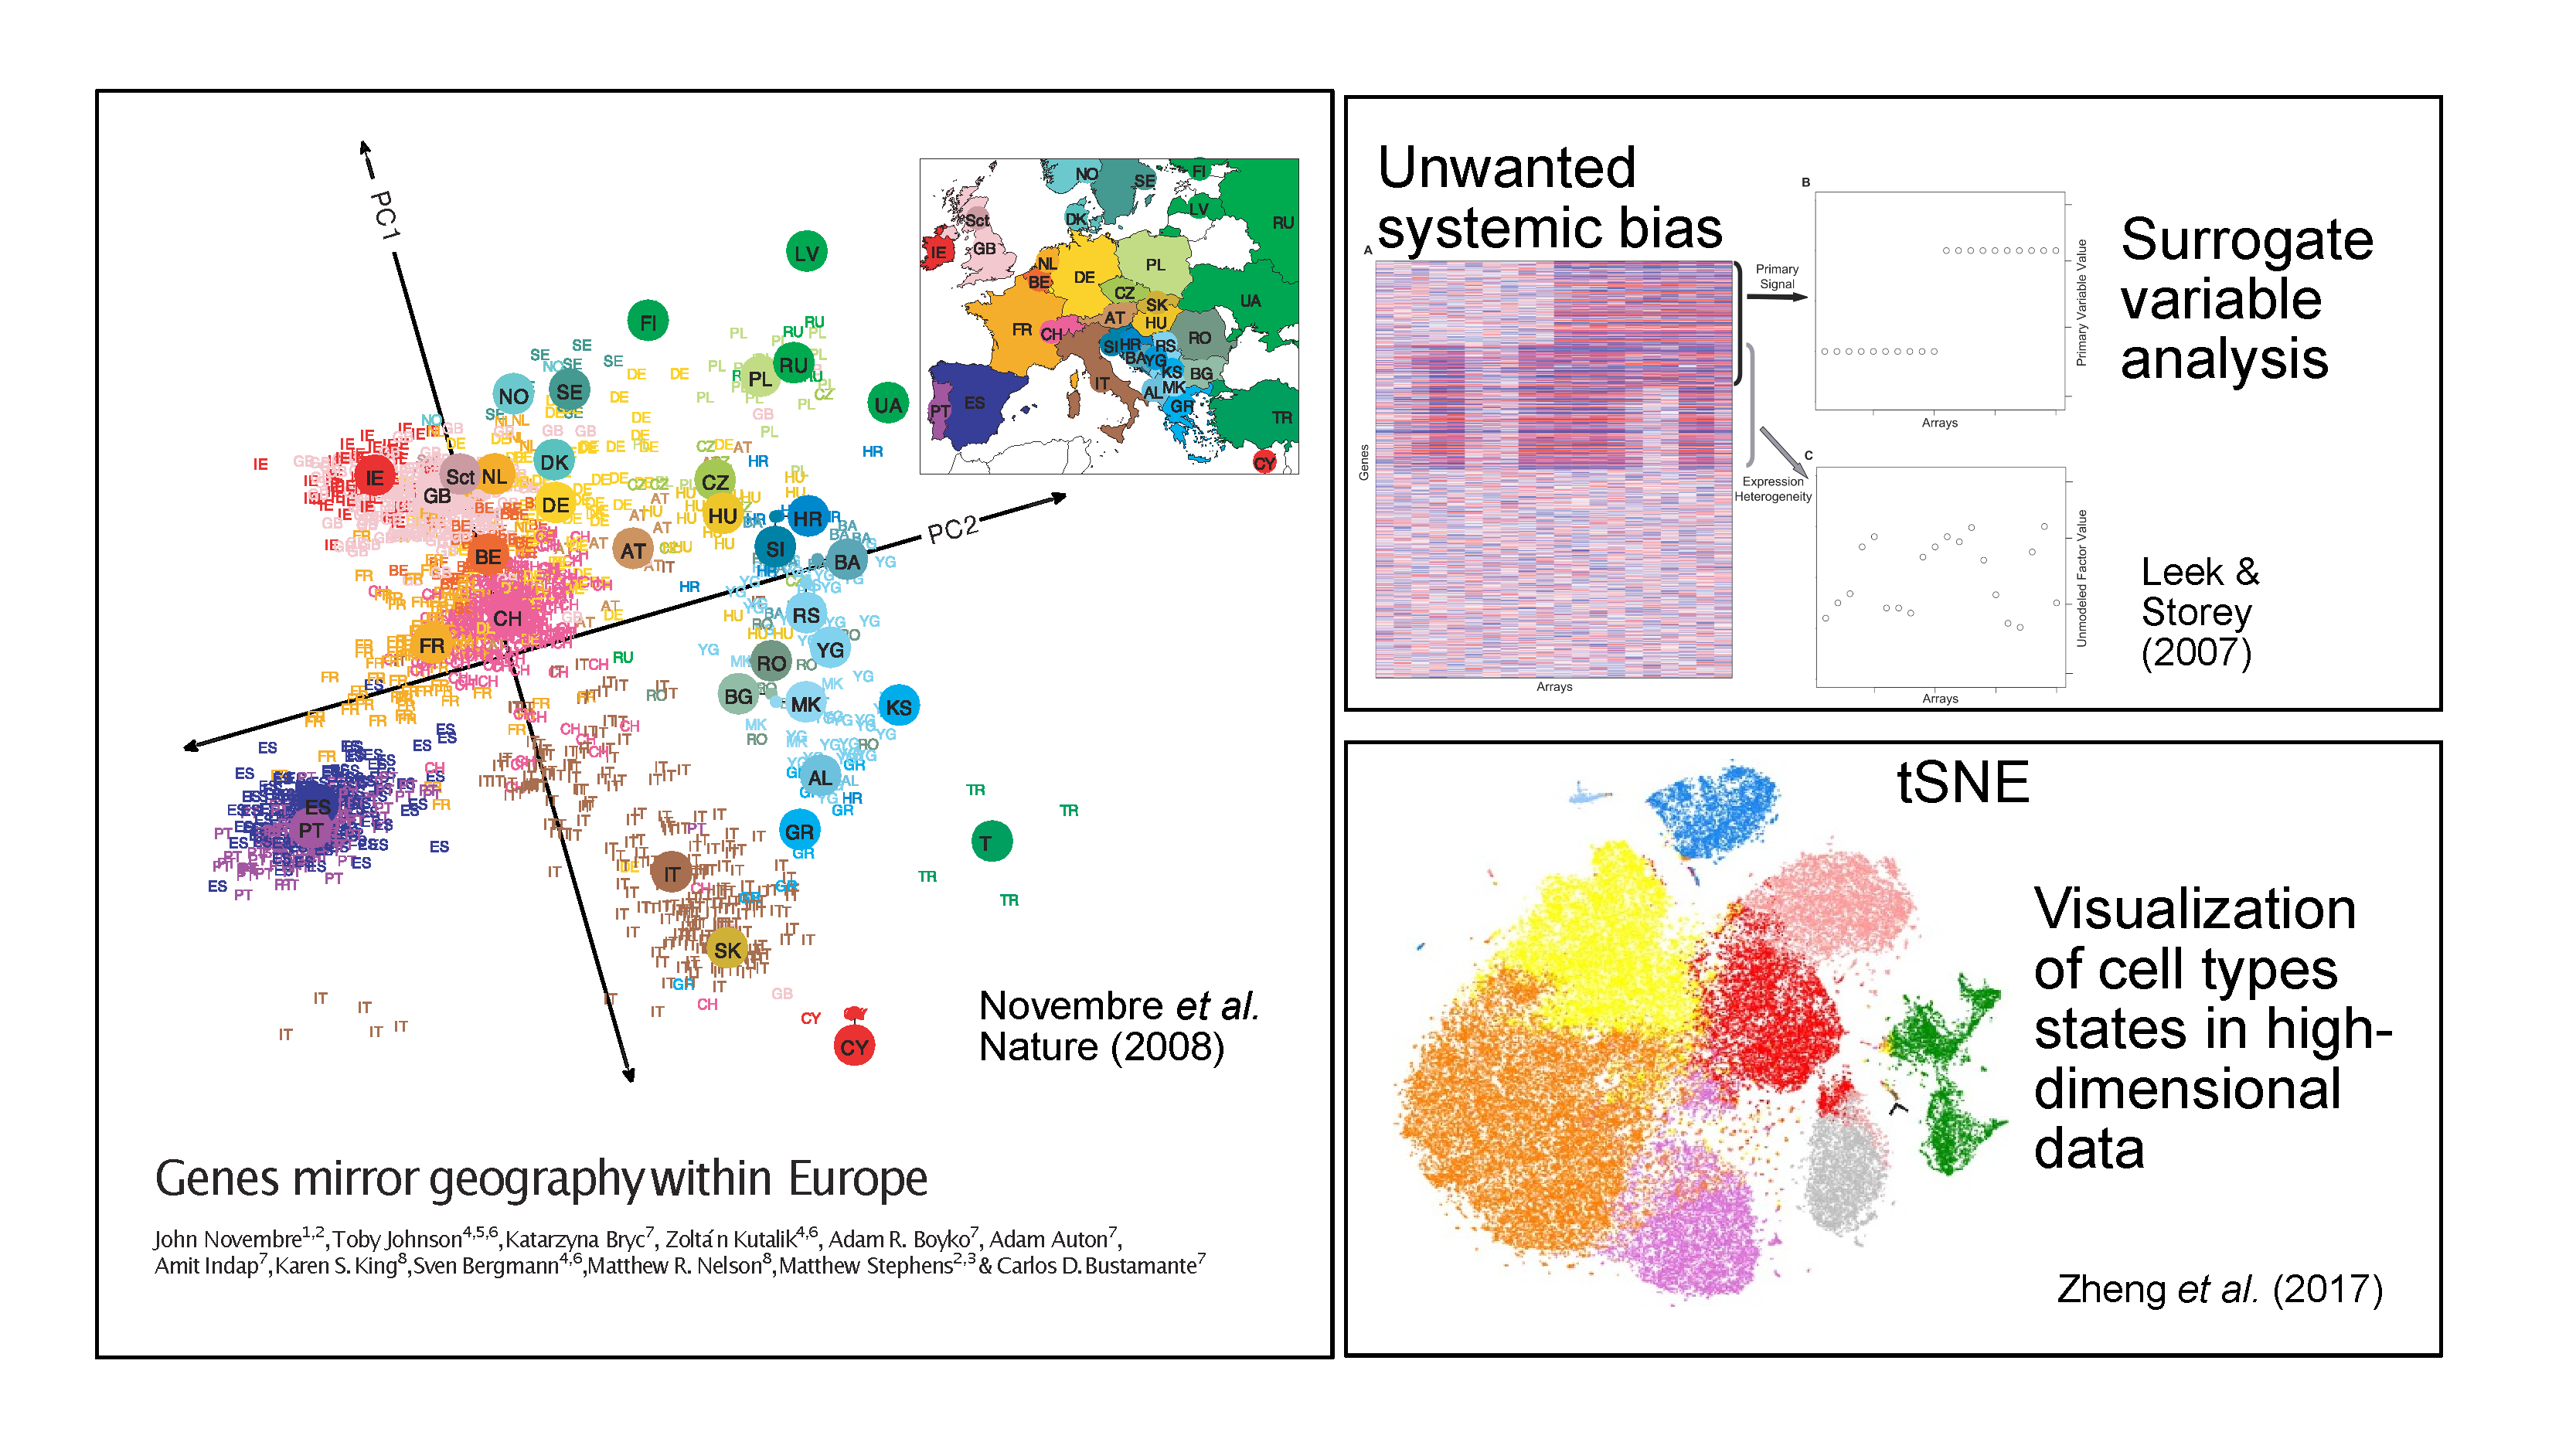
\includegraphics{Vis/unsupervised/why_unsupervised_learning.pdf}
\end{frame}

\begin{frame}{Human brain is very good at learning meaningful
representations}
\protect\hypertarget{human-brain-is-very-good-at-learning-meaningful-representations}{}
\scriptsize

\begin{center}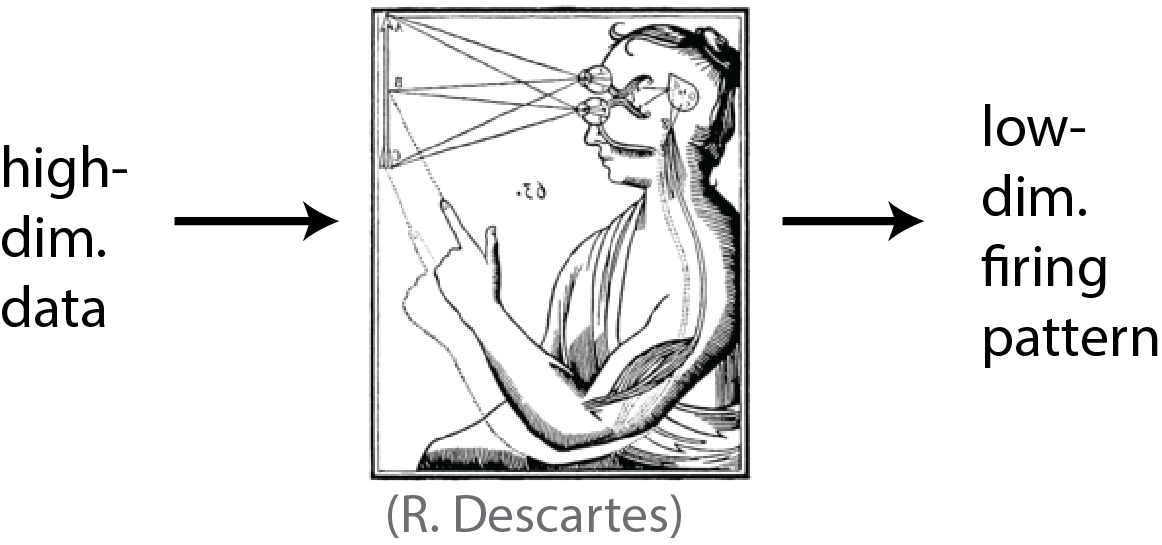
\includegraphics[width=.7\linewidth]{./Vis/unsupervised/descartes} \end{center}

\normalsize
\end{frame}

\begin{frame}{(Digression) Human brain is very good at learning
representations}
\protect\hypertarget{digression-human-brain-is-very-good-at-learning-representations}{}
\begin{columns}[T]
\begin{column}{.65\textwidth}
\scriptsize

\begin{center}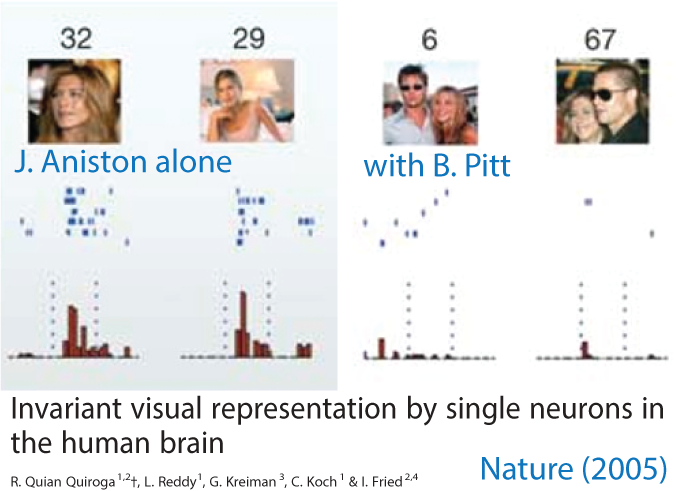
\includegraphics[width=\linewidth]{./Vis/unsupervised/neuron_firing_celebrity} \end{center}

\normalsize
\end{column}

\begin{column}{.3\textwidth}
\begin{itemize}
\item
  \emph{Warning: just an example of some people's brain}
\item
  \emph{The authors also claimed that they found other very specific
  neurons (Halle Berry, Sydney Opera House).}
\end{itemize}
\end{column}
\end{columns}
\end{frame}

\begin{frame}{Can you teach a computer to find useful patterns?}
\protect\hypertarget{can-you-teach-a-computer-to-find-useful-patterns}{}
\scriptsize

\begin{center}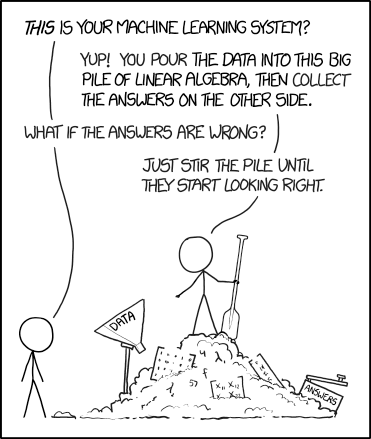
\includegraphics[width=.35\linewidth]{Vis/unsupervised/machine_learning} \end{center}

\normalsize

\tiny

From XKCD
\end{frame}

\begin{frame}{Two strategies to learn a ``good'' representation}
\protect\hypertarget{two-strategies-to-learn-a-good-representation}{}
\begin{columns}[T]
\begin{column}{.45\textwidth}
\begin{block}{Feature engineering}
\protect\hypertarget{feature-engineering}{}
Construct useful combinations of variables, feature engineering

\begin{itemize}
\item
  Principal component analysis (matrix factorization)
\item
  Pattern recognition
\item
  Clustering (average patterns \(\approx\) combined features/data)
\end{itemize}
\end{block}
\end{column}

\begin{column}{.45\textwidth}
\begin{block}{Manifold learning}
\protect\hypertarget{manifold-learning}{}
Change the manifold (a coordinate system) of data

\begin{itemize}
\item
  Probabilistic topic models: word frequency \(\to\) simplex
\item
  Angular space \(\to\) Euclidean space
\item
  Observed high-dim. \(\to\) interpretable ones
\end{itemize}
\end{block}
\end{column}
\end{columns}

We use both strategies in practice.
\end{frame}

\begin{frame}{Feature engineering combines multiple vars. to a
``factor'' var.}
\protect\hypertarget{feature-engineering-combines-multiple-vars.-to-a-factor-var.}{}
\begin{columns}[T]
\begin{column}{.5\textwidth}
\scriptsize

\normalsize

\scriptsize

\normalsize

\[\mathbf{x}_{i} = \mathbf{u}_{i} V^{\top} + \mathcal{N}\!\left(\mathbf{0},I\right)\]

\scriptsize

\normalsize

\scriptsize

\onslide<1->{


\begin{center}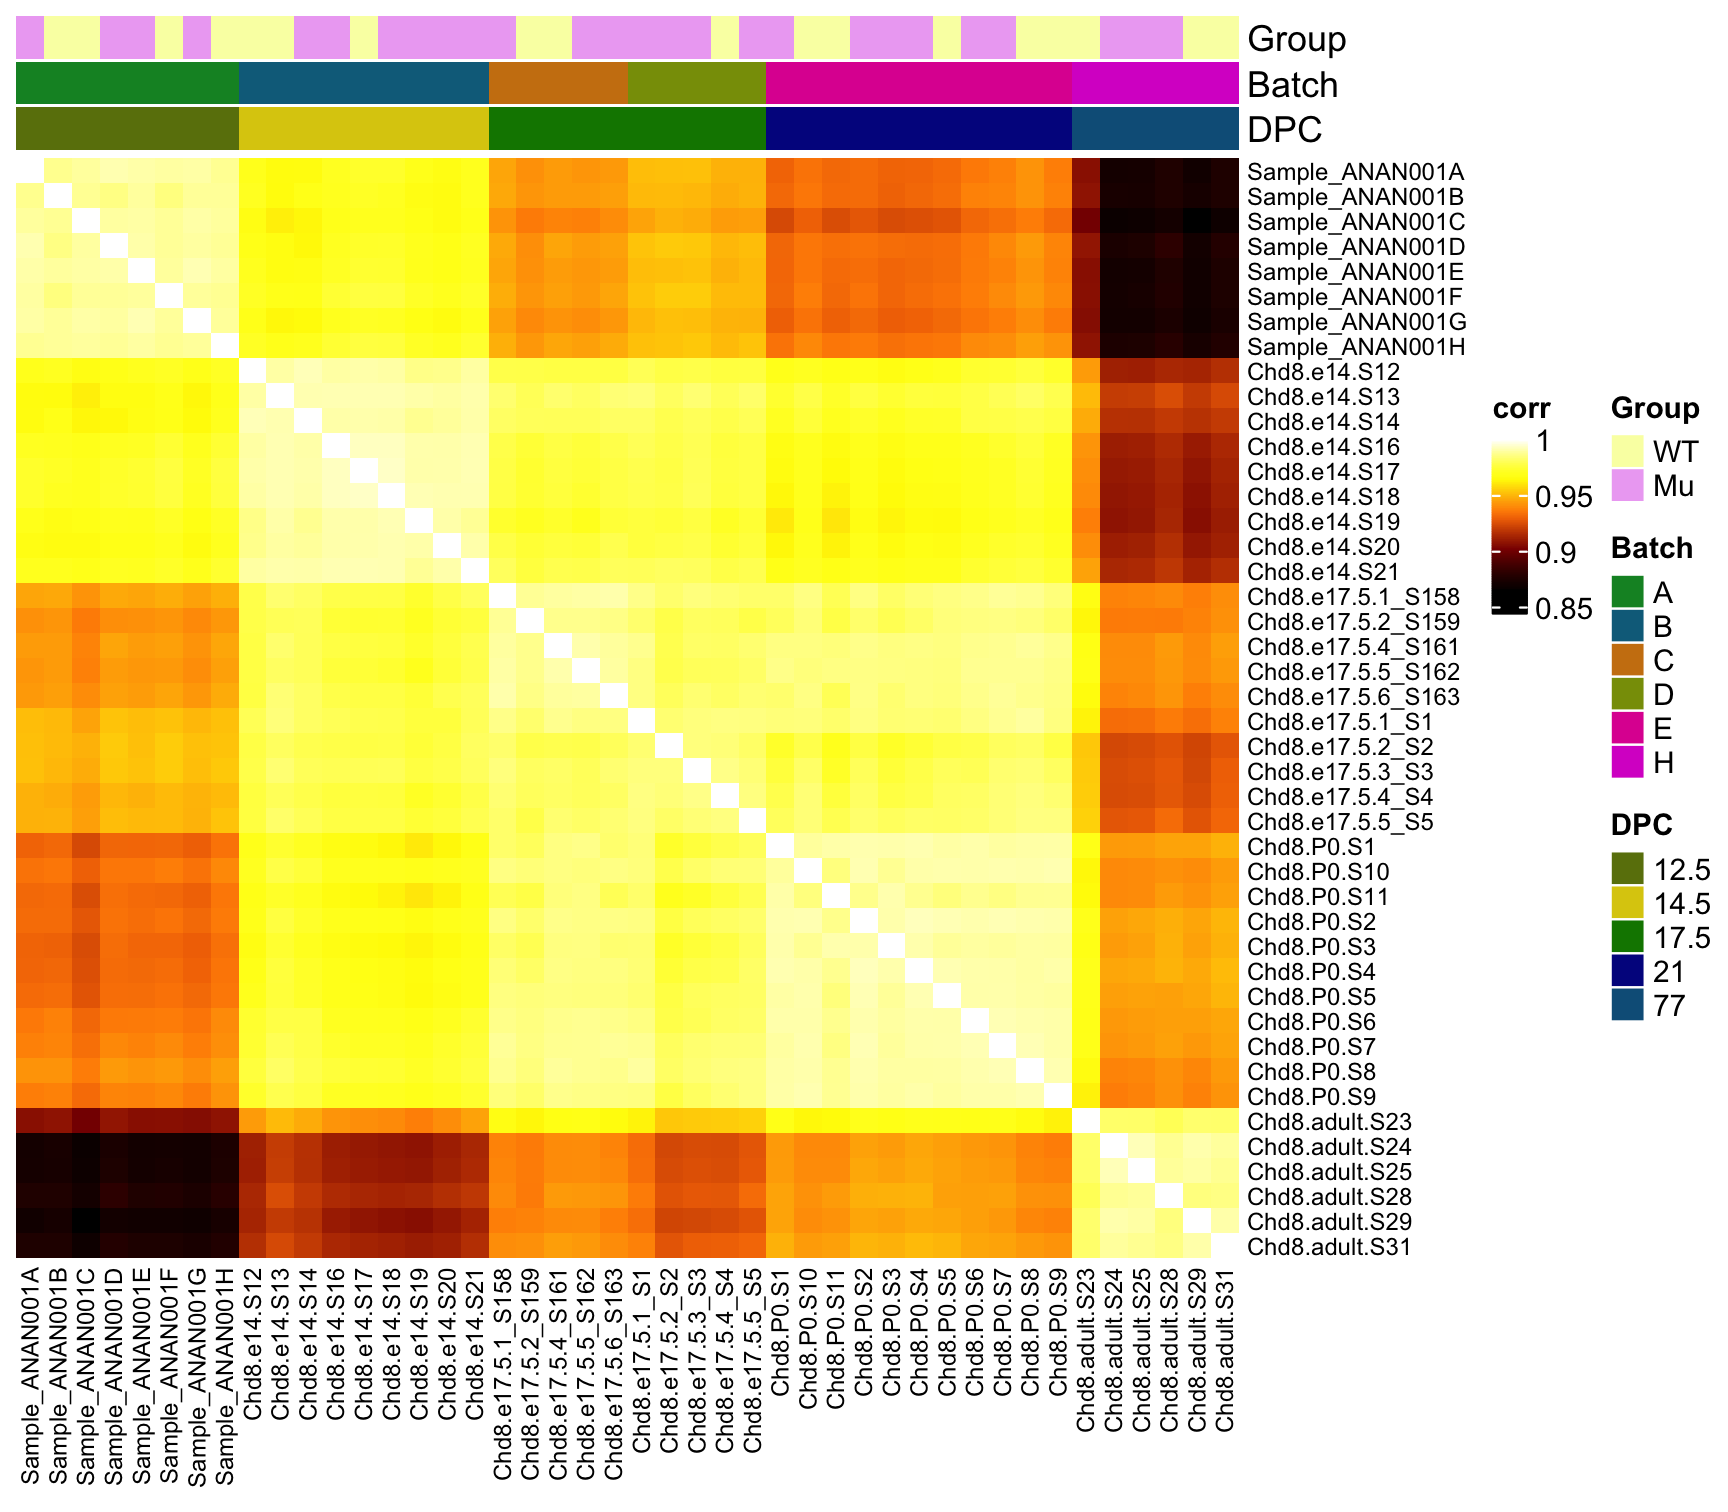
\includegraphics{Fig/unsupervised/unnamed-chunk-8-1} \end{center}


}

\normalsize
\end{column}

\begin{column}{.5\textwidth}
\scriptsize

\normalsize

\scriptsize

\only<2>{


\begin{center}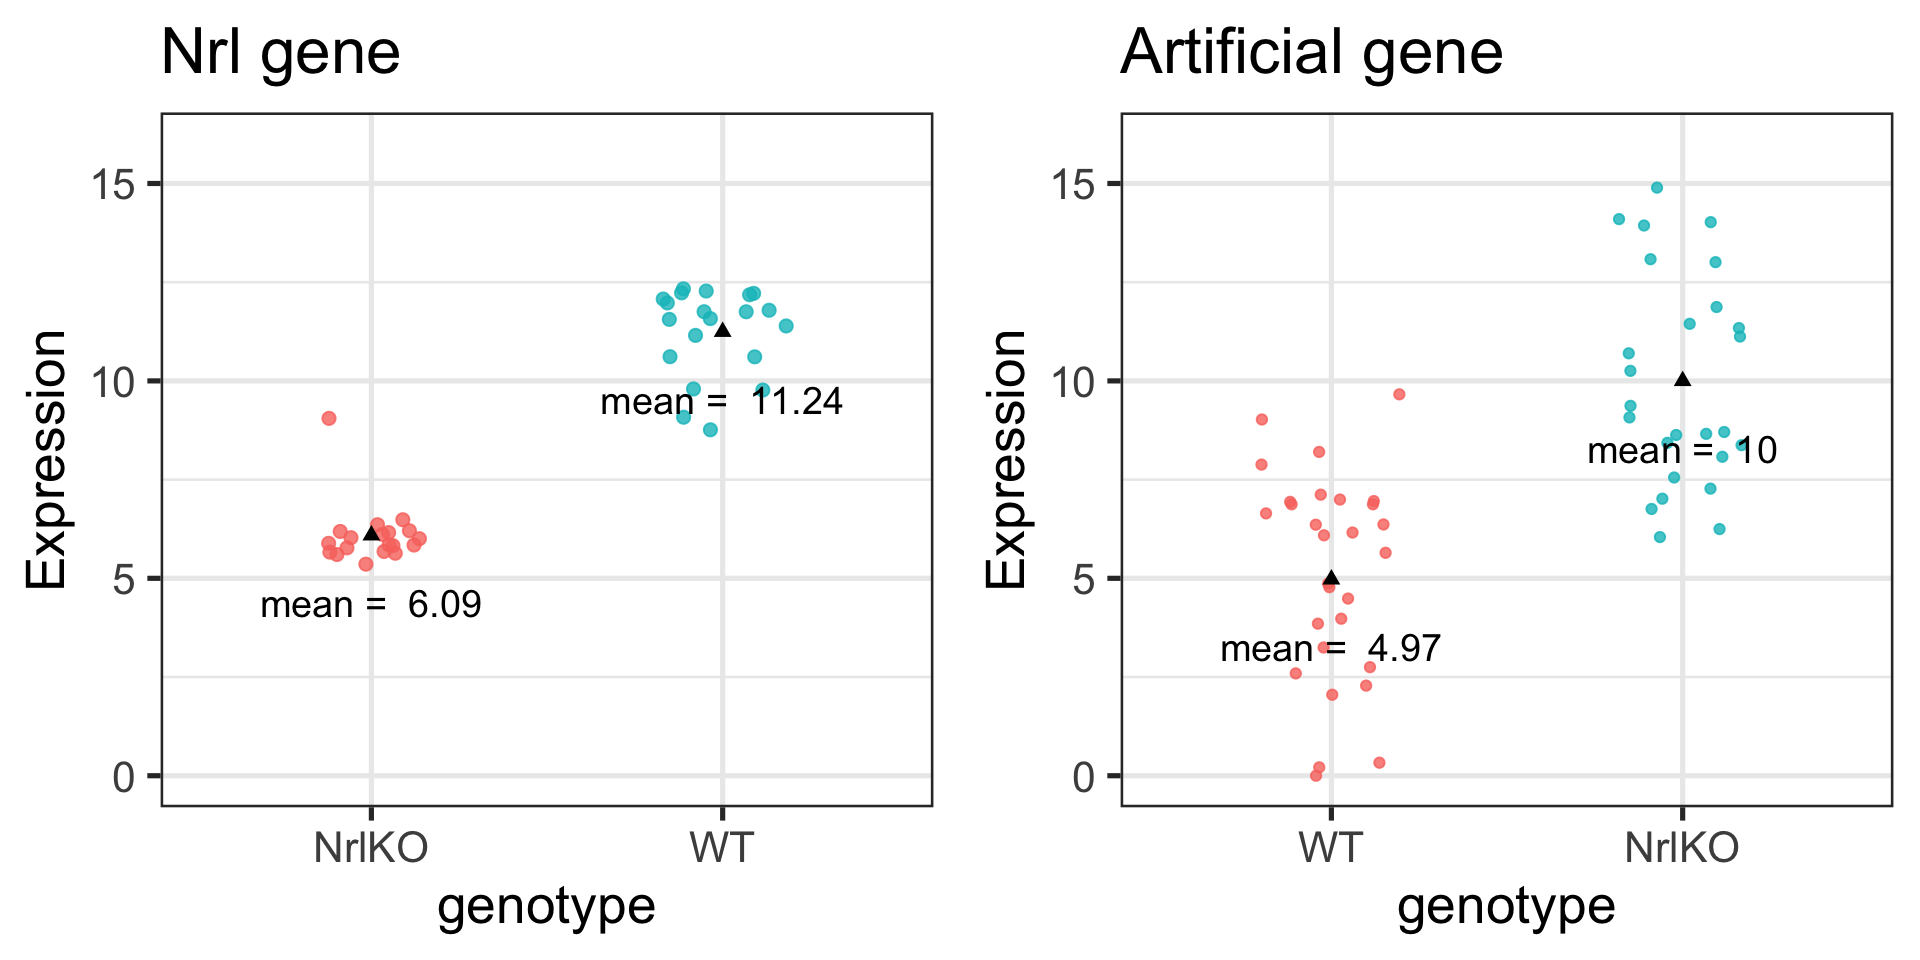
\includegraphics{Fig/unsupervised/unnamed-chunk-10-1} \end{center}


}

\normalsize
\end{column}
\end{columns}
\end{frame}

\begin{frame}{Feature engineering}
\protect\hypertarget{feature-engineering-1}{}
\begin{columns}[T]
\begin{column}{.5\textwidth}
\[\mathbf{x}_{i} = \mathbf{u}_{i} V^{\top} + \mathcal{N}\!\left(\mathbf{0},I\right)\]

\begin{itemize}
\item
  We call each column of U and \(V\) a factor (row/column)
\item
  One factor corresponds to the activities/patterns/expressions of 100
  genes/samples
\item
  We will discuss further later.
\end{itemize}
\end{column}

\begin{column}{.5\textwidth}
\scriptsize

\begin{center}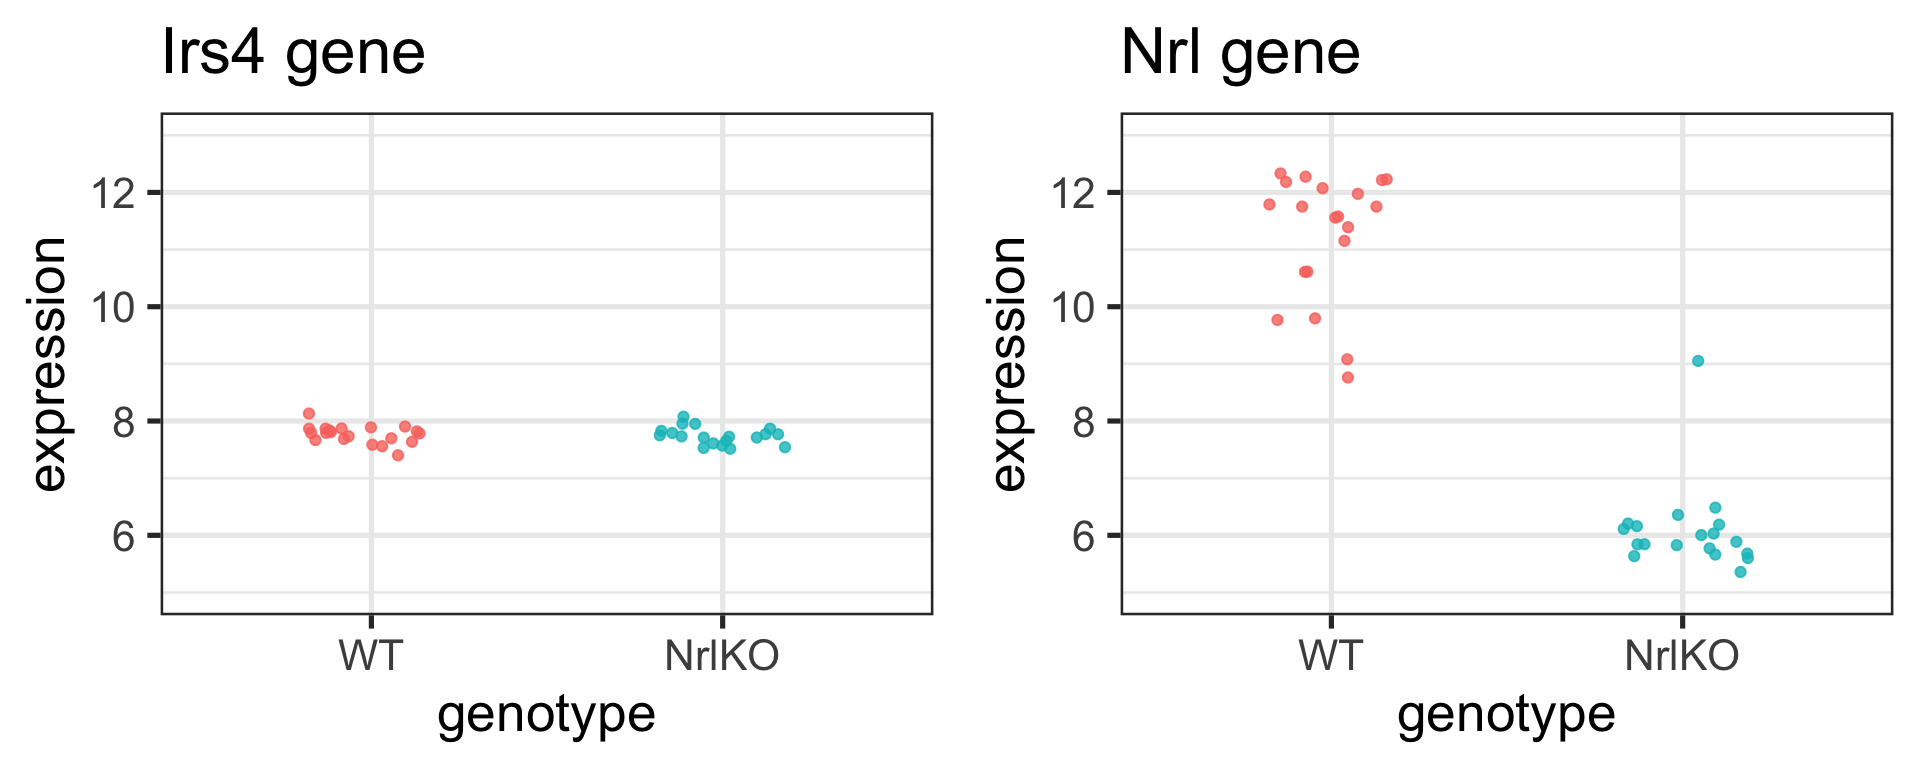
\includegraphics{Fig/unsupervised/unnamed-chunk-11-1} \end{center}

\normalsize
\end{column}
\end{columns}
\end{frame}

\begin{frame}{Manifold learning transforms the coordinate system of
data}
\protect\hypertarget{manifold-learning-transforms-the-coordinate-system-of-data}{}
\begin{columns}[T]
\begin{column}{.5\textwidth}
\scriptsize

\normalsize

\scriptsize

\only<1>{


\begin{center}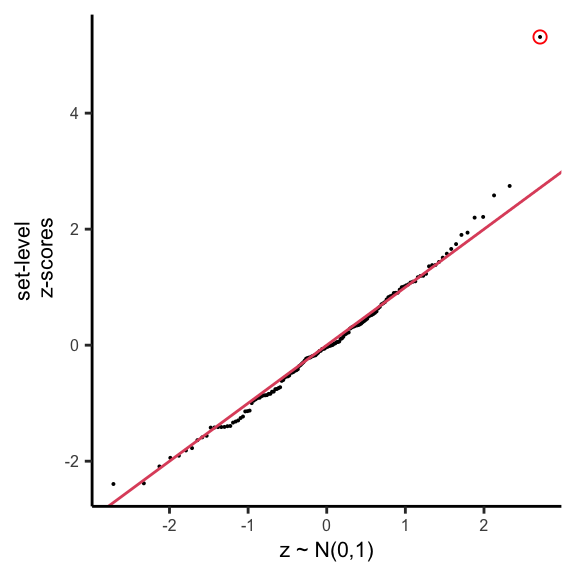
\includegraphics{Fig/unsupervised/unnamed-chunk-13-1} \end{center}


}

\normalsize

\scriptsize

\onslide<2->{


\begin{center}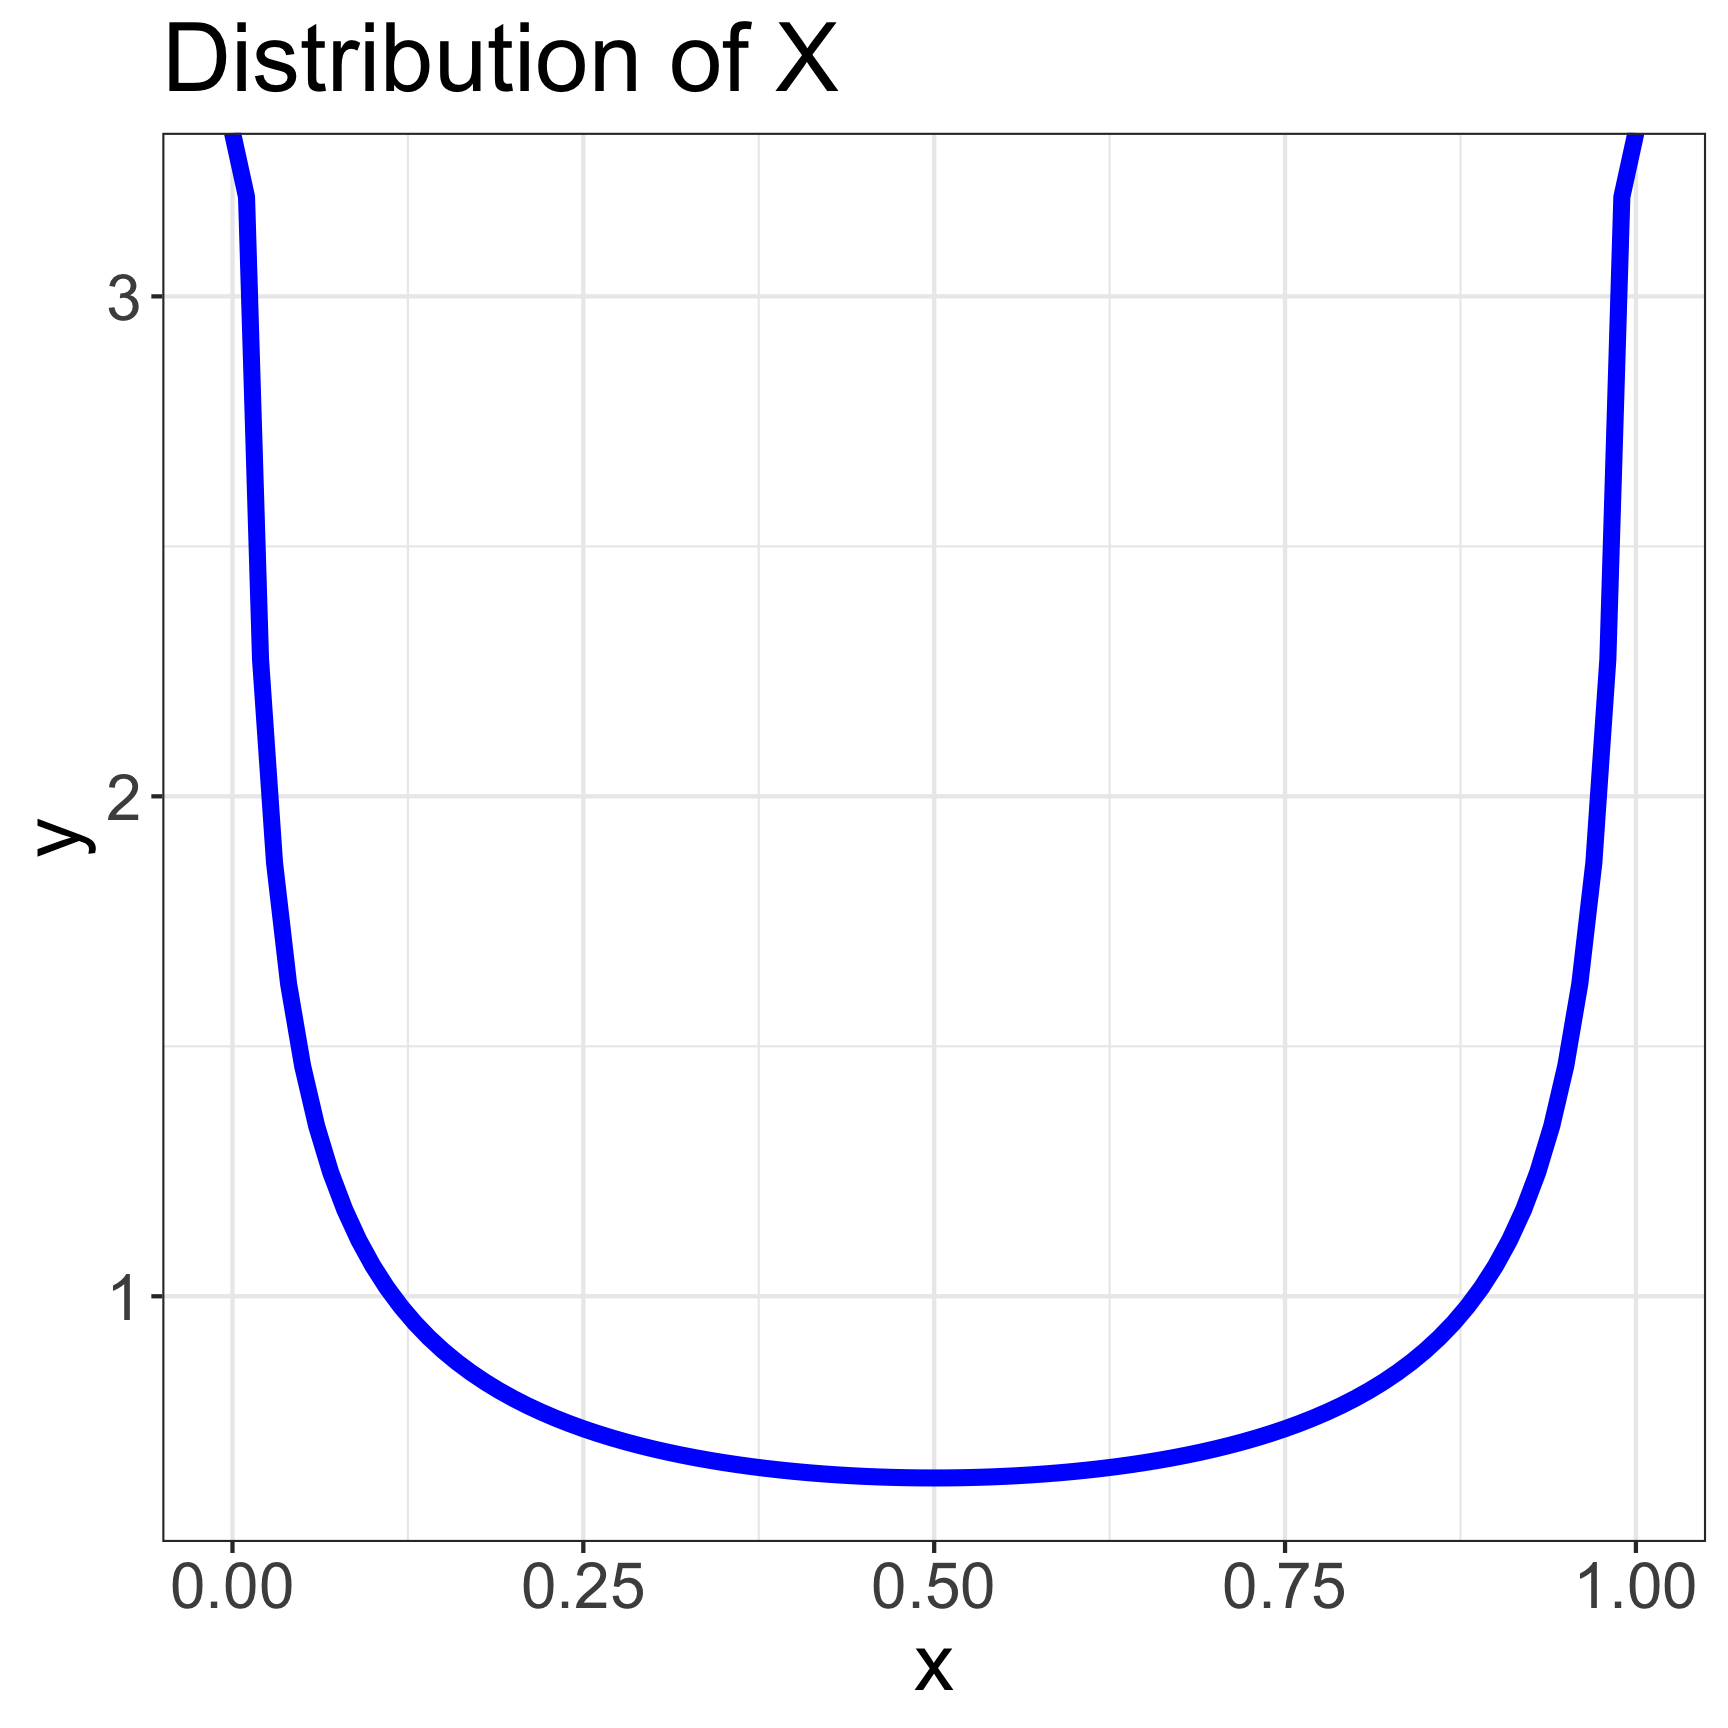
\includegraphics{Fig/unsupervised/unnamed-chunk-14-1} \end{center}


}

\normalsize

\begin{itemize}
\tightlist
\item
  \(x^{2} + y^{2} + z^{2} = 1\)
\end{itemize}

\tiny

\begin{itemize}
\tightlist
\item
  Data from \url{https://simplemaps.com/data/world-cities}
\end{itemize}
\end{column}

\begin{column}{.5\textwidth}
\scriptsize

\normalsize

\scriptsize

\only<3>{


\begin{center}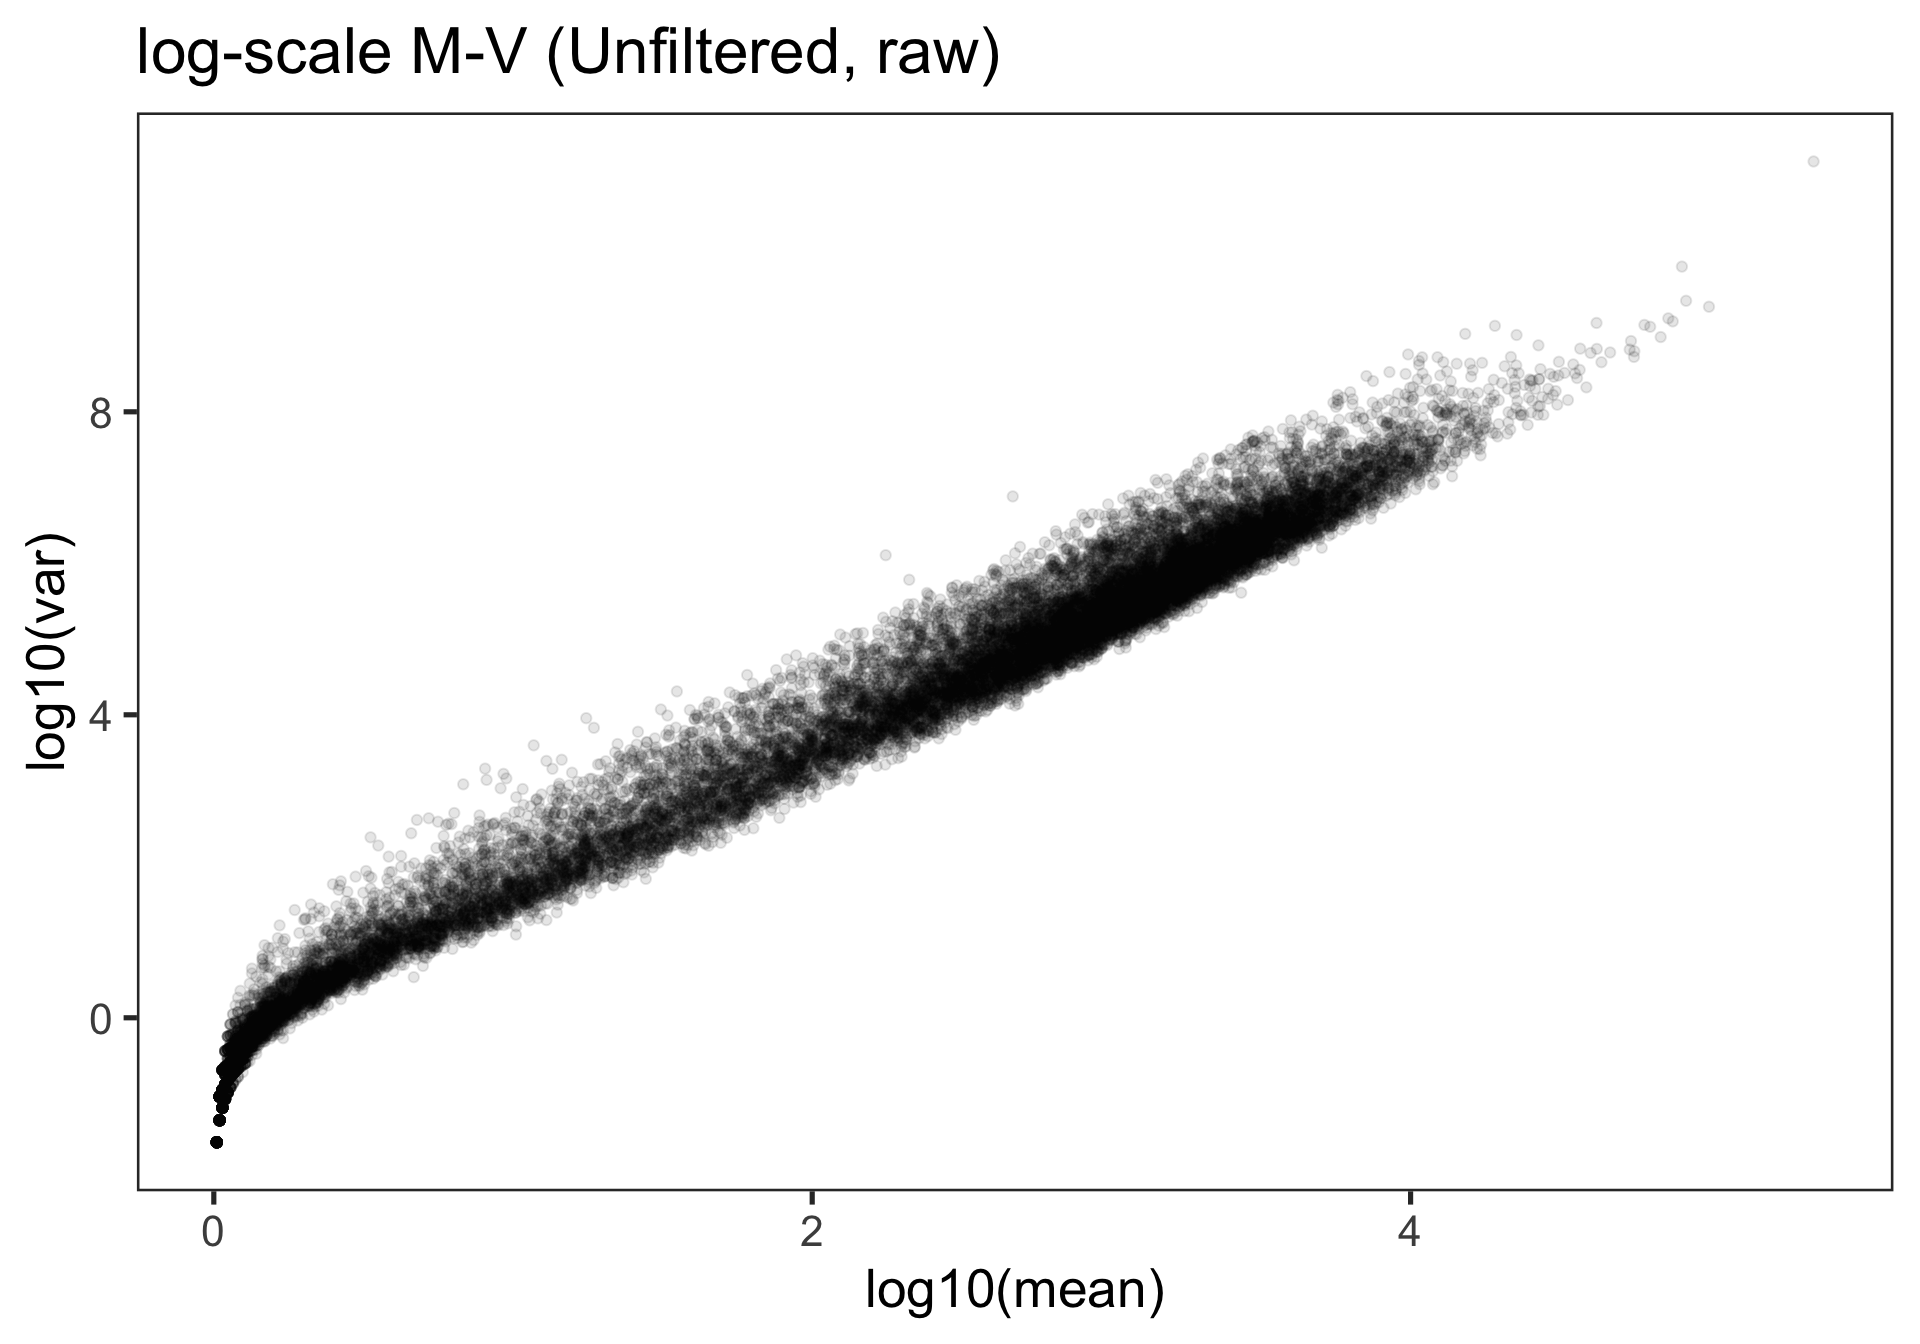
\includegraphics{Fig/unsupervised/unnamed-chunk-16-1} \end{center}


}

\normalsize

\scriptsize

\only<4>{


\begin{center}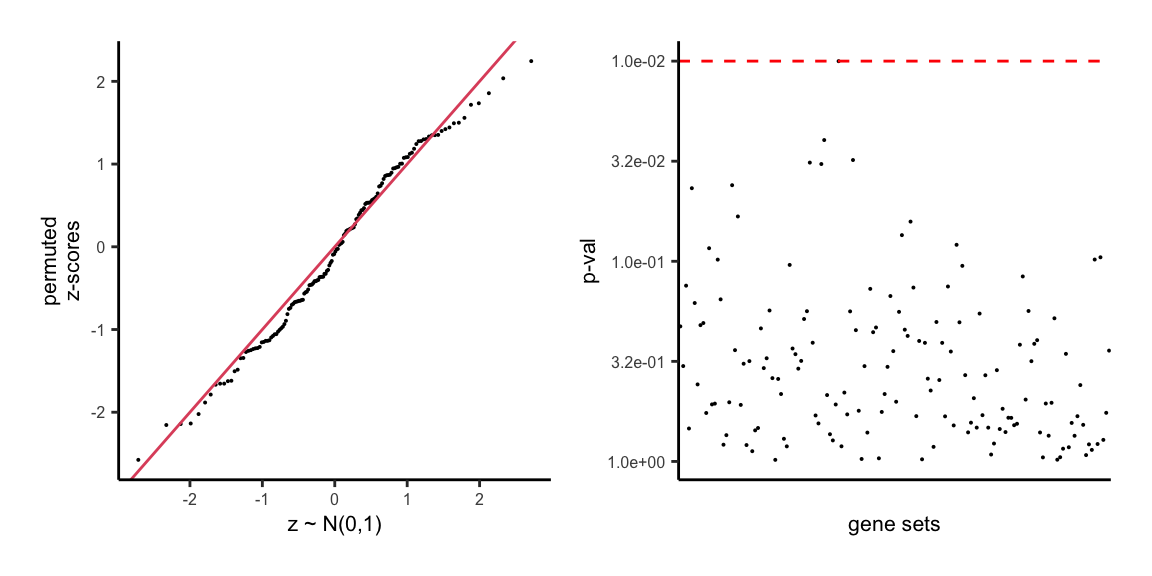
\includegraphics{Fig/unsupervised/unnamed-chunk-17-1} \end{center}


}

\normalsize

\scriptsize

\only<5>{


\begin{center}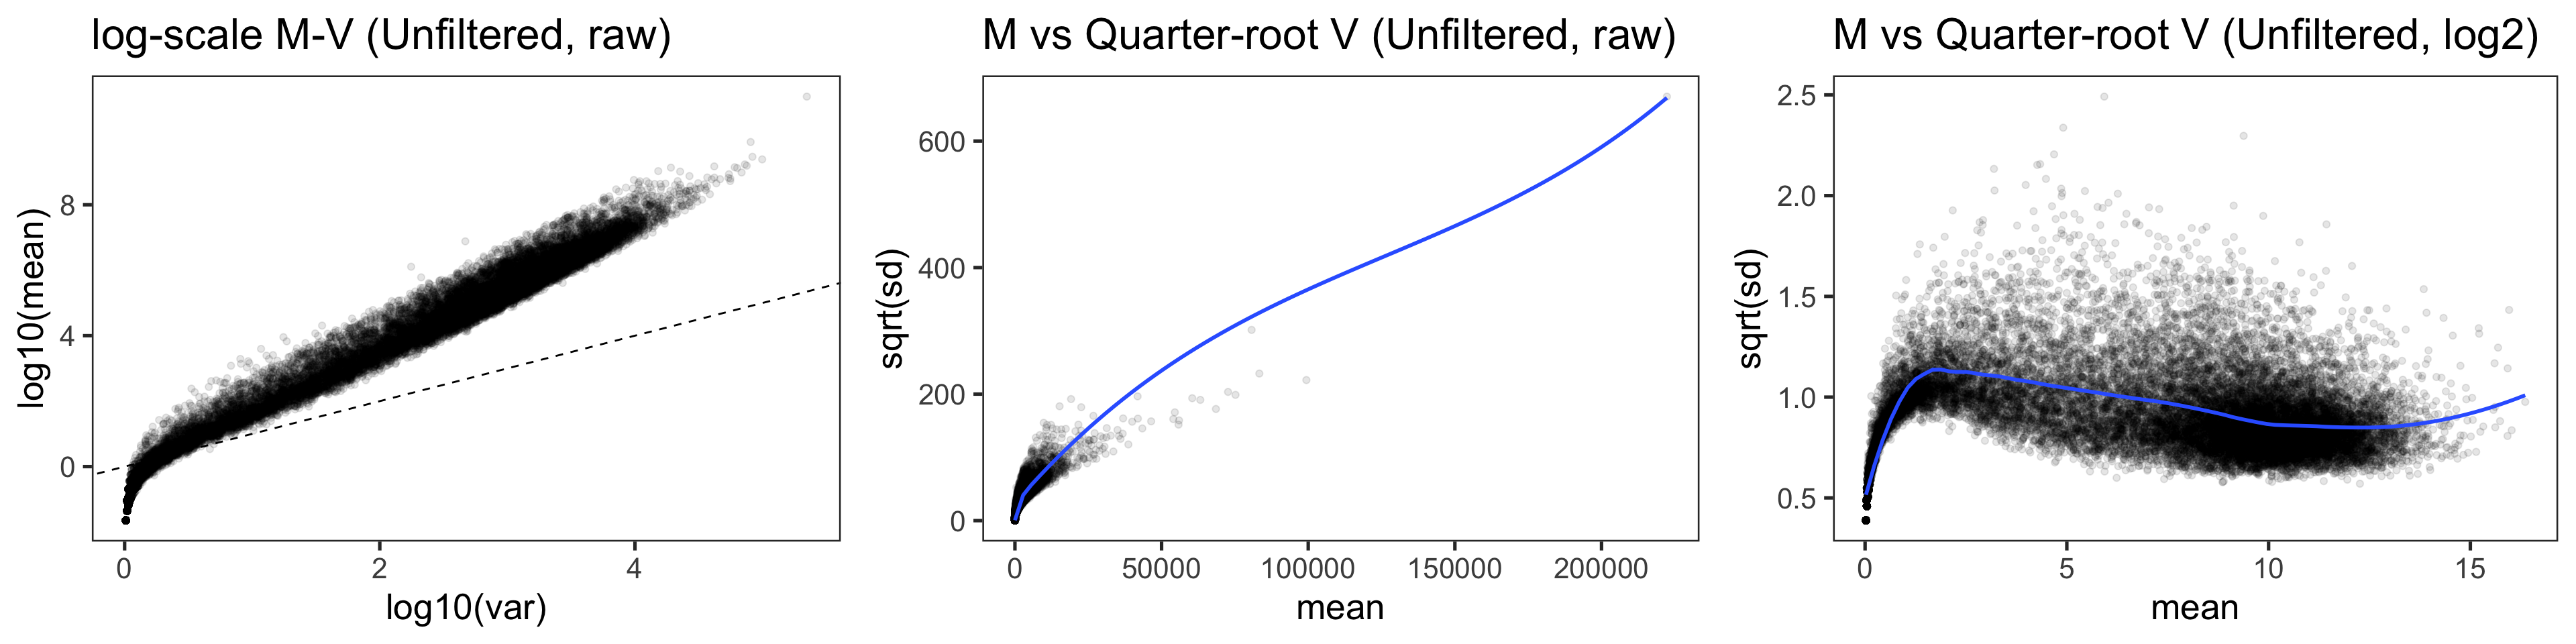
\includegraphics{Fig/unsupervised/unnamed-chunk-18-1} \end{center}


}

\normalsize
\end{column}
\end{columns}
\end{frame}

\begin{frame}{Representation learning}
\protect\hypertarget{representation-learning}{}
\begin{columns}[T]
\begin{column}{.45\textwidth}
\begin{block}{Feature engineering}
\protect\hypertarget{feature-engineering-2}{}
\begin{itemize}
\item
  Combine samples based on similarity to learn common features
\item
  Combine features/genes/proteins to create a new factor
\item
  Matrix factorization to capture factors that explain large variation
\end{itemize}
\end{block}
\end{column}

\begin{column}{.45\textwidth}
\begin{block}{Manifold learning}
\protect\hypertarget{manifold-learning-1}{}
\begin{itemize}
\item
  Change the coordinate system
\item
  What's not separable in one space can be spread out in another one
\item
  Apply non-linear functions to a set of features
\end{itemize}
\end{block}
\end{column}
\end{columns}
\end{frame}

\hypertarget{principal-component-analysis}{%
\section{Principal Component
Analysis}\label{principal-component-analysis}}

\begin{frame}[fragile]{Working example: the photoreceptor data
(GSE4051)}
\protect\hypertarget{working-example-the-photoreceptor-data-gse4051}{}
First 100 probes in the data matrix:

\begin{columns}[T]
\begin{column}{.25\textwidth}
\scriptsize

\only<1>{


\begin{center}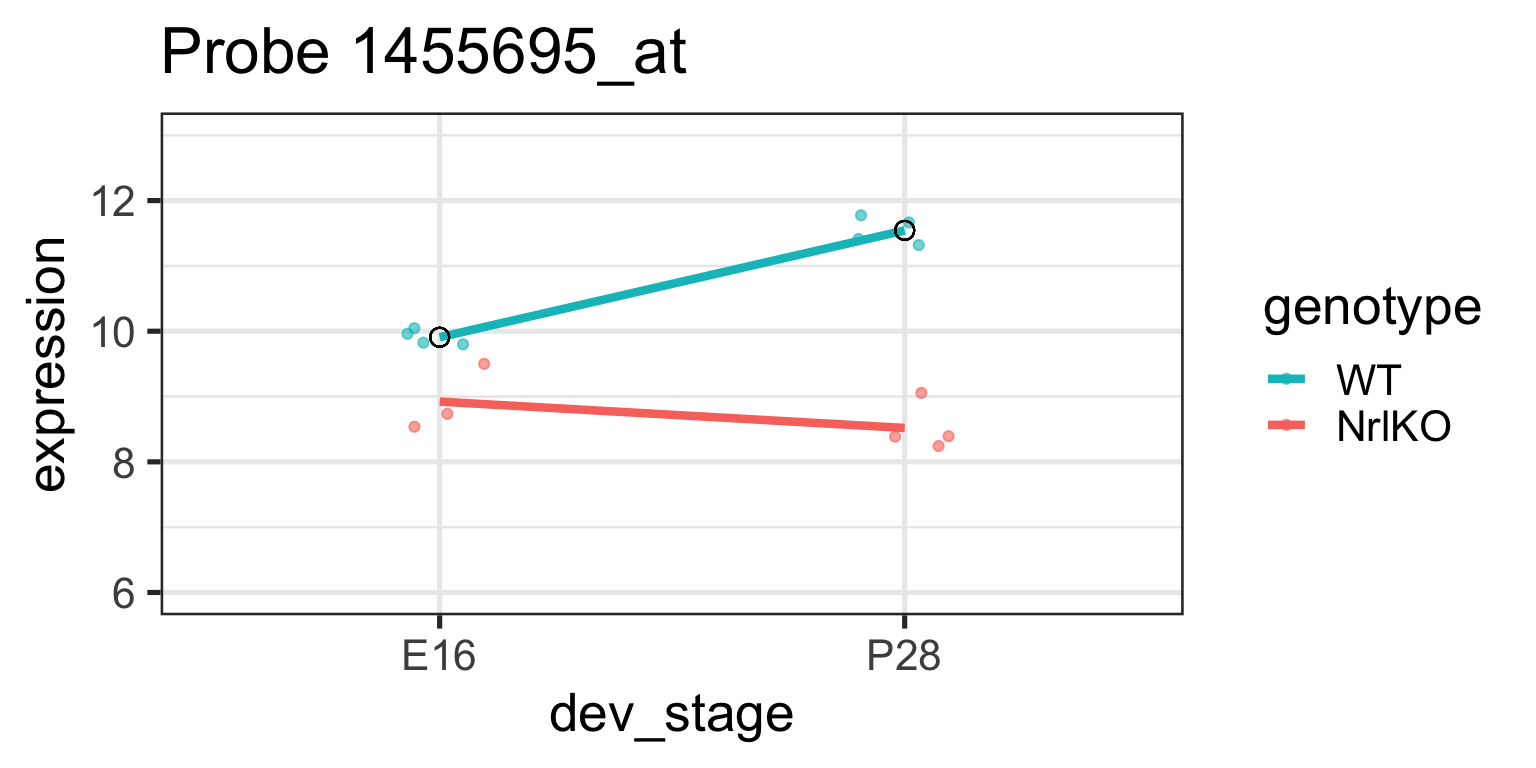
\includegraphics{Fig/unsupervised/unnamed-chunk-20-1} \end{center}


}

\normalsize

\scriptsize

\only<2>{


\begin{center}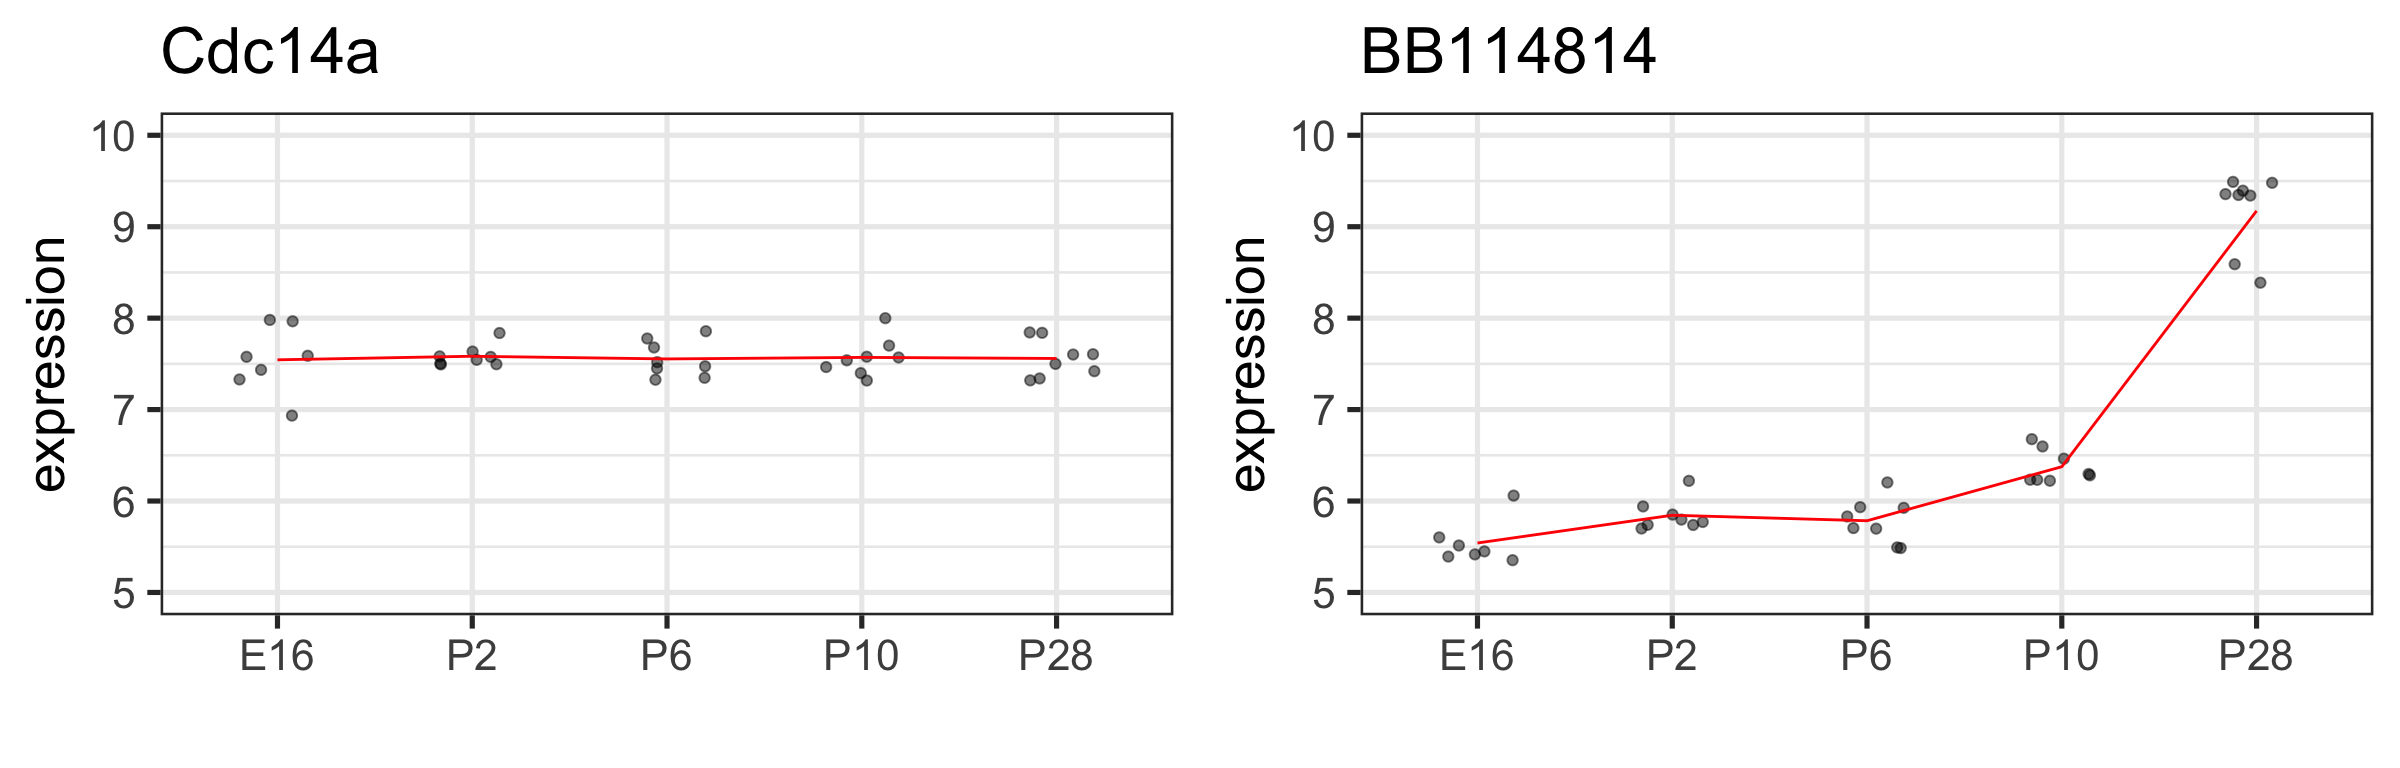
\includegraphics{Fig/unsupervised/unnamed-chunk-21-1} \end{center}


}

\normalsize
\end{column}

\begin{column}{.65\textwidth}
\begin{itemize}
\item
  We will call such a high-dimensional matrix \(X\) (\(m \times n\))
\item
  X has \(m\)=45,101 rows (probes/transcripts/genes/features)
\item
  X has \(n\)=39 columns (samples/\#data points)
\item
  The rows were log-transformed and scaled by \texttt{scale()} for
  visualization
\item
  Each sample is a 45,101-dimensional vector!
\item
  Each gene is a 39-dimensional vector\ldots{}
\end{itemize}
\end{column}
\end{columns}
\end{frame}

\begin{frame}{1-dimensional representations}
\protect\hypertarget{dimensional-representations}{}
\begin{columns}[T]
\begin{column}{.25\textwidth}
First 100 probes:

\scriptsize

\begin{center}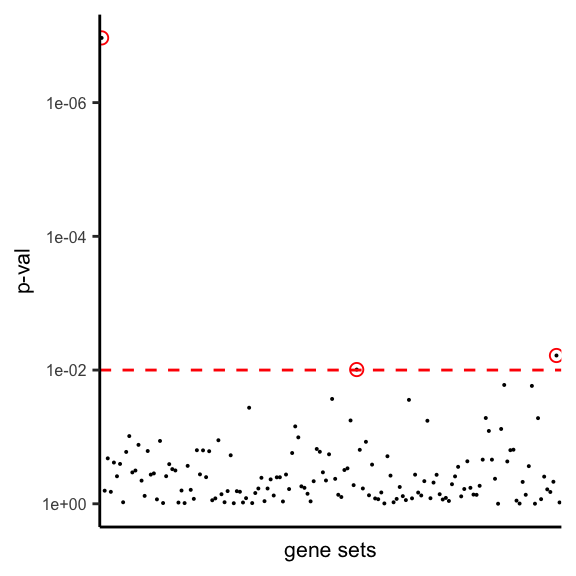
\includegraphics{Fig/unsupervised/unnamed-chunk-22-1} \end{center}

\normalsize
\end{column}

\begin{column}{.65\textwidth}
\scriptsize

\onslide<1->{


\begin{center}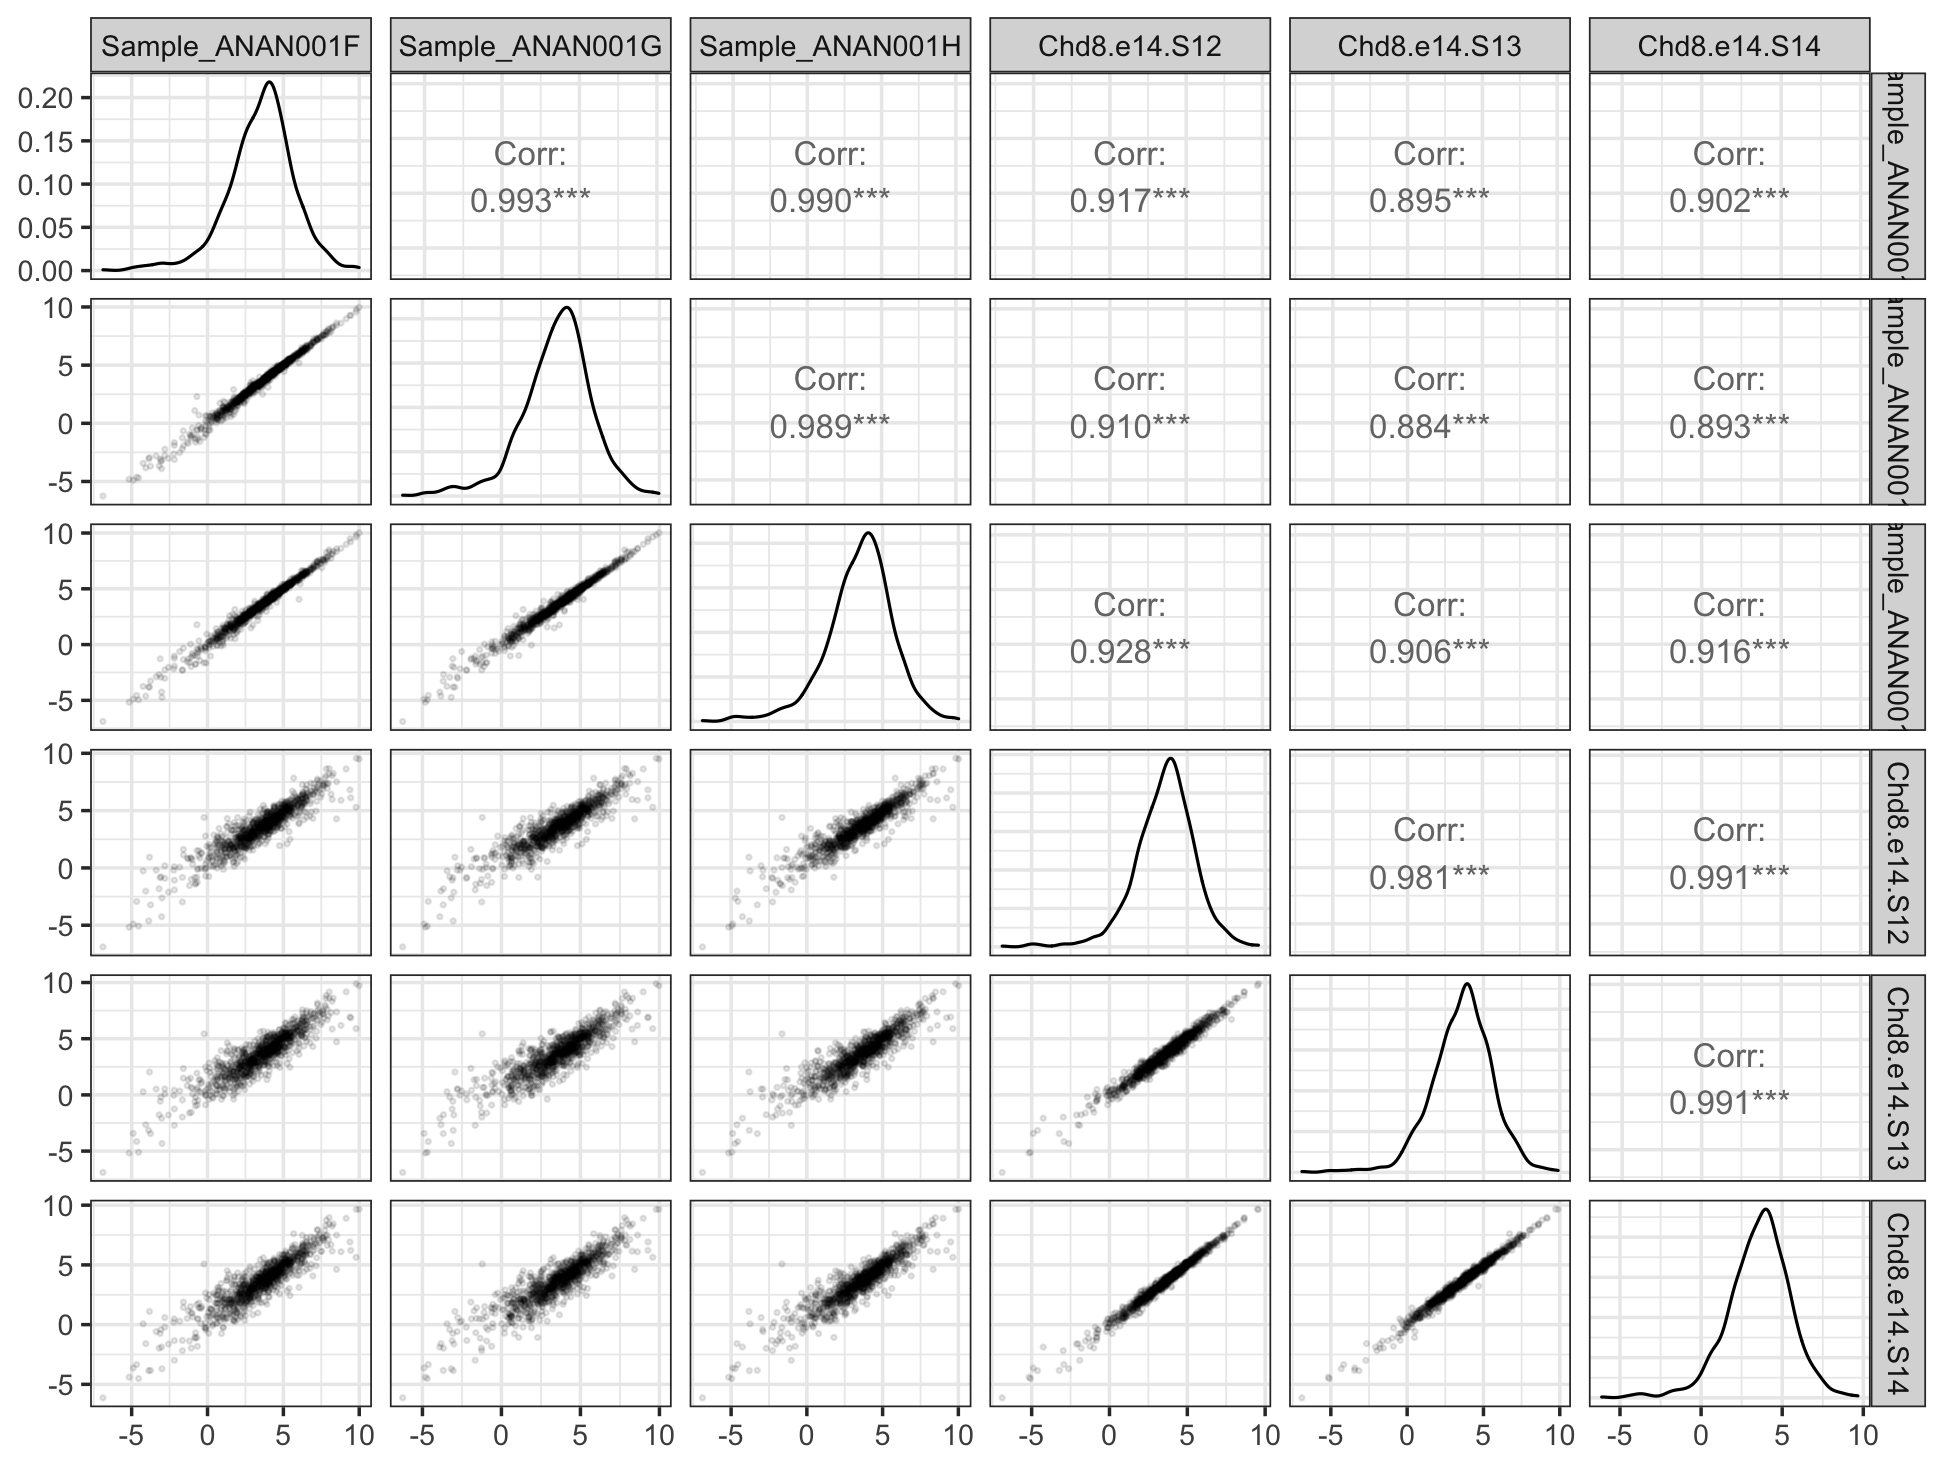
\includegraphics{Fig/unsupervised/unnamed-chunk-23-1} \end{center}


}

\normalsize

\scriptsize

\onslide<2>{


\begin{center}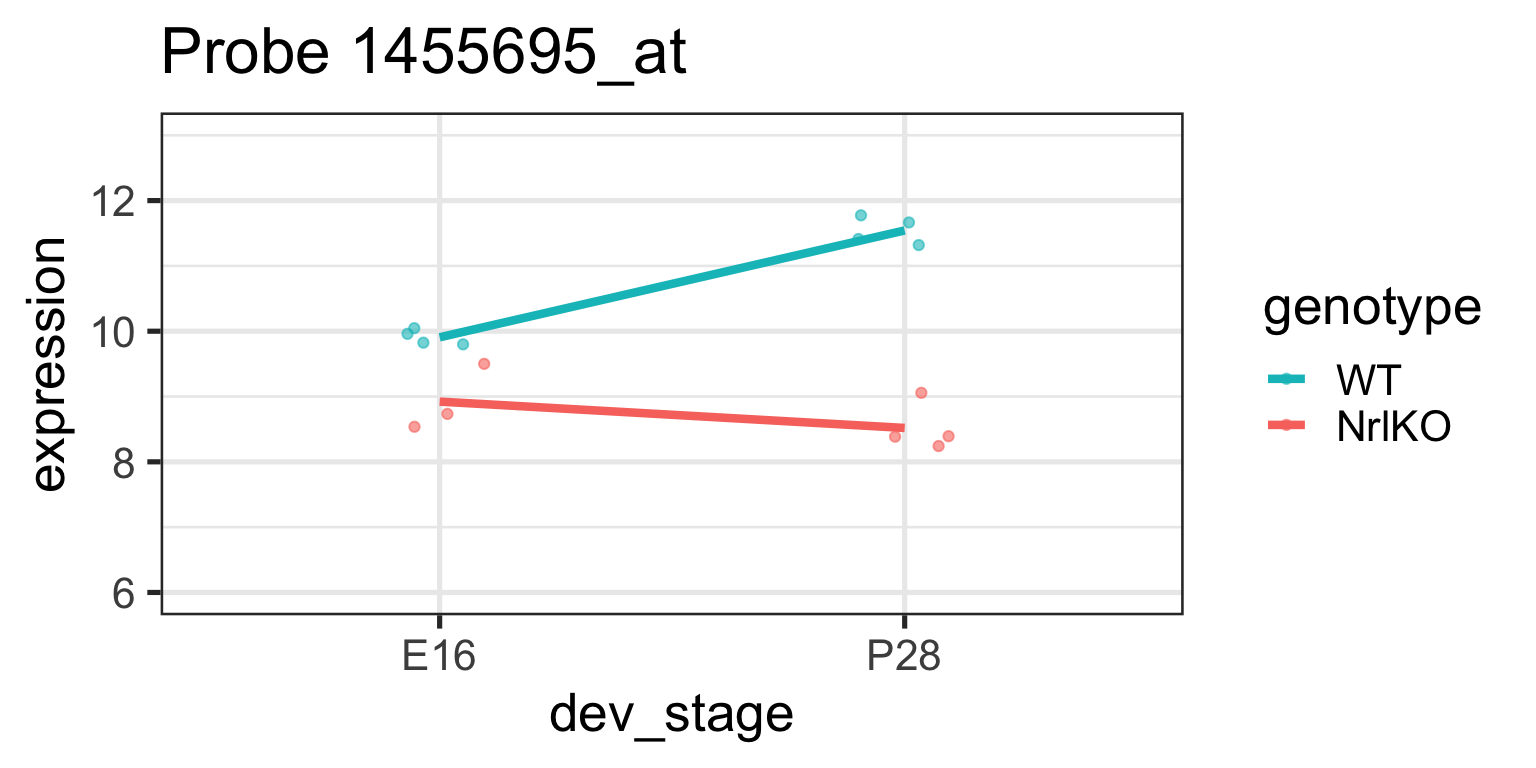
\includegraphics{Fig/unsupervised/unnamed-chunk-24-1} \end{center}


}

\normalsize
\end{column}
\end{columns}
\end{frame}

\begin{frame}{Can you see some common patterns?}
\protect\hypertarget{can-you-see-some-common-patterns}{}
\begin{columns}[T]
\begin{column}{.45\textwidth}
\scriptsize

\onslide<1->{


\begin{center}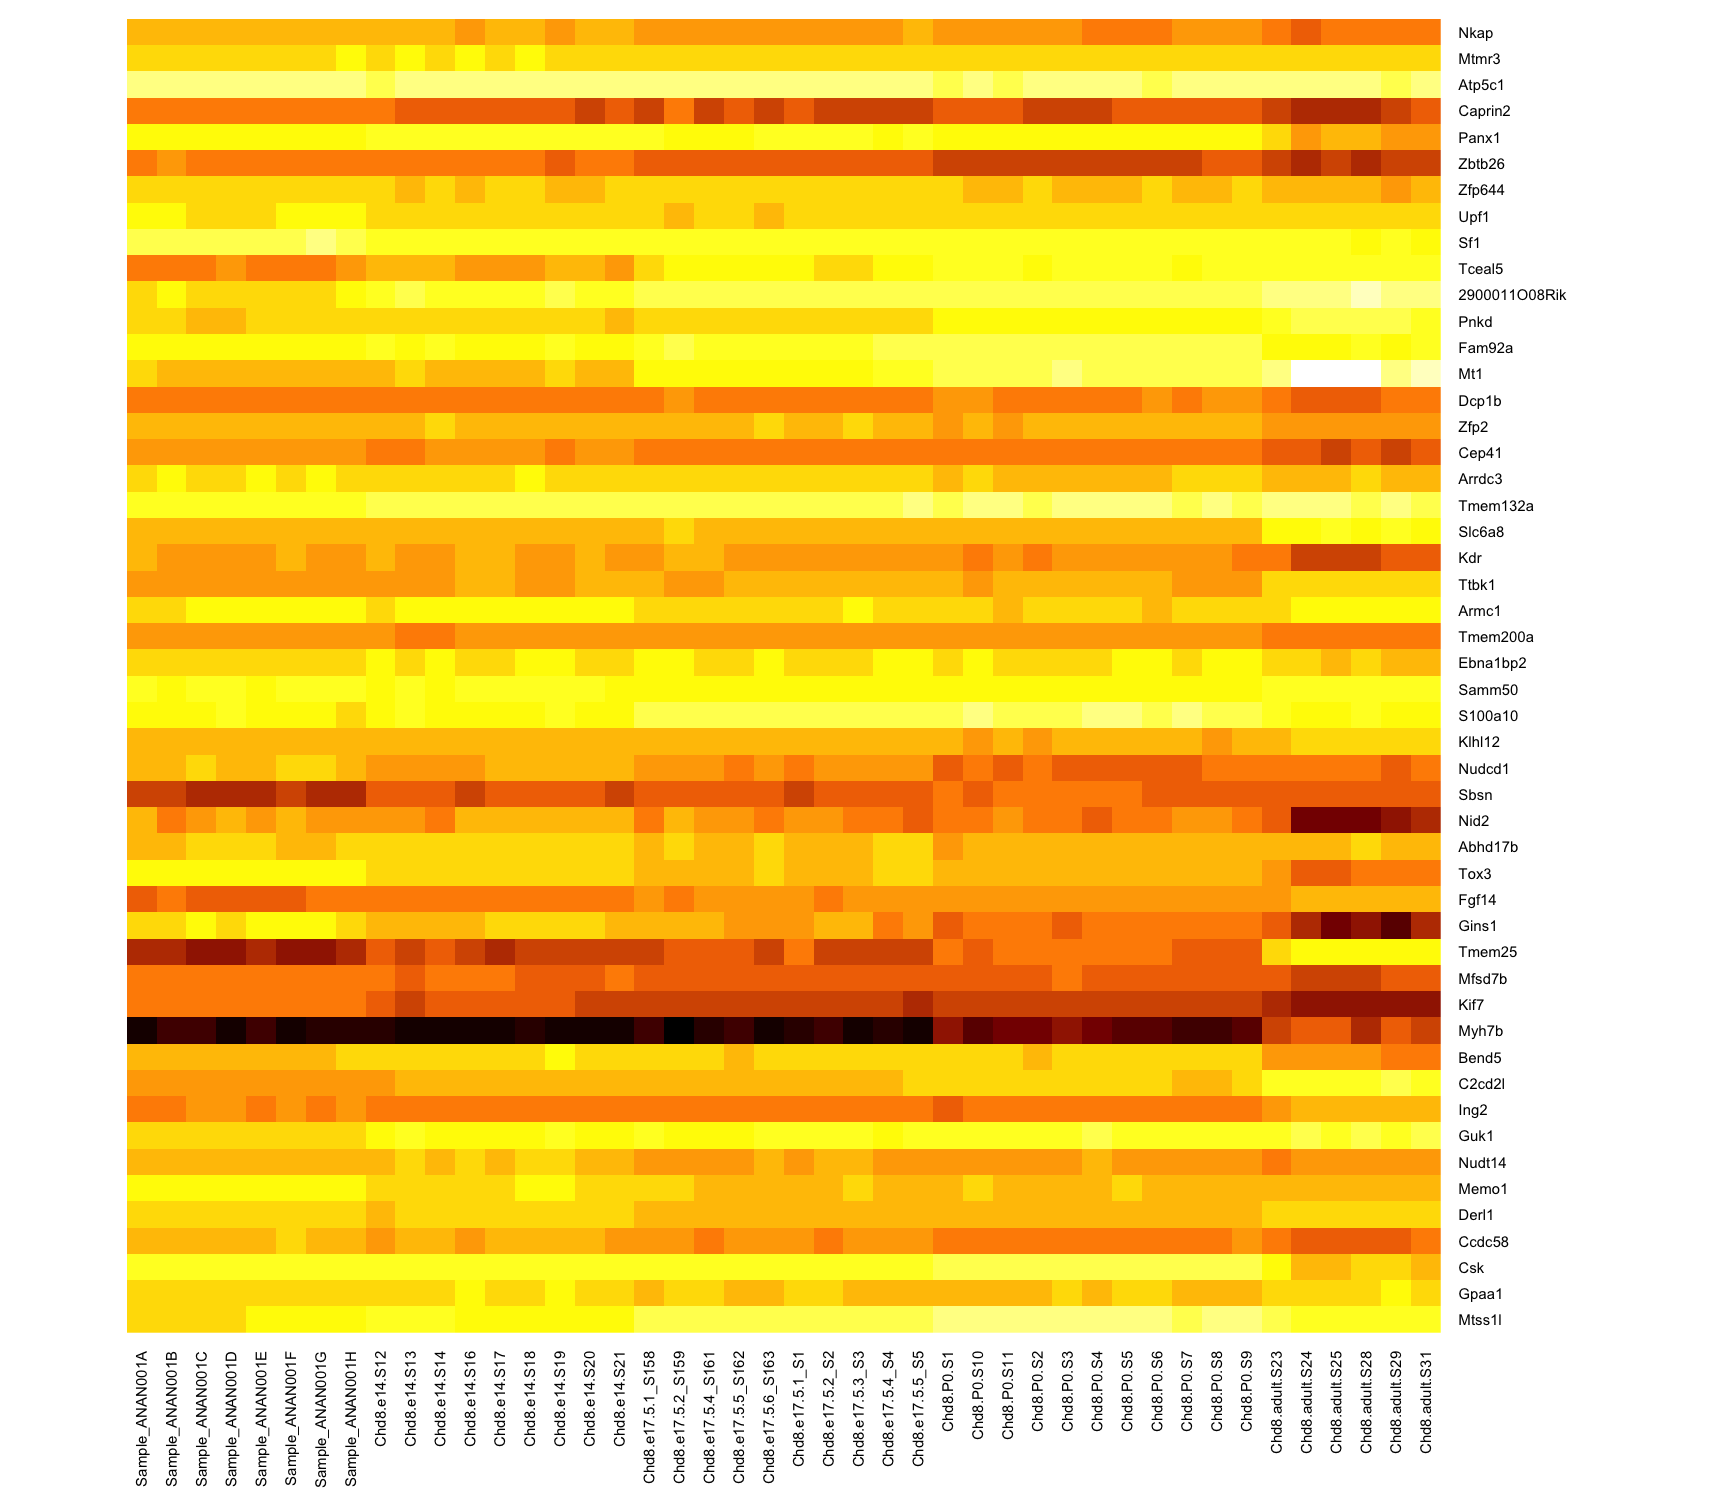
\includegraphics{Fig/unsupervised/unnamed-chunk-25-1} \end{center}


}

\normalsize
\end{column}

\begin{column}{.45\textwidth}
\scriptsize

\onslide<2>{


\begin{center}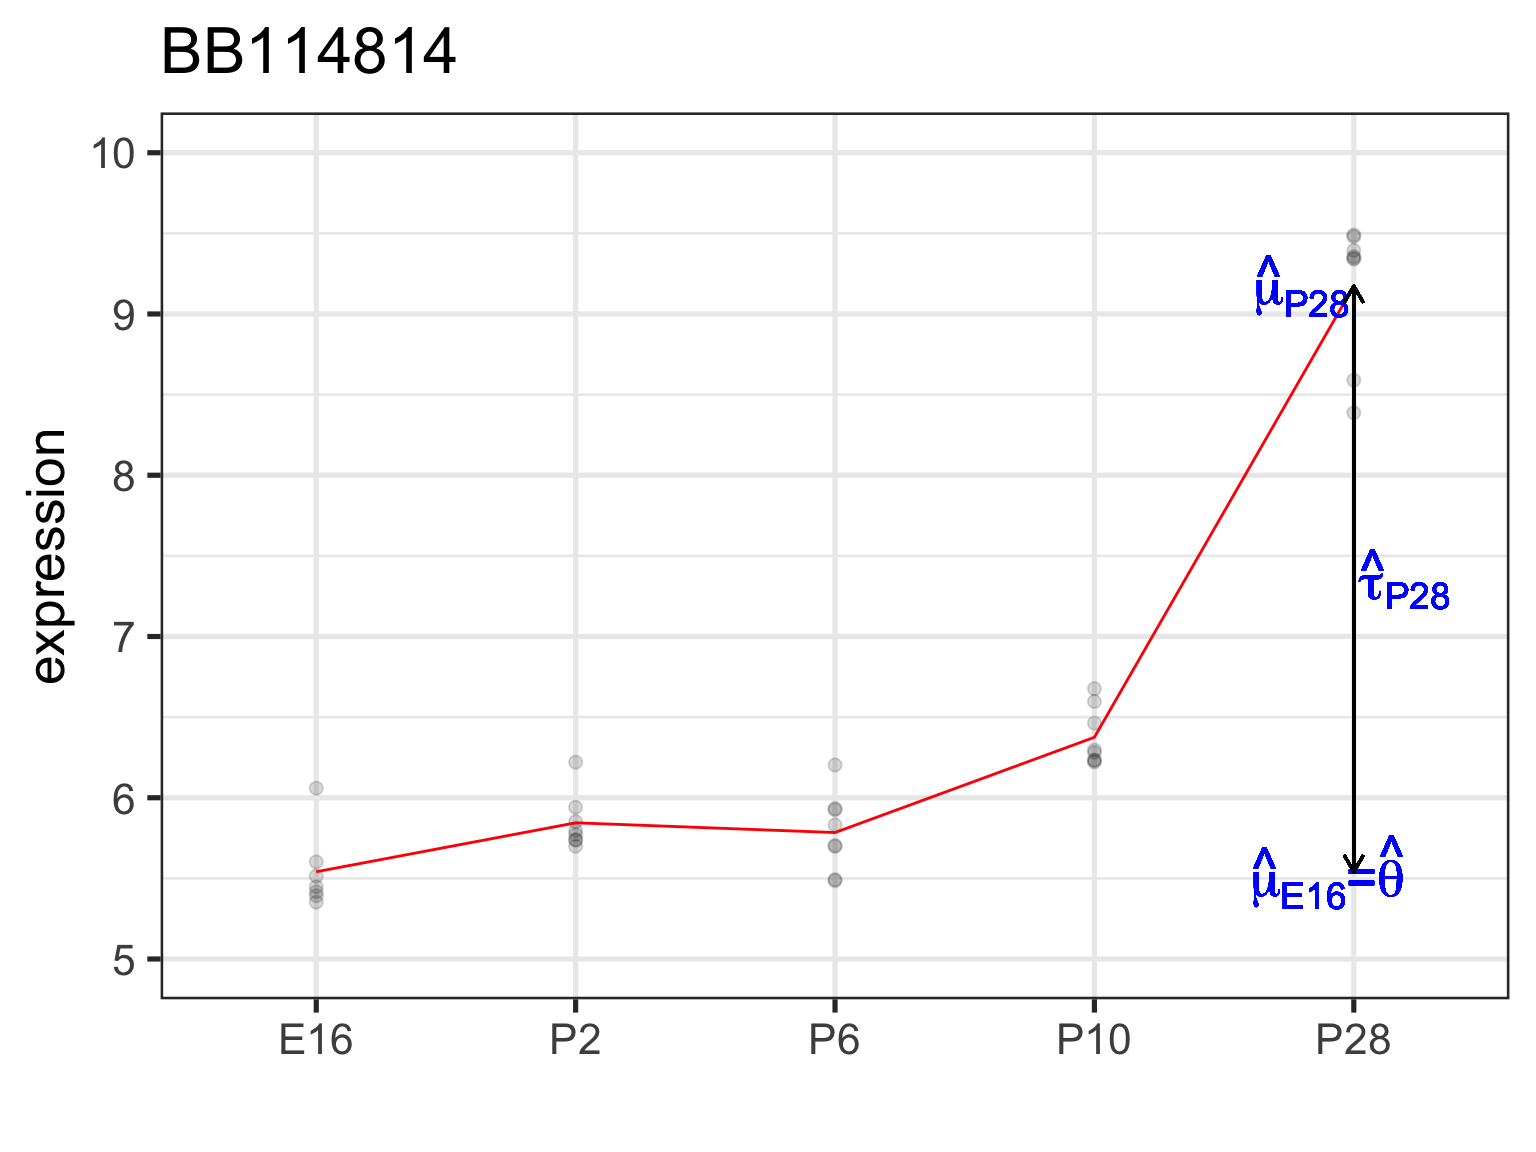
\includegraphics{Fig/unsupervised/unnamed-chunk-26-1} \end{center}


}

\normalsize
\end{column}
\end{columns}
\end{frame}

\begin{frame}{PCA: How do we recover ``common'' patterns from data?}
\protect\hypertarget{pca-how-do-we-recover-common-patterns-from-data}{}
Principal Component Analysis

\begin{columns}[T]
\begin{column}{.45\textwidth}
\begin{block}{(Pearson 1901)}
\protect\hypertarget{pearson-1901}{}
\begin{itemize}
\item
  Projection {[}of the original data{]} that minimizes the projection
  cost between the original and projected
\item
  The cost = mean squared distance
\end{itemize}
\end{block}
\end{column}

\begin{column}{.45\textwidth}
\begin{block}{(Hotelling 1933)}
\protect\hypertarget{hotelling-1933}{}
\begin{itemize}
\item
  Orthogonal projection of data into a lower-dimensional
  \textbf{{[}principal{]}} sub-space,
\item
  such that the total \textbf{variation of the projected} is maximized
\end{itemize}
\end{block}
\end{column}
\end{columns}
\end{frame}

\begin{frame}{What do we mean by projection to a low-dimensional space?}
\protect\hypertarget{what-do-we-mean-by-projection-to-a-low-dimensional-space}{}
\scriptsize

\normalsize

\textbf{Recap:} We learned that a multivariate linear regression
projects a data vector \(\mathbf{y}\) onto the column space of the
design matrix \(U\):

\[\left(\begin{array}{l}
X_{1}\\
X_{2}\\
\vdots \\
X_{m}\\
\end{array}
\right) = 
\left(
\begin{array}{l l l}
U_{11} & \ldots & U_{1k}\\
U_{21} & \ldots & U_{2k}\\
\vdots & \vdots & \vdots \\
U_{m1} & \ldots & U_{mk}\\
\end{array} 
\right)
\left(
\begin{array}{l}
W_{1}\\
\vdots\\
W_{k}
\end{array}
\right)
+ 
\left(
\begin{array}{l}
\epsilon_{1}\\
\epsilon_{2}\\
\vdots\\
\epsilon_{m}
\end{array}
\right)\]

or

\(\mathbf{x} = U \mathbf{w} + \epsilon\), for many columns,
\(X = U W + E\).

\begin{itemize}
\item
  If we \textbf{knew} \(U\), we would be able to solve weights \(W\). If
  \(k = 2\), it would result in a projection to the 2D space.
\item
  Unlike regression, we need ask: How do we know this unknown \(U\)
  matrix?
\end{itemize}
\end{frame}

\begin{frame}{What is a projection matrix?}
\protect\hypertarget{what-is-a-projection-matrix}{}
The purpose of a multivariate regression-based prediction:

\[\mathbf{x} \to \hat{\mathbf{x}} = U \mathbf{w}\]

The least-square solution for the \(W\):

\[\hat{\mathbf{w}} = (U^{\top}U)^{-1} U^{\top}\mathbf{x}\]

Then we have

\[\hat{\mathbf{x}} = \underbrace{U (U^{\top}U)^{-1} U^{\top}}_{\textsf{\color{red} projection matrix}} \mathbf{x}\]

You can think of ``projection'' as \textbf{``prediction'' in the linear
space} defined by the columns of a design matrix.
\end{frame}

\begin{frame}{What will be a good ``feature'' (the \(U\) matrix) to
regress on?}
\protect\hypertarget{what-will-be-a-good-feature-the-u-matrix-to-regress-on}{}
\begin{columns}[T]
\begin{column}{.35\textwidth}
\scriptsize

\only<1>{


\begin{center}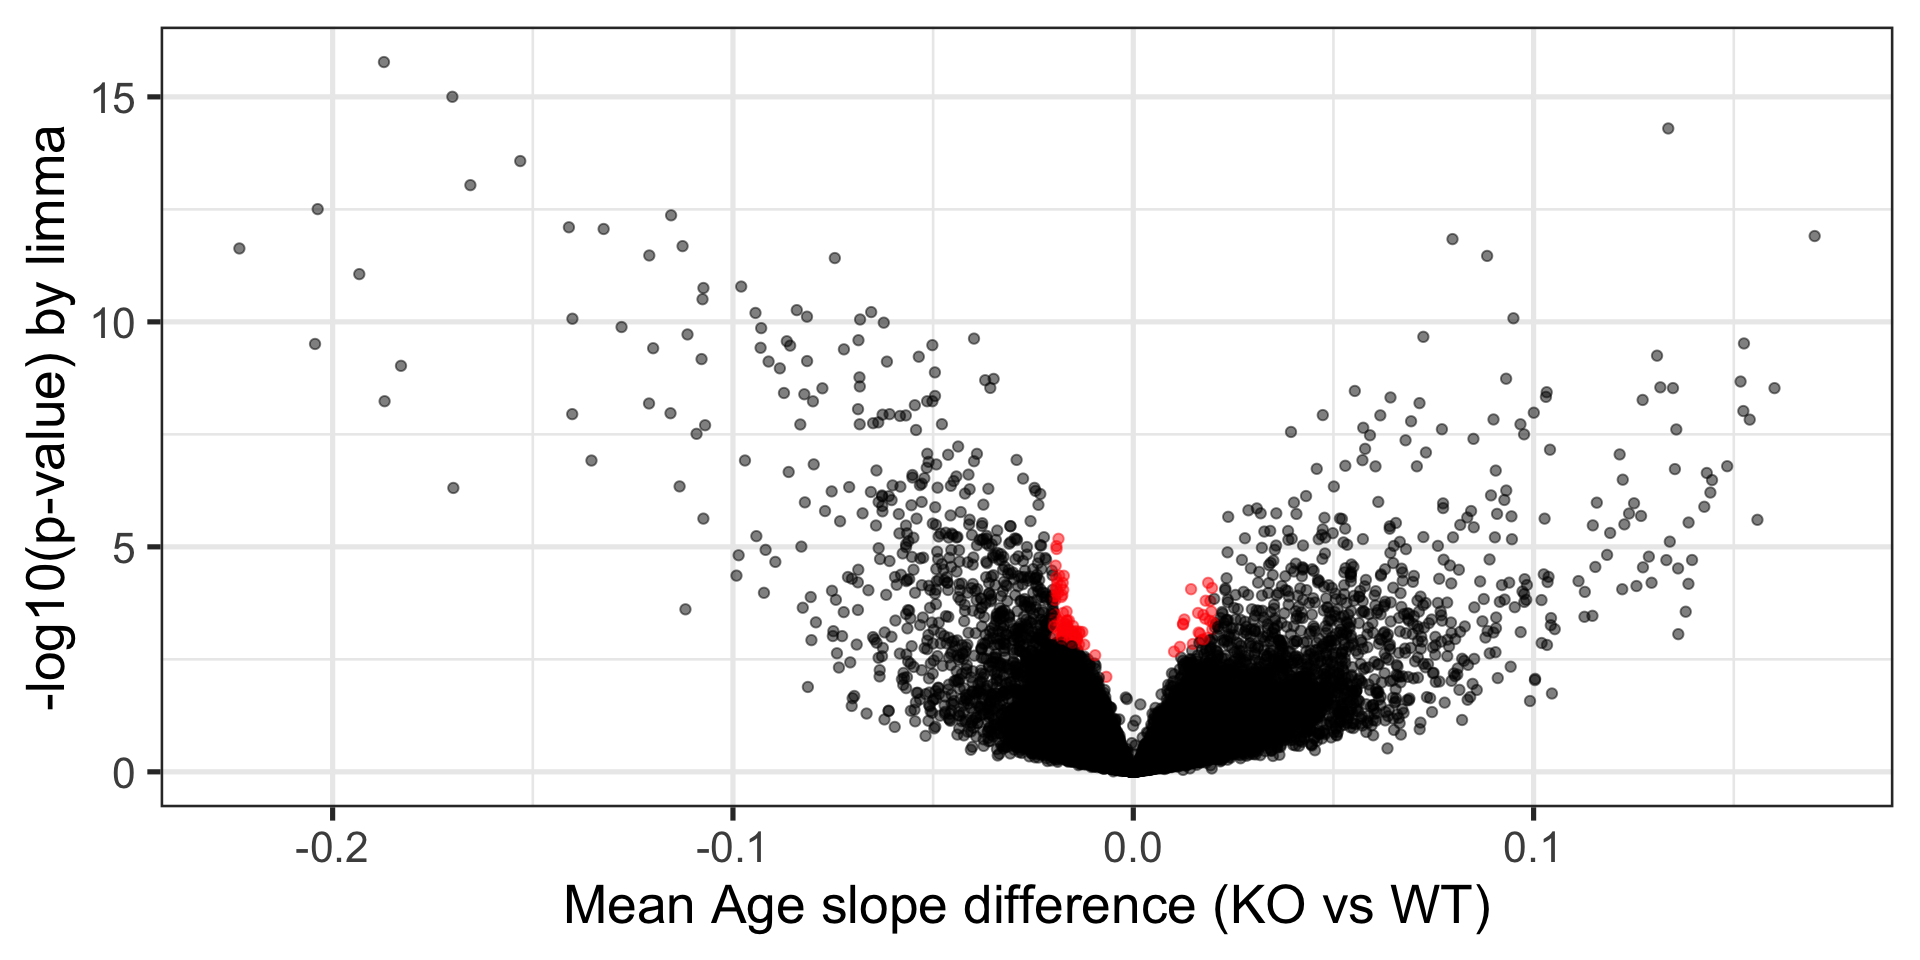
\includegraphics{Fig/unsupervised/unnamed-chunk-28-1} \end{center}


}

\normalsize

\scriptsize

\normalsize

\scriptsize

\only<2>{


\begin{center}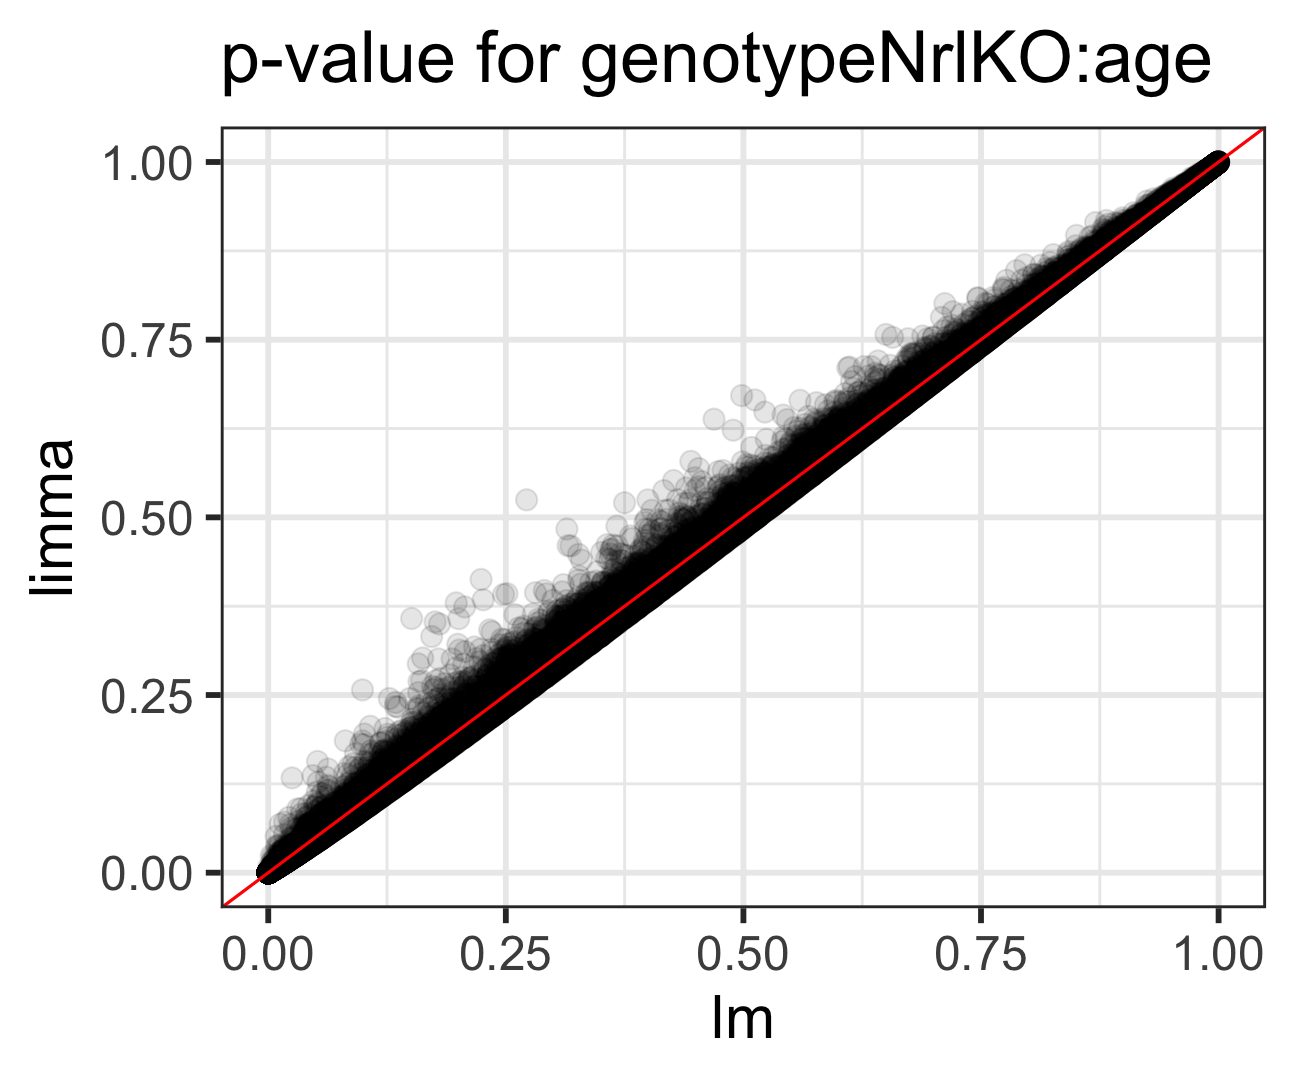
\includegraphics{Fig/unsupervised/unnamed-chunk-30-1} \end{center}


}

\normalsize

\scriptsize

\only<3>{


\begin{center}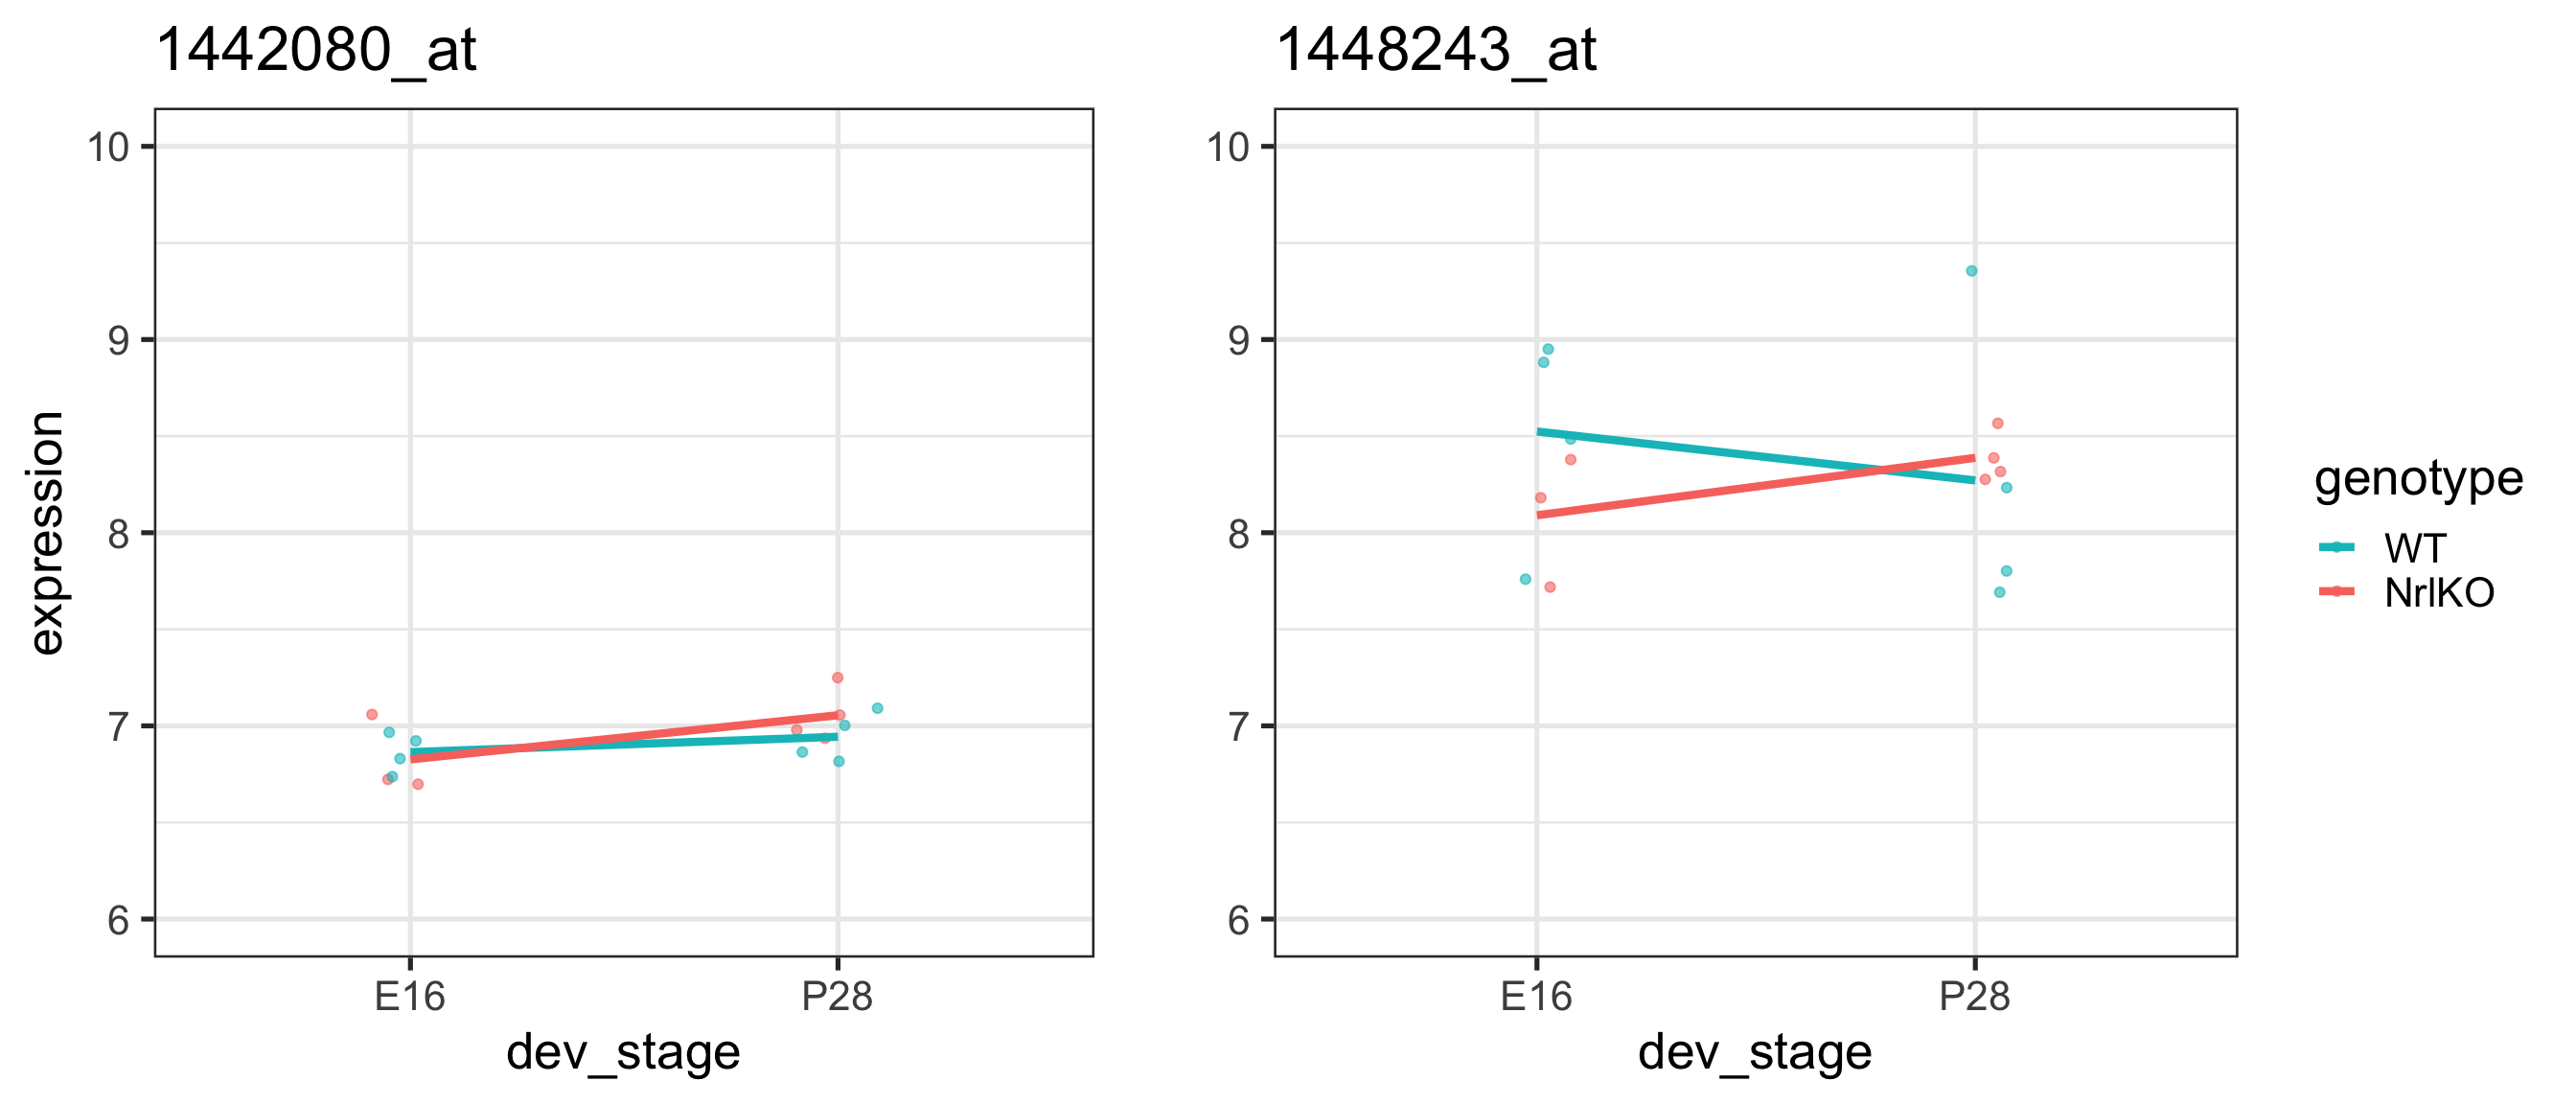
\includegraphics{Fig/unsupervised/unnamed-chunk-31-1} \end{center}


}

\normalsize
\end{column}

\begin{column}{.65\textwidth}
\scriptsize

\only<2>{


\begin{center}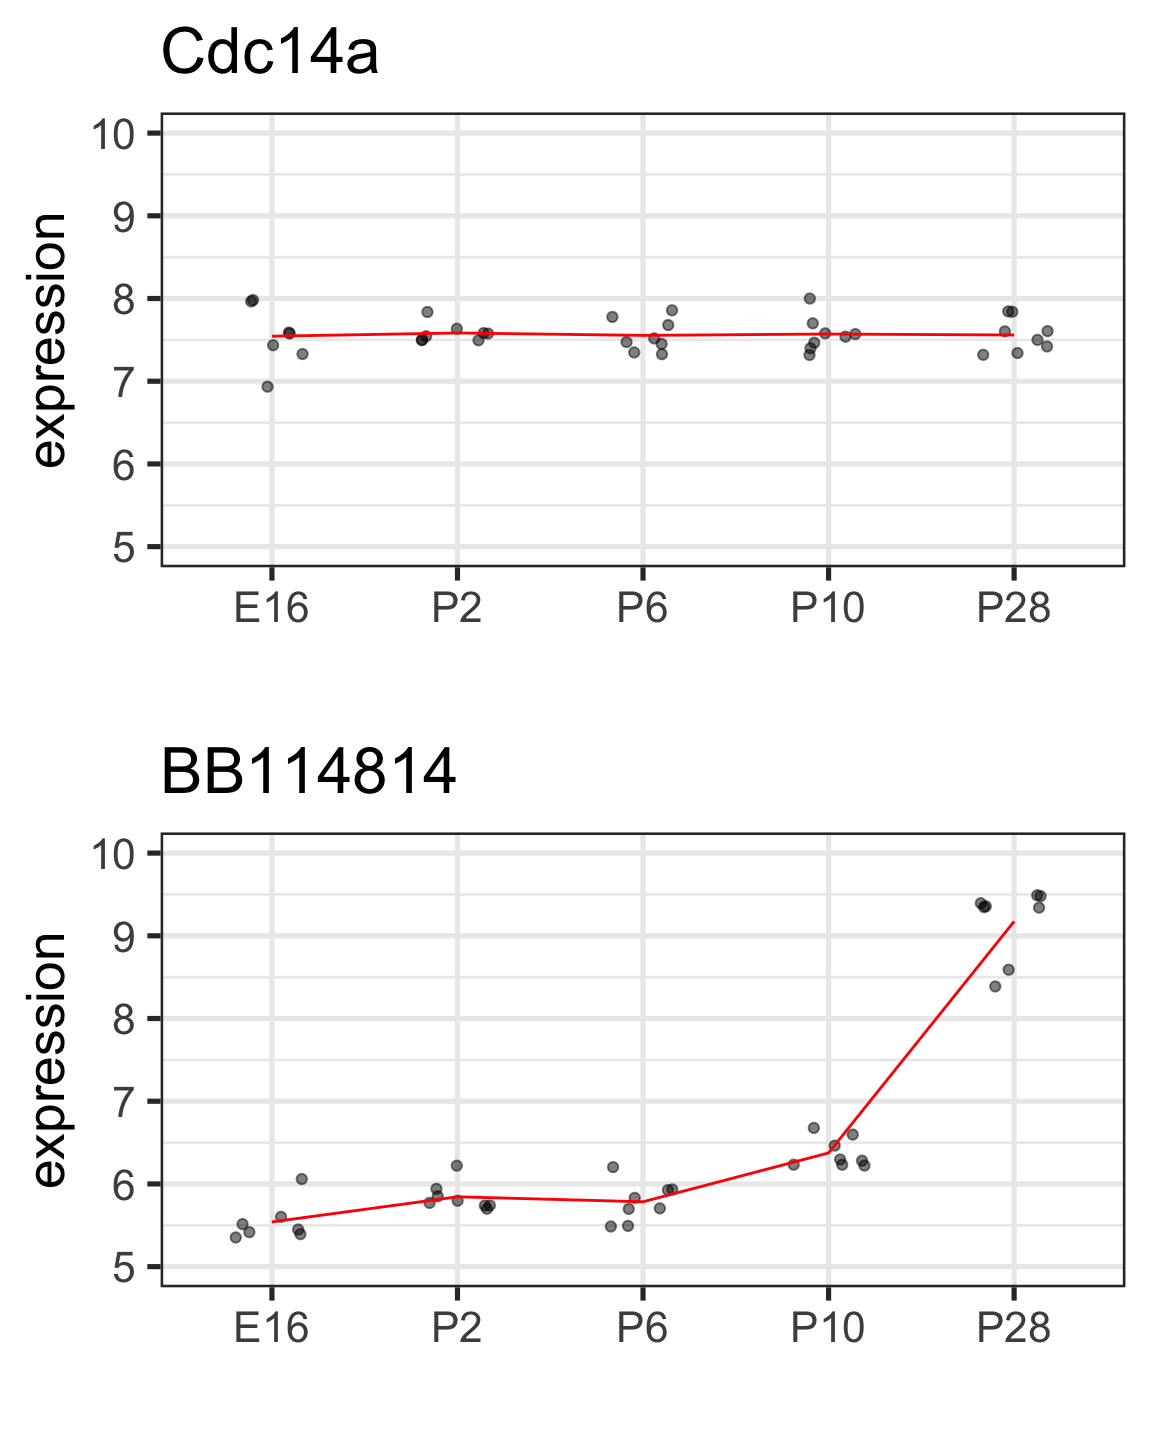
\includegraphics{Fig/unsupervised/unnamed-chunk-32-1} \end{center}


}

\normalsize

\scriptsize

\only<3>{


\begin{center}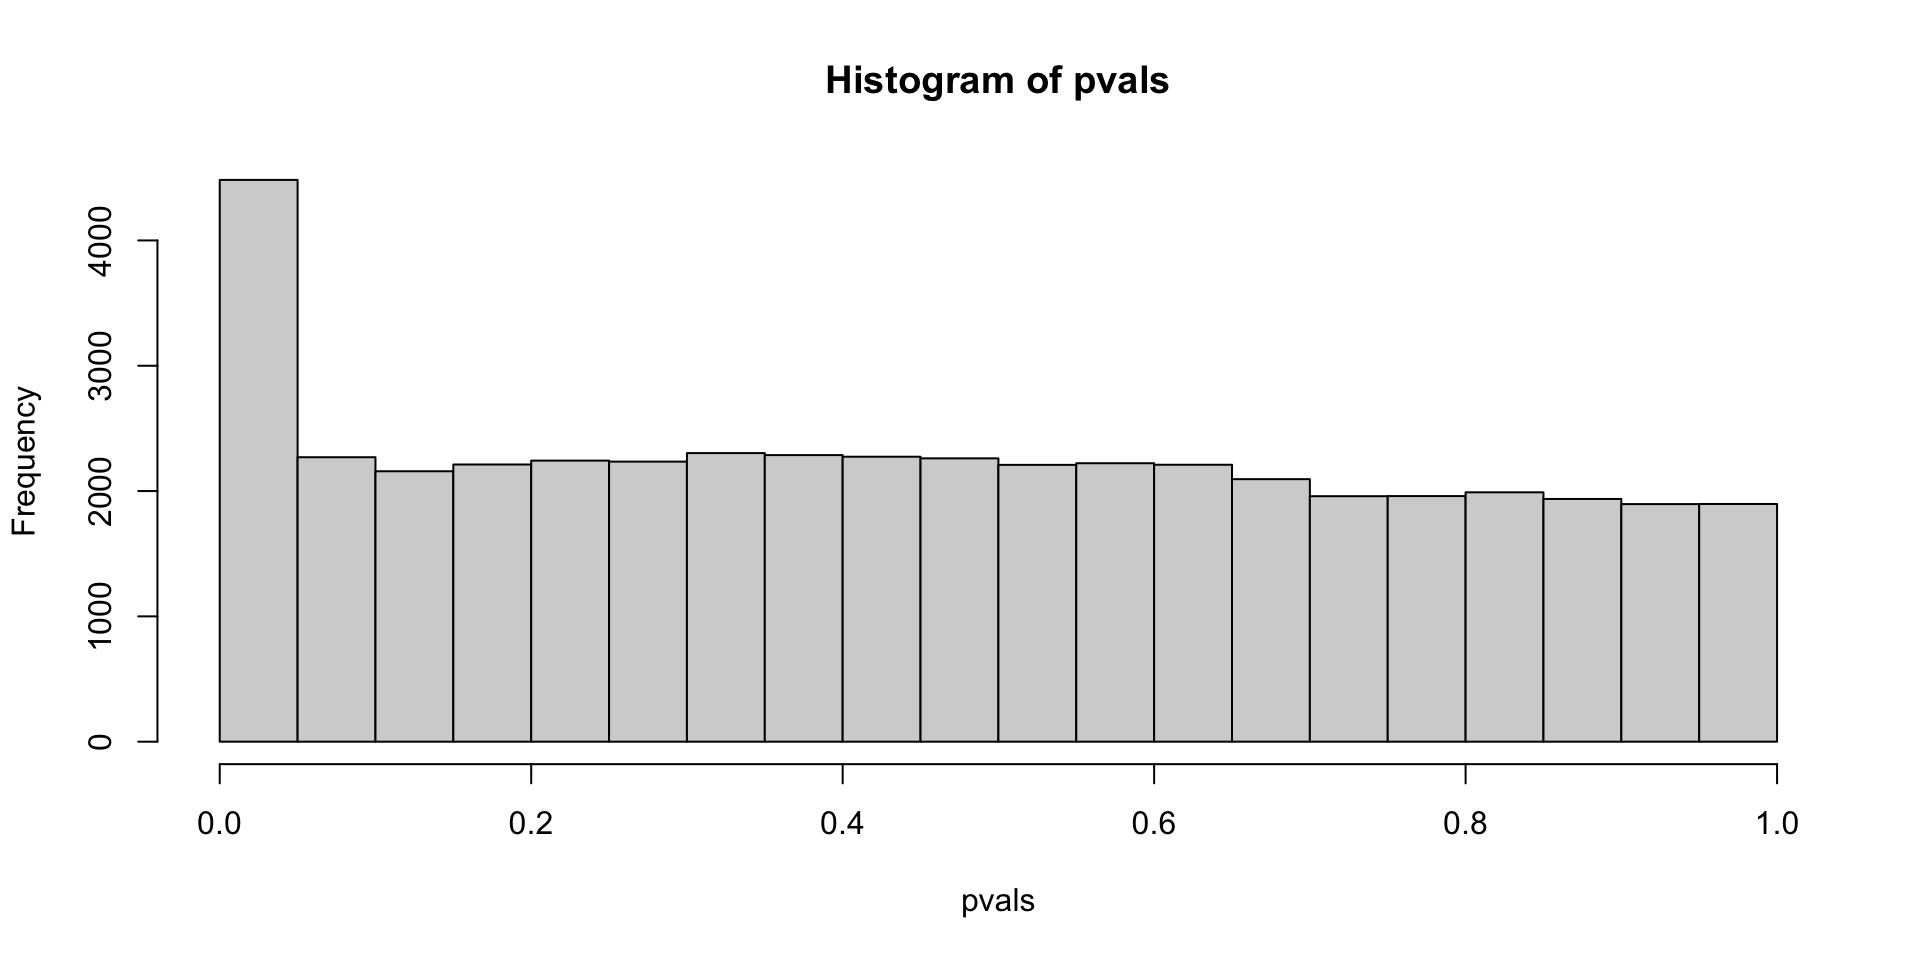
\includegraphics{Fig/unsupervised/unnamed-chunk-33-1} \end{center}


}

\normalsize
\end{column}
\end{columns}
\end{frame}

\begin{frame}{How about an average vector?}
\protect\hypertarget{how-about-an-average-vector}{}
\begin{columns}[T]
\begin{column}{.35\textwidth}
\scriptsize

\only<1>{


\begin{center}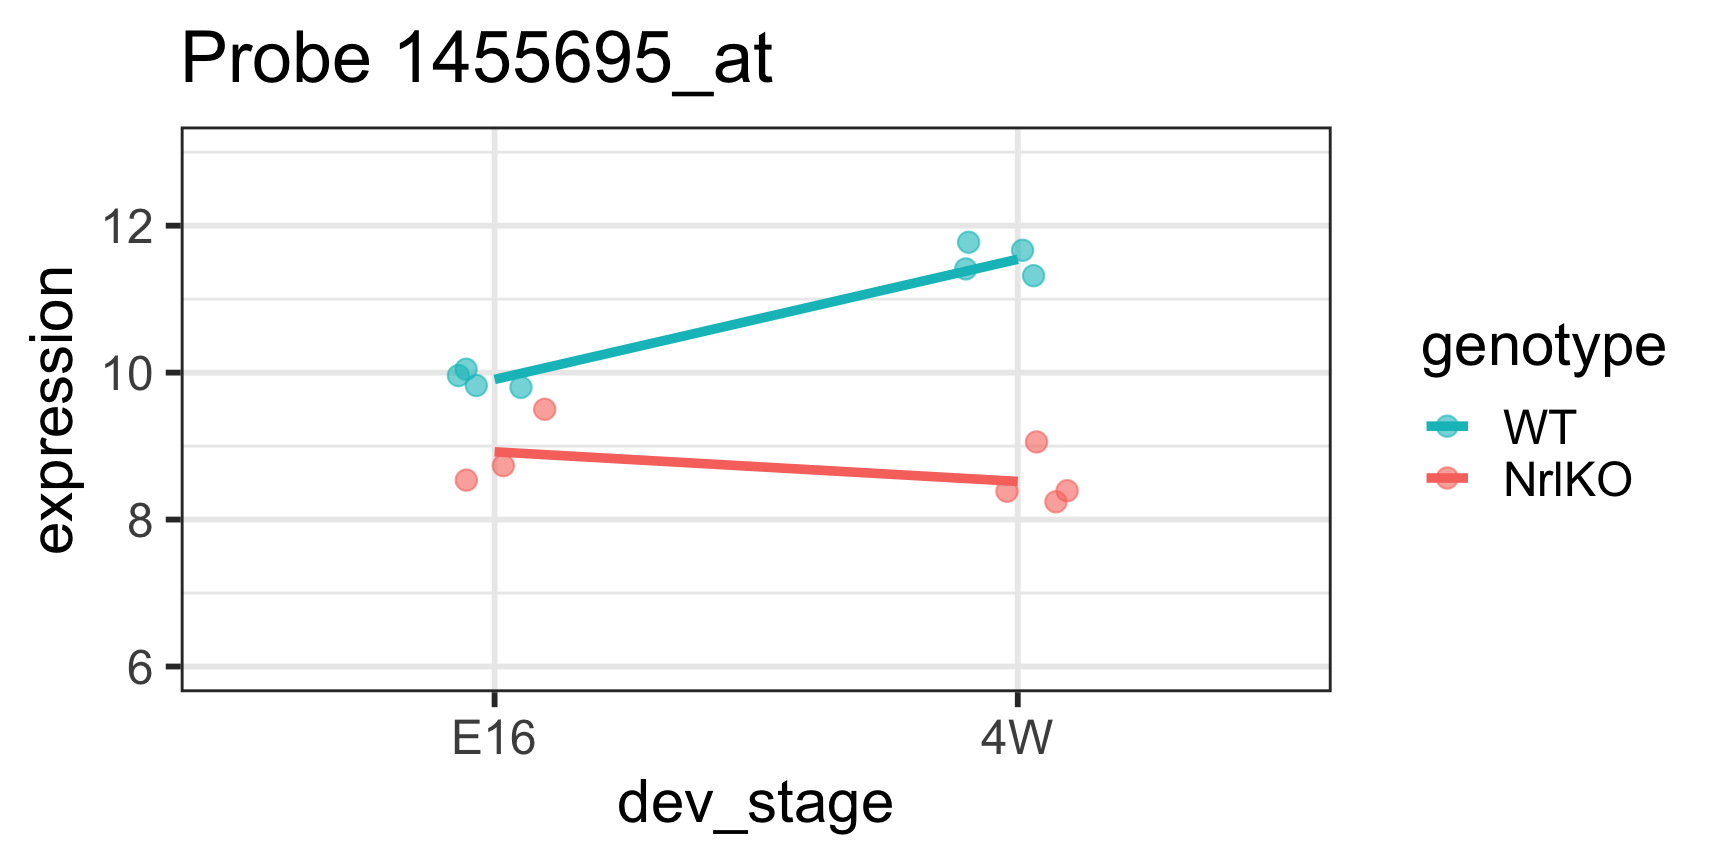
\includegraphics{Fig/unsupervised/unnamed-chunk-34-1} \end{center}


}

\normalsize

\scriptsize

\normalsize

\scriptsize

\only<2>{


\begin{center}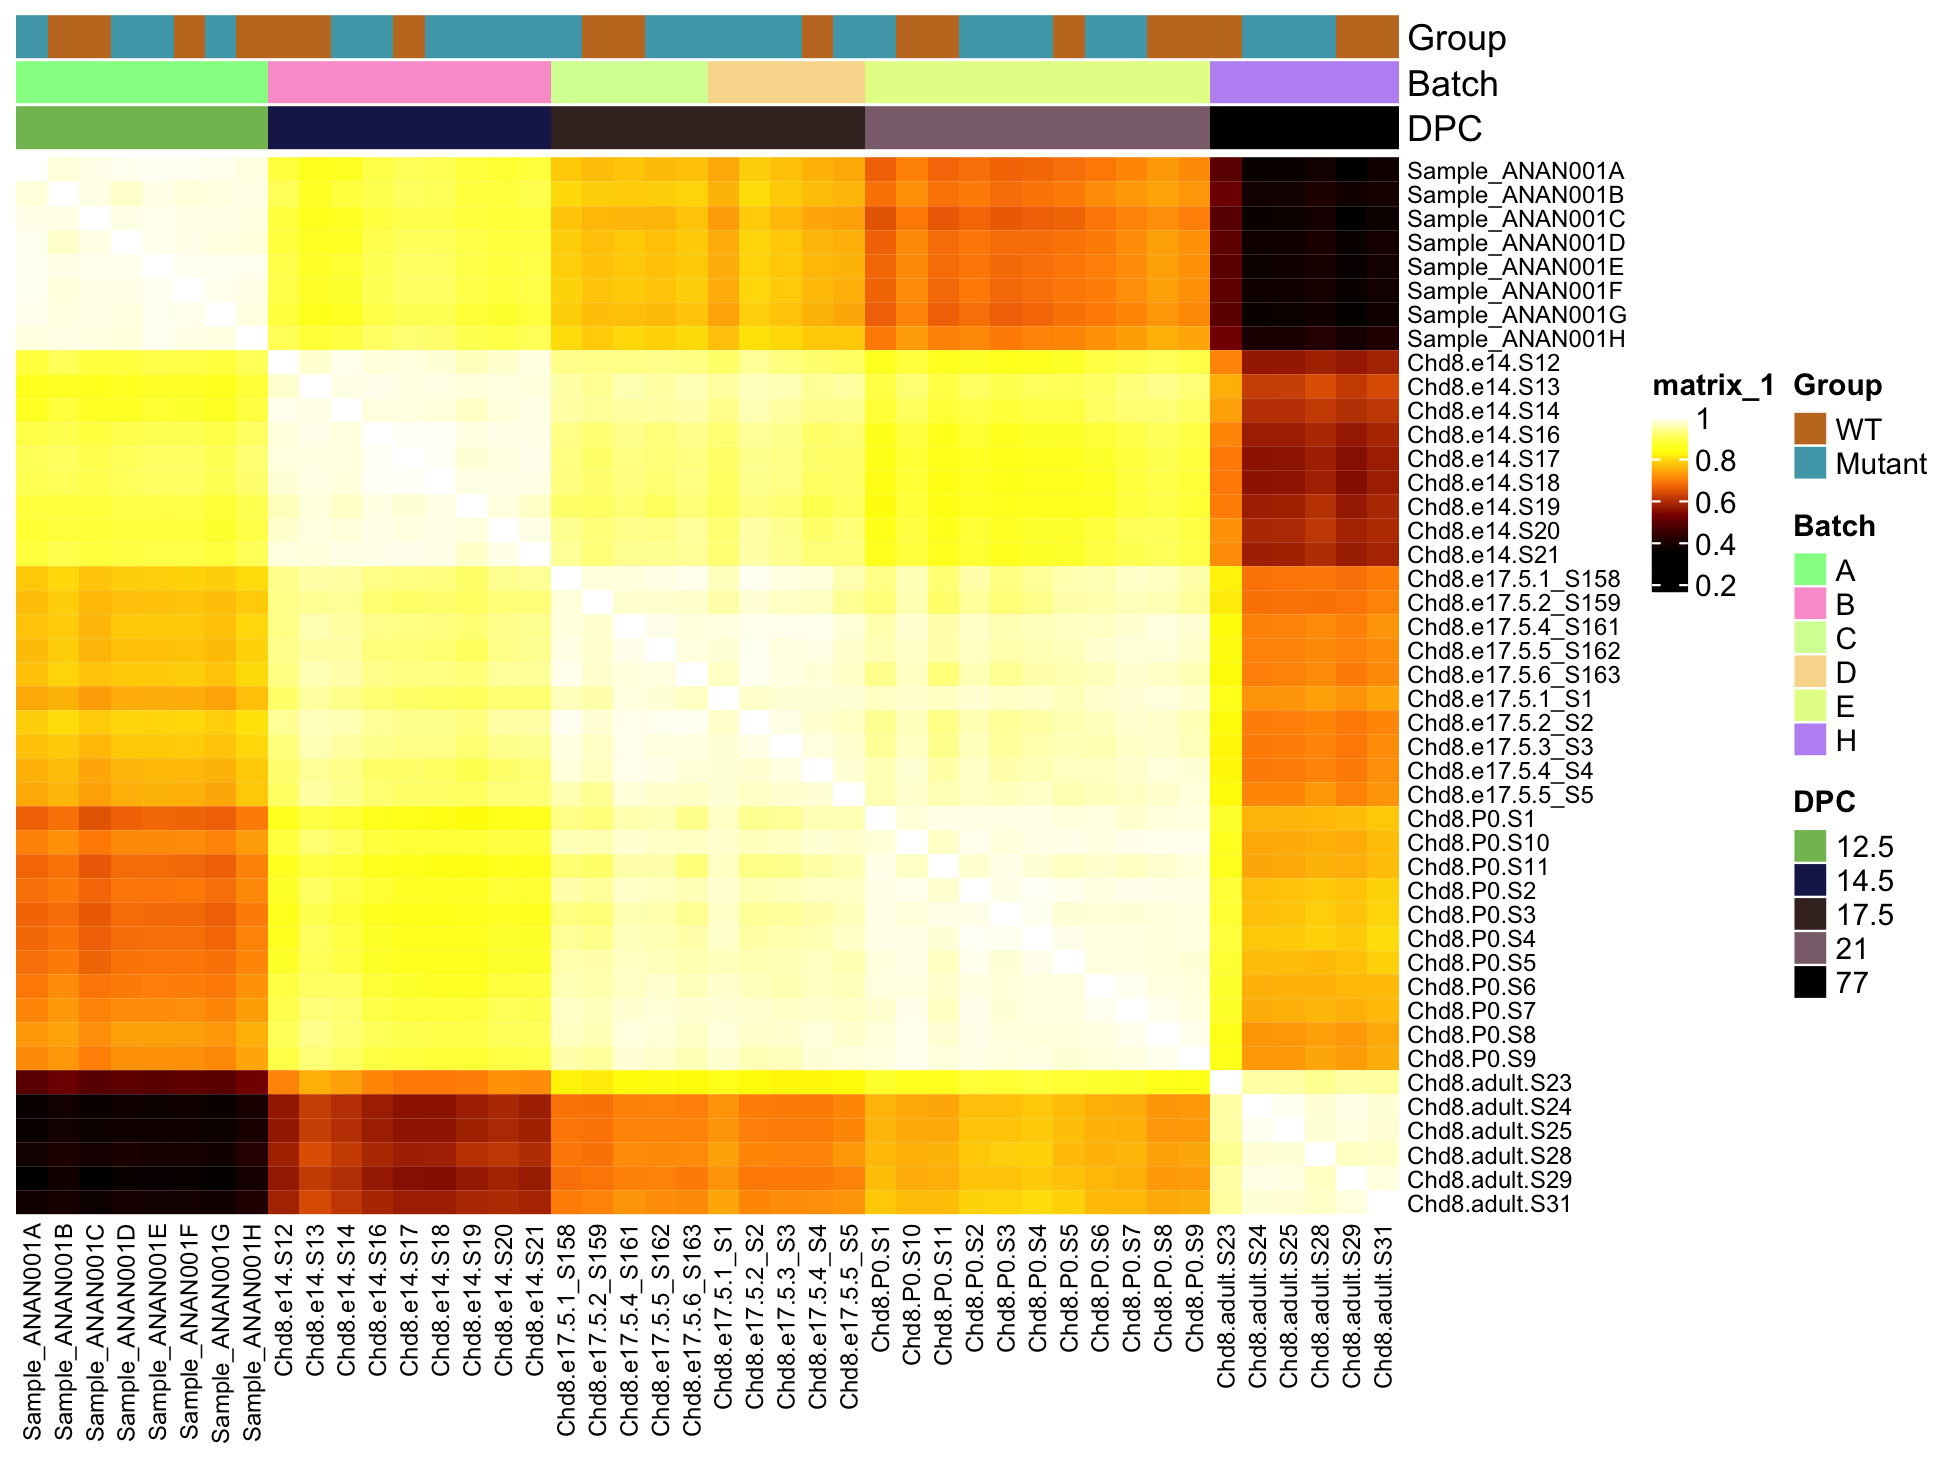
\includegraphics{Fig/unsupervised/unnamed-chunk-36-1} \end{center}


}

\normalsize

\scriptsize

\only<3>{


\begin{center}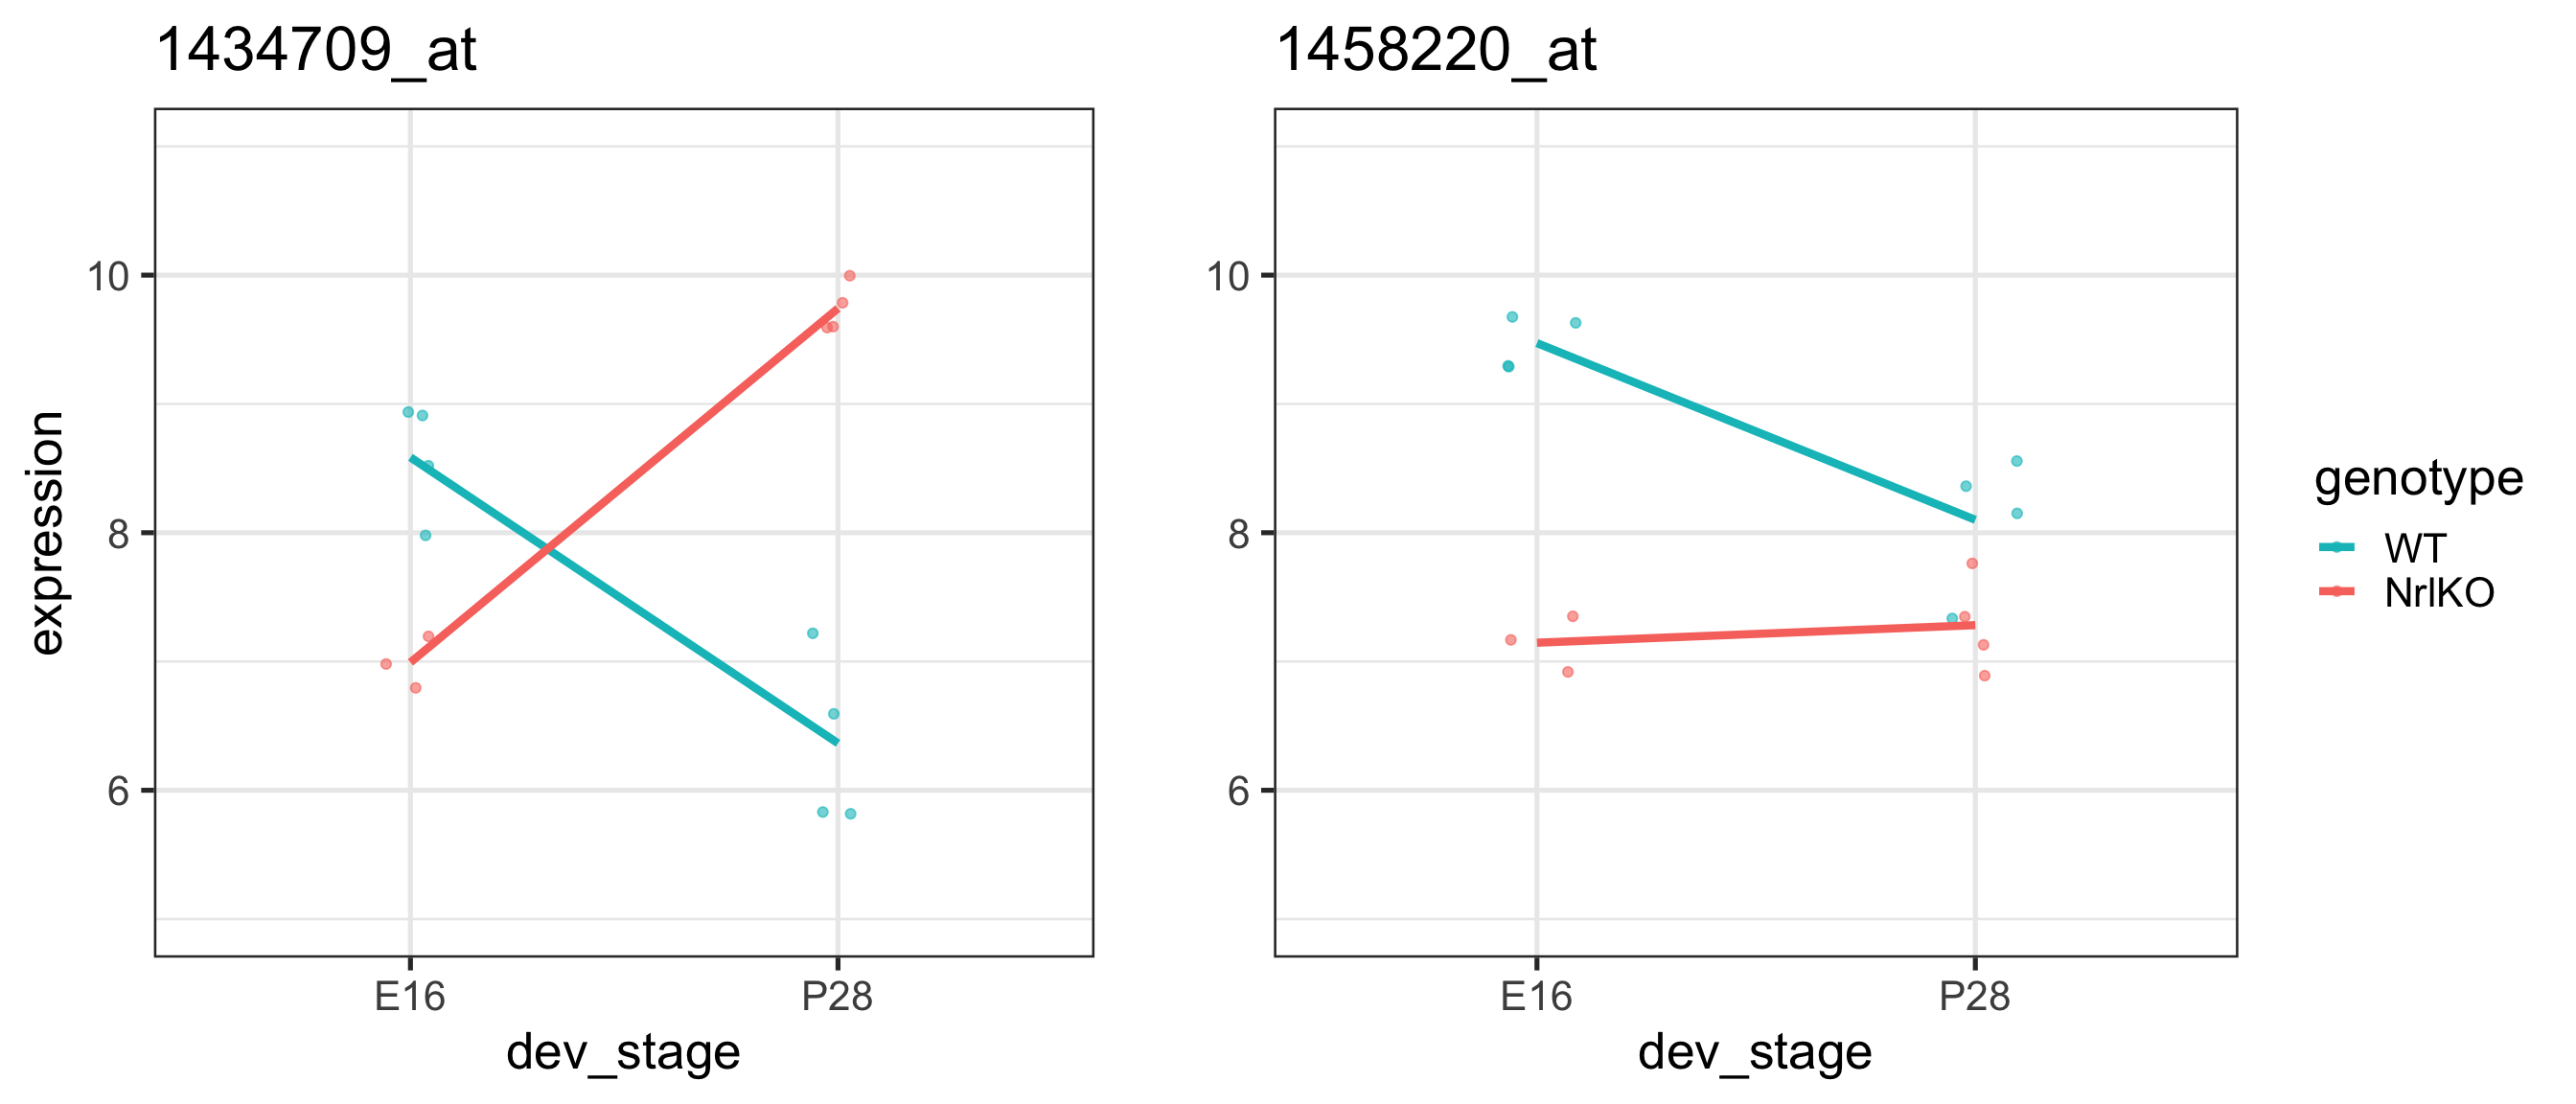
\includegraphics{Fig/unsupervised/unnamed-chunk-37-1} \end{center}


}

\normalsize
\end{column}

\begin{column}{.65\textwidth}
\scriptsize

\only<2>{


\begin{center}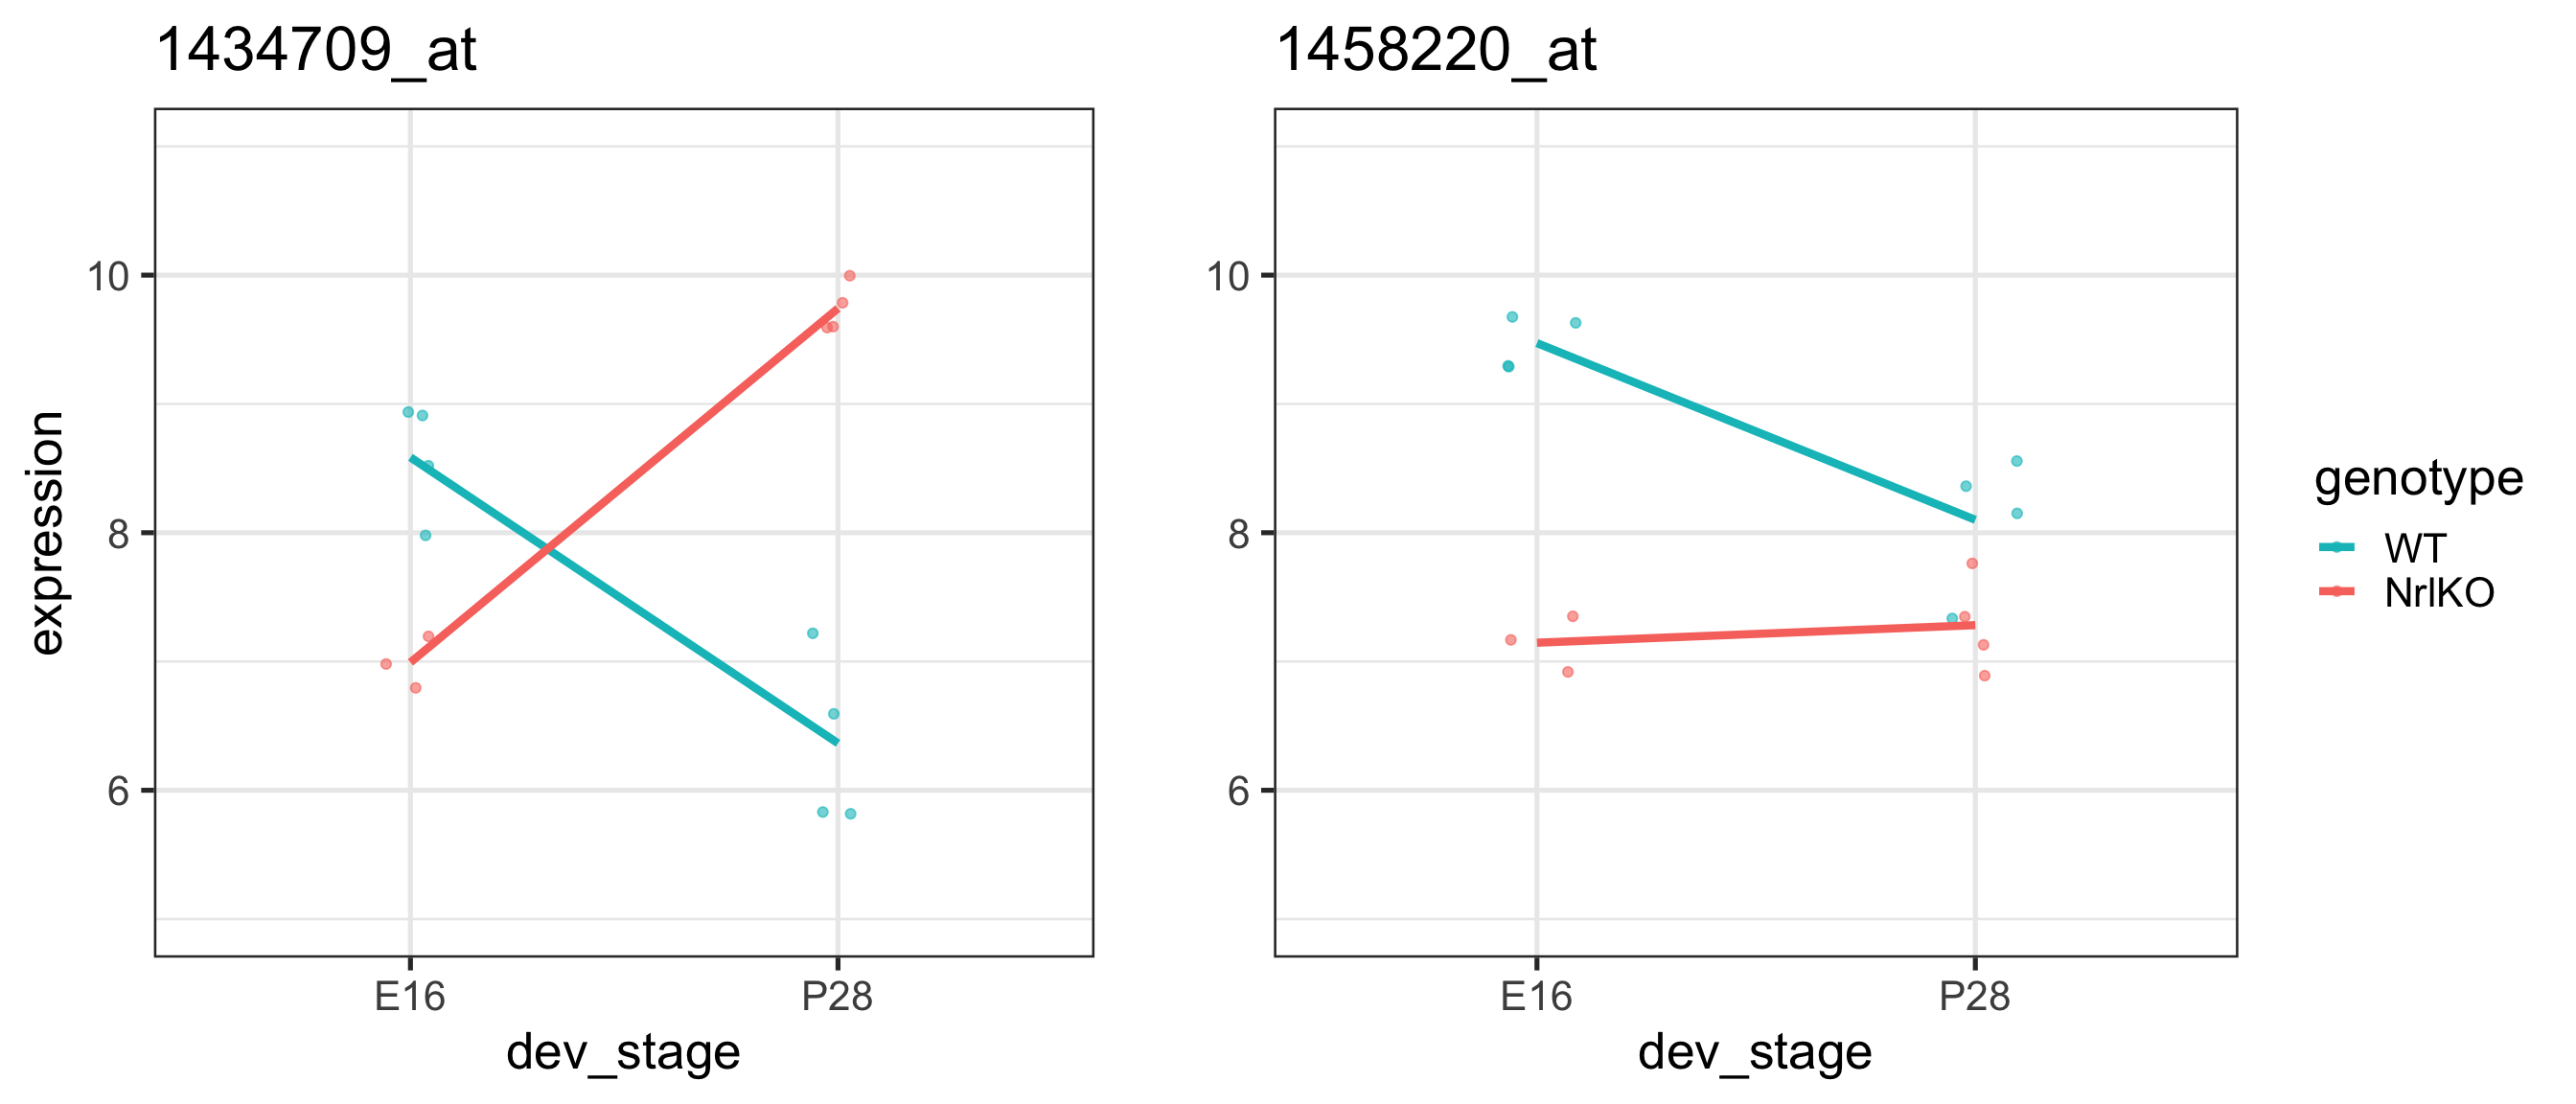
\includegraphics{Fig/unsupervised/unnamed-chunk-38-1} \end{center}


}

\normalsize

\scriptsize

\only<3>{


\begin{center}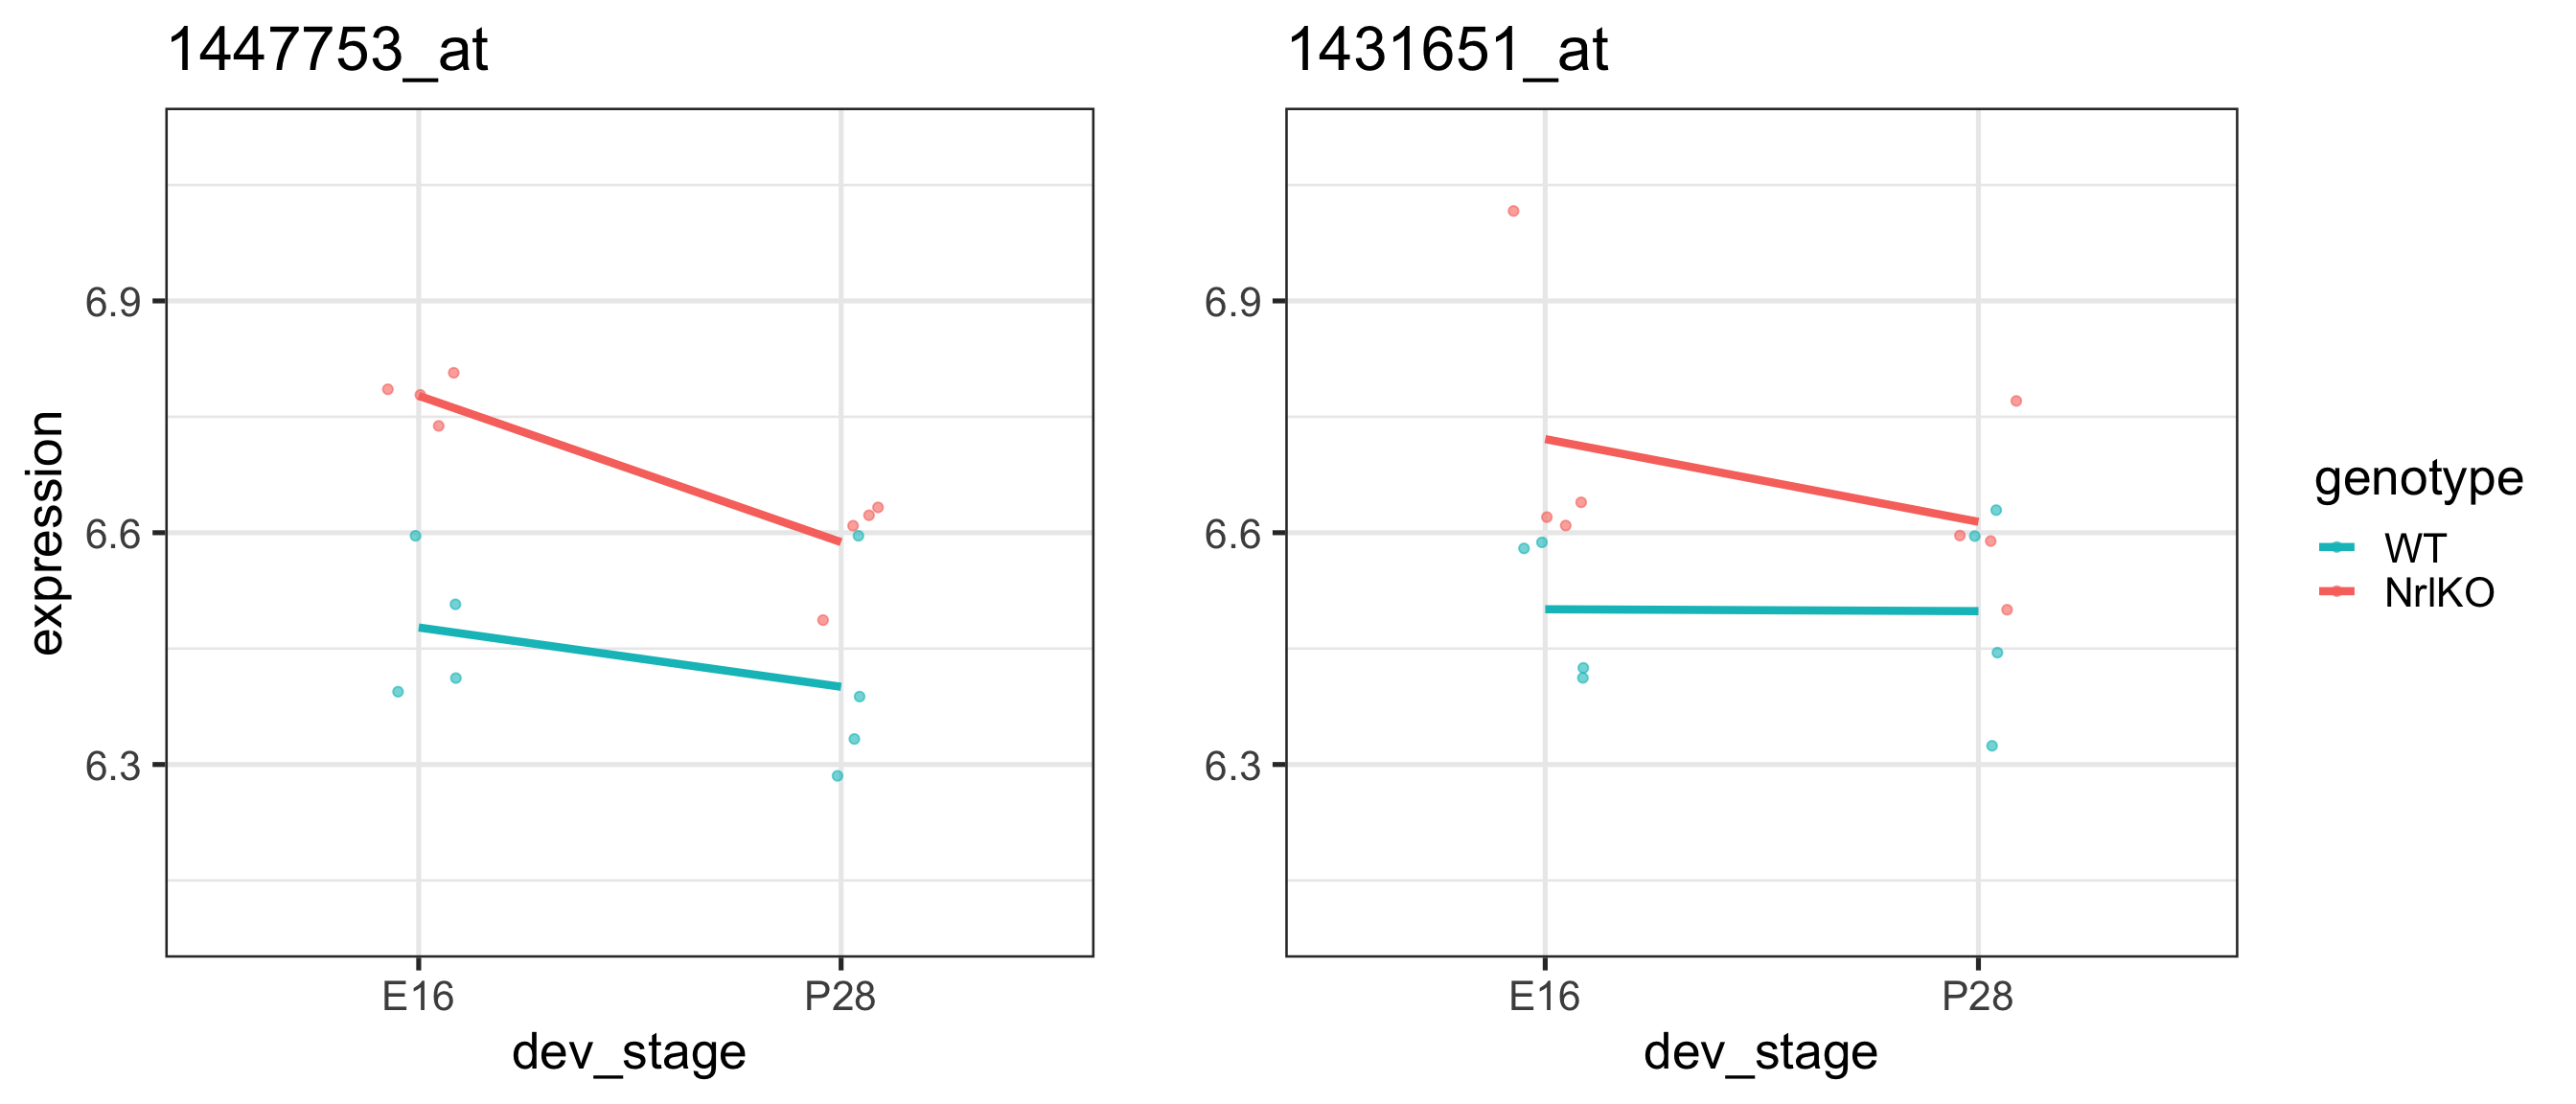
\includegraphics{Fig/unsupervised/unnamed-chunk-39-1} \end{center}


}

\normalsize
\end{column}
\end{columns}
\end{frame}

\begin{frame}{Let's try out random projection}
\protect\hypertarget{lets-try-out-random-projection}{}
\begin{columns}[T]
\begin{column}{.35\textwidth}
\scriptsize

\only<1>{


\begin{center}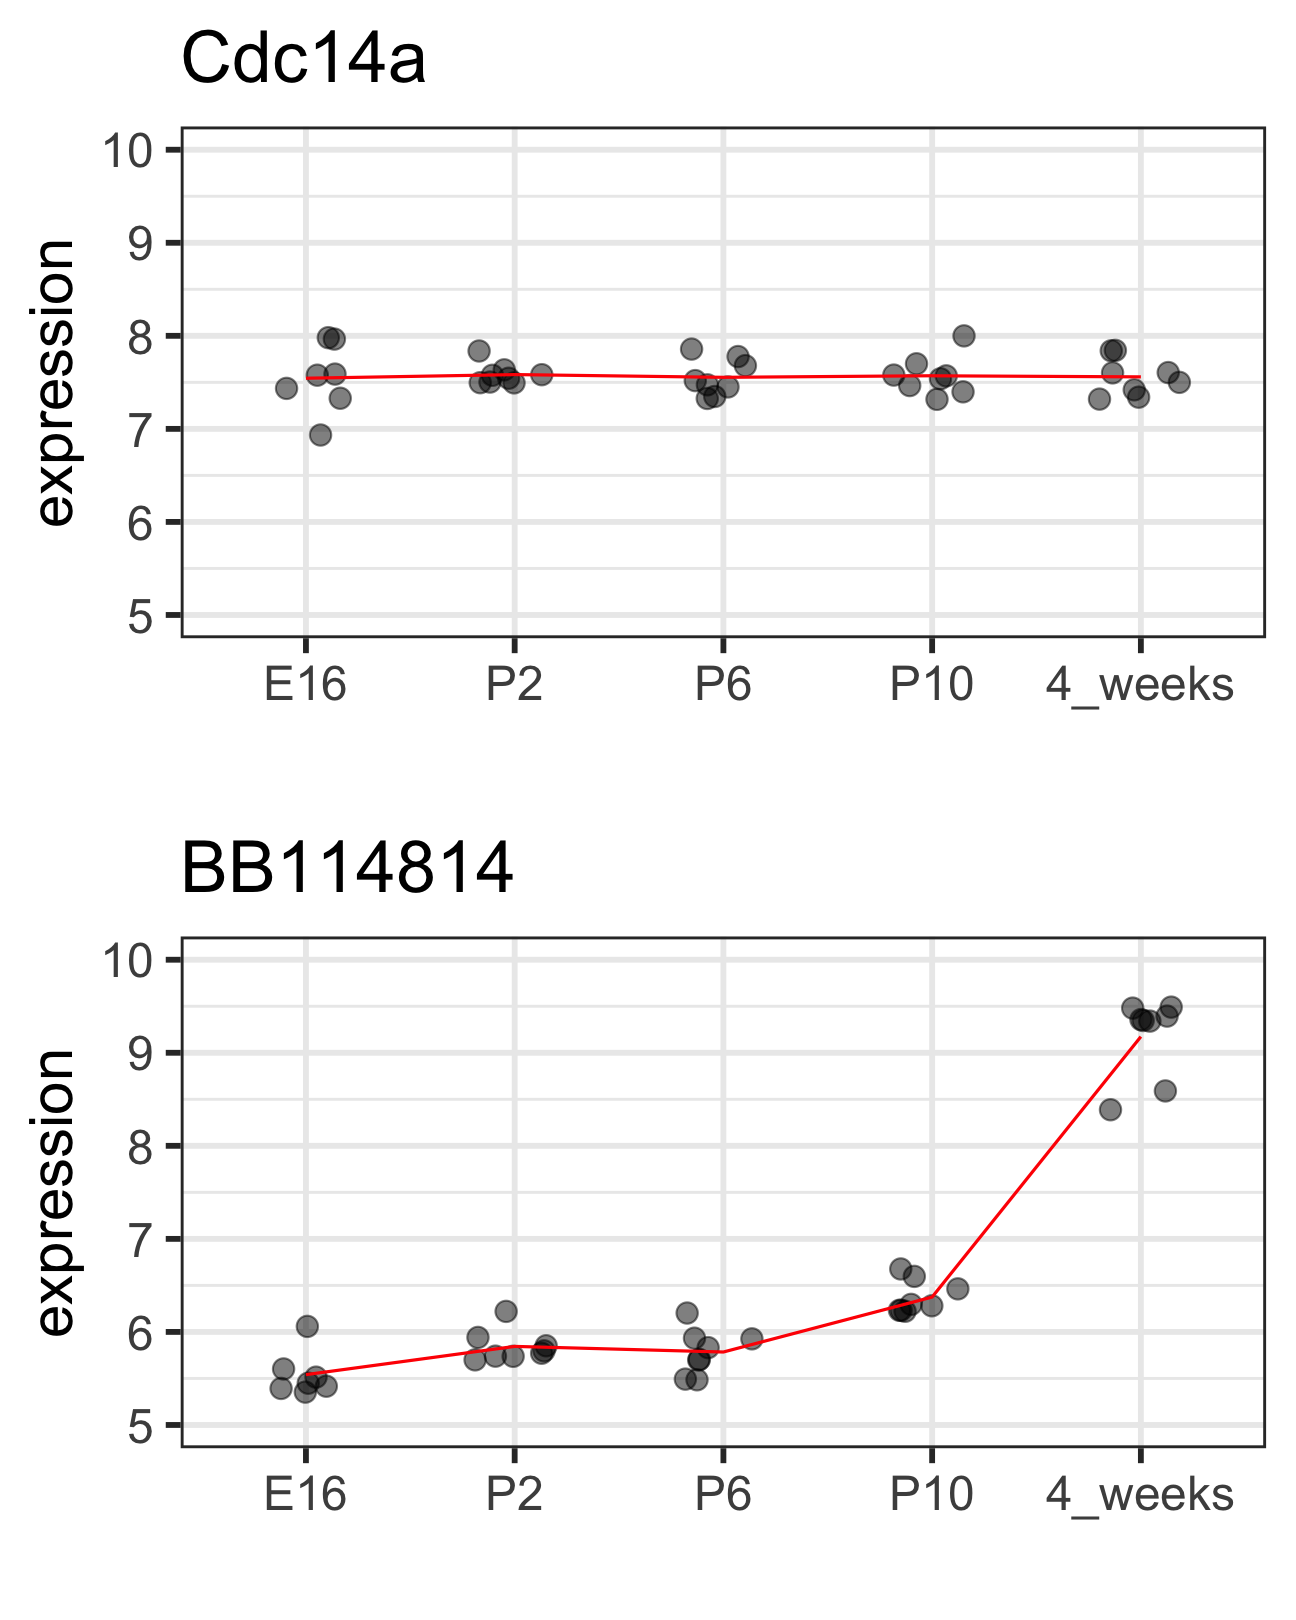
\includegraphics{Fig/unsupervised/unnamed-chunk-40-1} \end{center}


}

\normalsize

\scriptsize

\normalsize

\scriptsize

\only<2>{


\begin{center}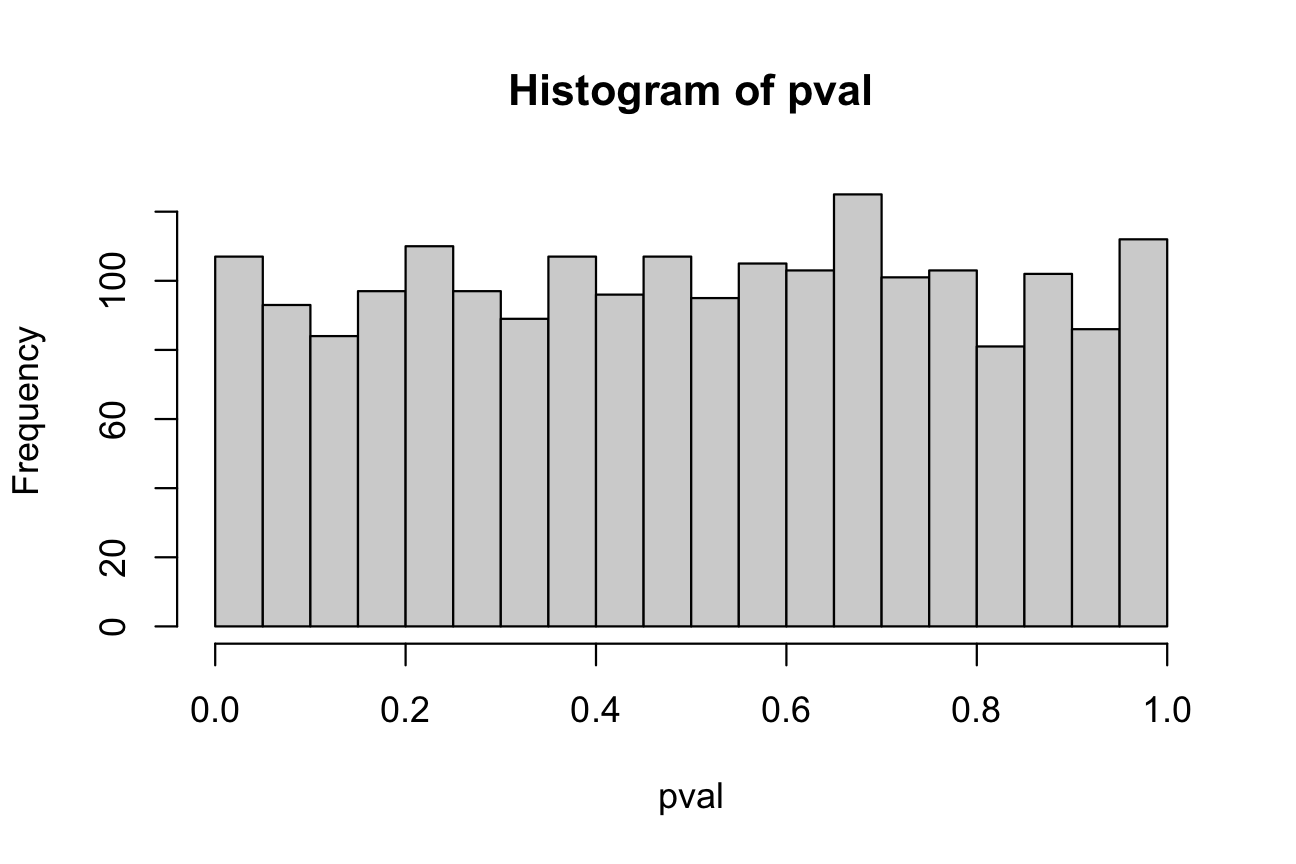
\includegraphics{Fig/unsupervised/unnamed-chunk-42-1} \end{center}


}

\normalsize

\scriptsize

\only<3>{


\begin{center}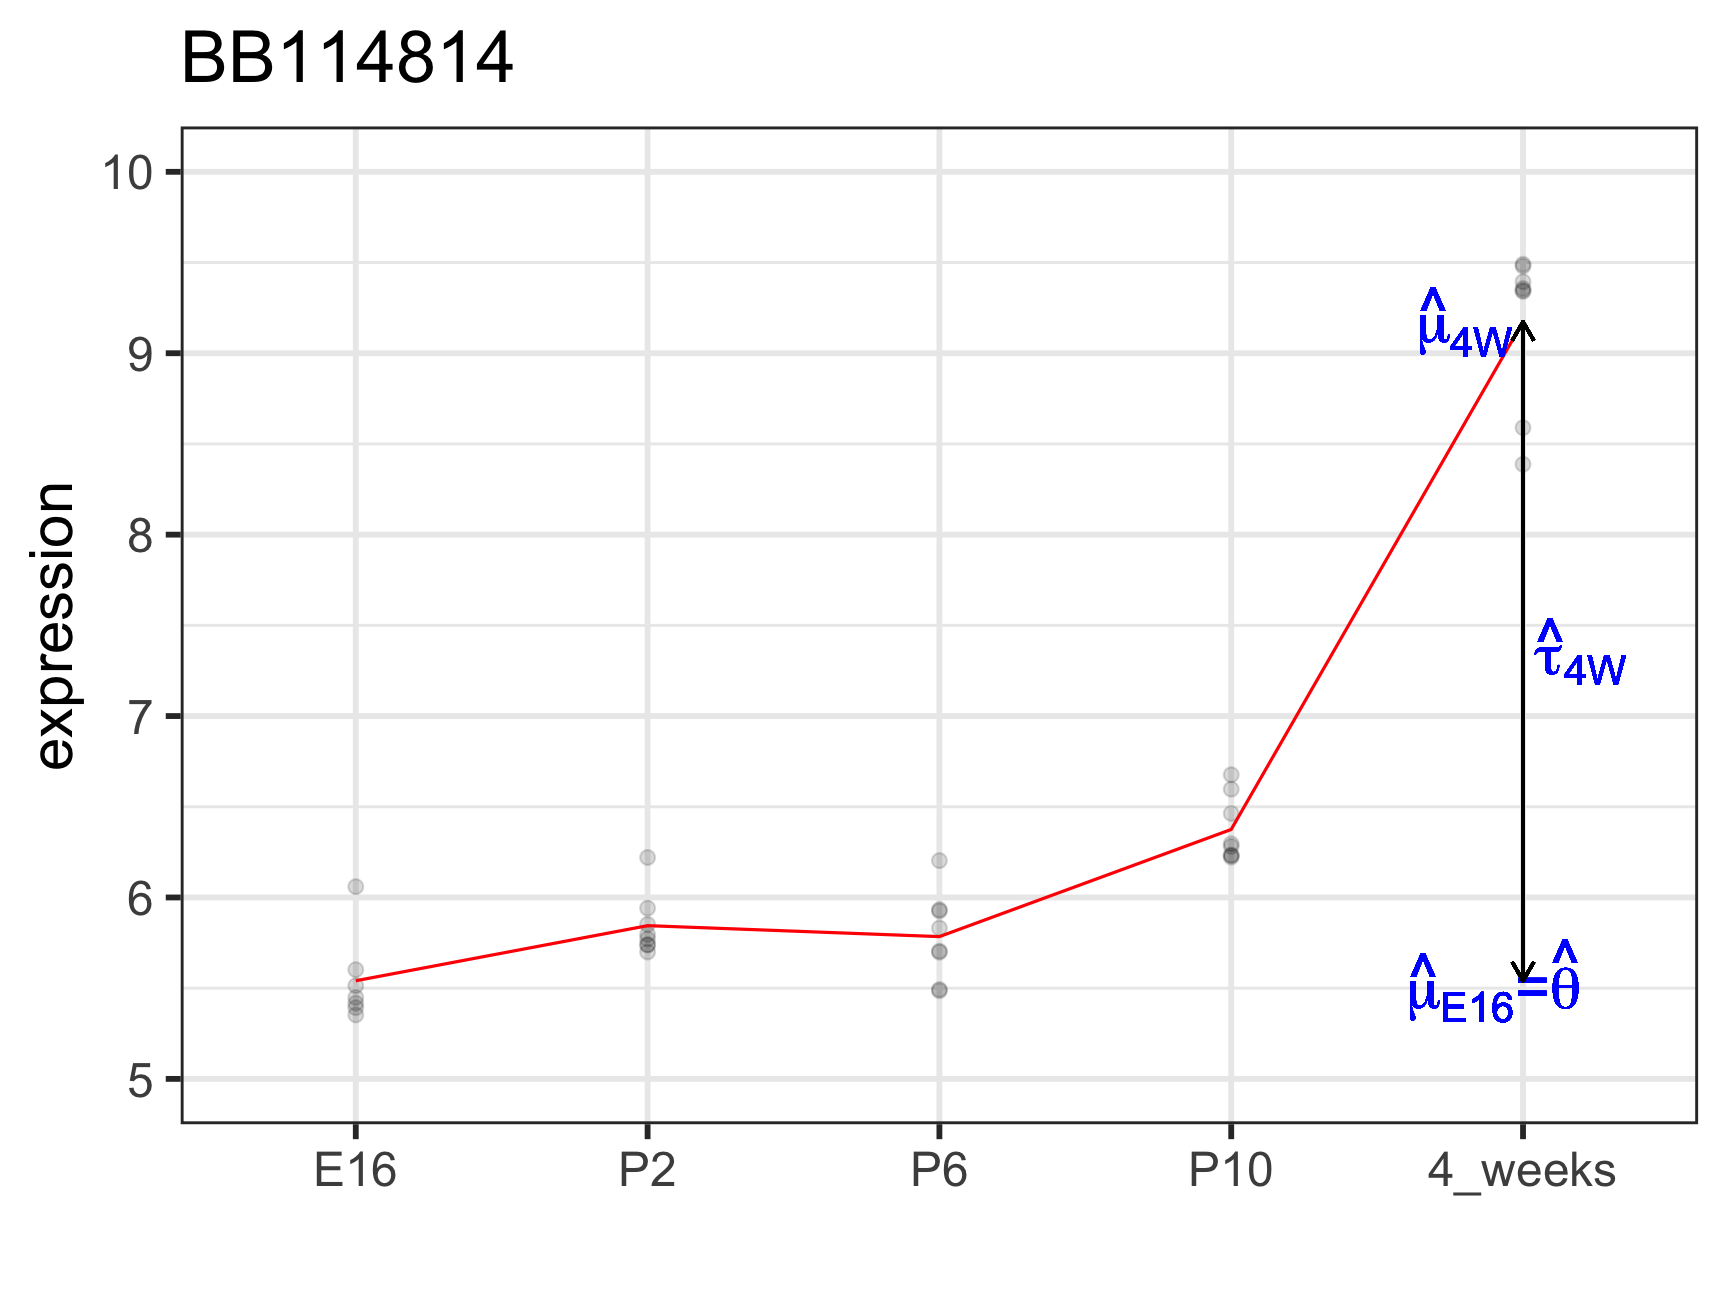
\includegraphics{Fig/unsupervised/unnamed-chunk-43-1} \end{center}


}

\normalsize
\end{column}

\begin{column}{.65\textwidth}
\scriptsize

\only<2>{


\begin{center}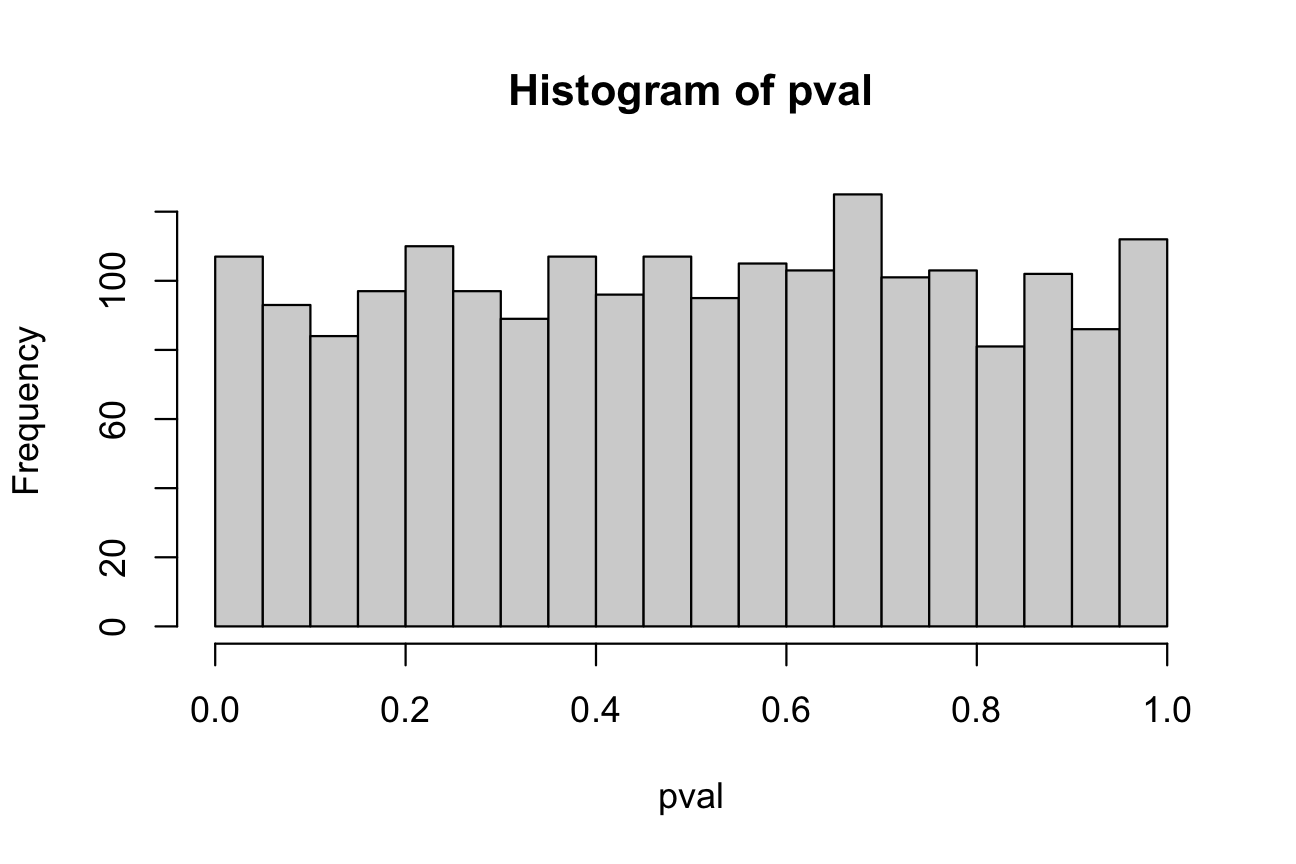
\includegraphics{Fig/unsupervised/unnamed-chunk-44-1} \end{center}


}

\normalsize

\scriptsize

\only<3>{


\begin{center}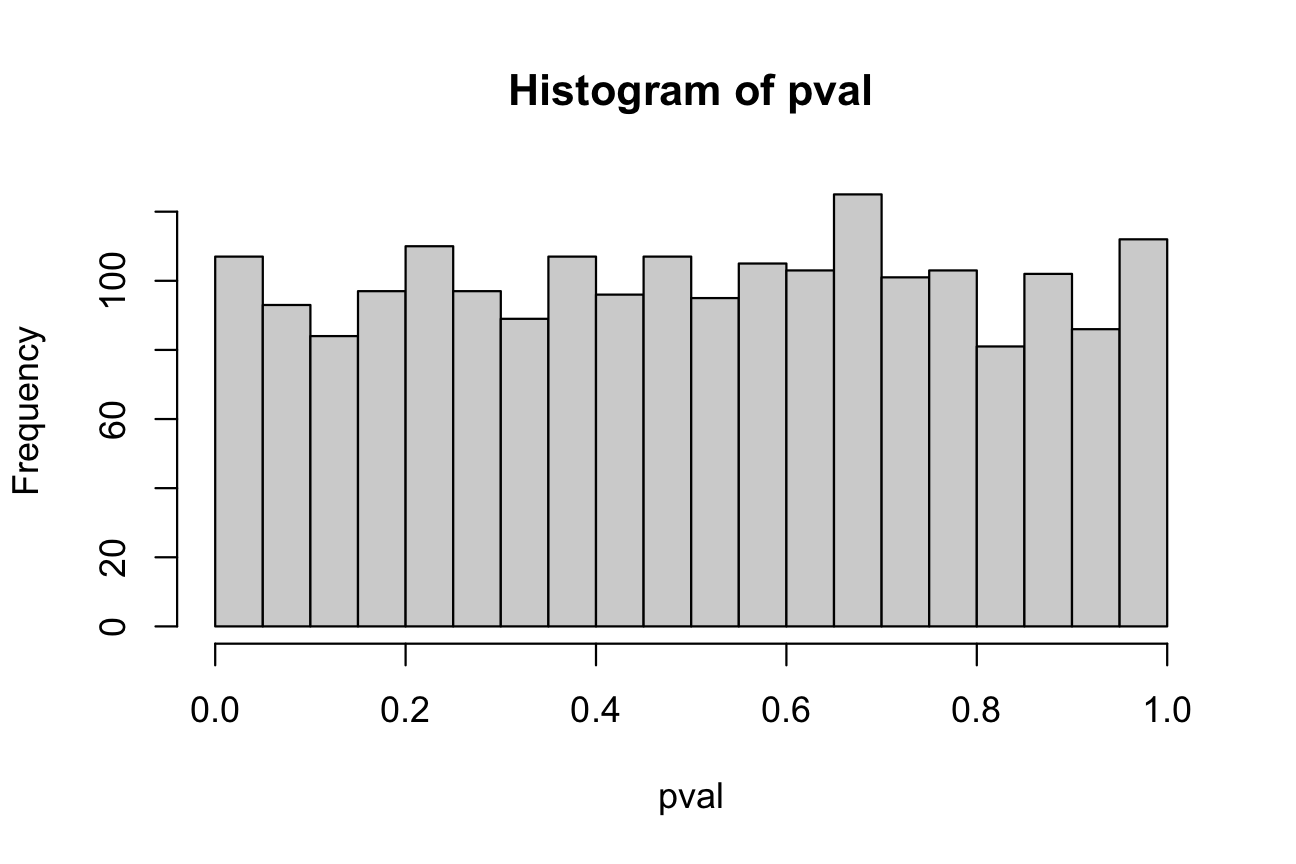
\includegraphics{Fig/unsupervised/unnamed-chunk-45-1} \end{center}


}

\normalsize
\end{column}
\end{columns}
\end{frame}

\begin{frame}{Can we find a set of ``good'' vectors to maximize the
explained variability?}
\protect\hypertarget{can-we-find-a-set-of-good-vectors-to-maximize-the-explained-variability}{}
\begin{block}{Recap: Sample covariance matrix}
\protect\hypertarget{recap-sample-covariance-matrix}{}
\begin{itemize}
\item
  Sample mean: \(\bar{X}_{i} = \sum_{j=1}^{m} X_{ji} / m\)
\item
  Sample variance: \(\sum_{j=1}^{m} (X_{ji} - \bar{X}_{i})^{2} / (m-1)\)
\item
  Sample covariance between \(i\) and \(k\):
  \[\frac{1}{m-1}\sum_{j=1}^{m} (X_{ji} - \bar{X}_{i}) (X_{jk} - \bar{X}_{k})\]
\end{itemize}
\end{block}

If all the column vectors \(\mathbf{x}_{i}\) are standardized, the
column-by-column covariance \(X^{\top}X / (m-1)\).

If all the row vectors \(\mathbf{x}_{d}\) are standardized, the
row-by-row covariance \(X X^{\top} / (n-1)\).
\end{frame}

\begin{frame}{Total variance of the projected data}
\protect\hypertarget{total-variance-of-the-projected-data}{}
\begin{columns}[T]
\begin{column}{.45\textwidth}
\begin{block}{Total variance}
\protect\hypertarget{total-variance}{}
Given the projected,
\(\hat{X} = \mathbf{u}_{1} \cdot (W_{11},\ldots,W_{1n})\), our goal is

\[\max \mathbb{V}\!\left[\hat{X}\right]\]
\end{block}

\begin{itemize}
\item
  We have two unknown variables \(U\) and \(W\)
\item
  There are an infinite number of solutions.
\end{itemize}
\end{column}

\begin{column}{.45\textwidth}
\begin{block}{Constrained total variance}
\protect\hypertarget{constrained-total-variance}{}
Given the projected, \(\hat{X} = \mathbf{u}_{1} \mathbf{w}\), and a unit
vector, namely \(\|\mathbf{u}_{1}\|=1\), our goal is equivalent to

\[\max \mathbf{u}^{\top} X X^{\top} \mathbf{u}\]
\end{block}

Because each \(\hat{W}_{i}\) is the solution to the least-square
problem:
\[\hat{W}_{i} = \arg\min \|\mathbf{x}_{i} - \mathbf{u} W_{i}\|\] by
solving the least square:
\[\hat{W}_{i} = \mathbf{x}_{i}^{\top}\mathbf{u} / \mathbf{u}^{\top}\mathbf{u},\,\forall i\]
\end{column}
\end{columns}
\end{frame}

\begin{frame}{Principal Component Analysis as an eigen value problem}
\protect\hypertarget{principal-component-analysis-as-an-eigen-value-problem}{}
\begin{columns}[T]
\begin{column}{.45\textwidth}
\begin{block}{PCA}
\protect\hypertarget{pca}{}
Letting the feature-by-feature sample covariance matrix
\(\hat{\Sigma} = XX^{\top}/(n-1)\), we want to find a unit vector
\(\mathbf{u}\) by

\[\max \mathbf{u}^{\top} \hat{\Sigma}\mathbf{u}\]

subject to \(\mathbf{u}^{\top}\mathbf{u} = 1\).
\end{block}
\end{column}

\begin{column}{.45\textwidth}
\begin{block}{Eigen value problem}
\protect\hypertarget{eigen-value-problem}{}
Given the covariance matrix \(\hat{\Sigma}\), we can resolve an
eigen-value \(\lambda\) and the corresponding eigen-vector
\(\mathbf{u}\) such that

\[\hat{\Sigma}\mathbf{u} = \lambda \mathbf{u}\]

(``eigen'' mean ``own'' in German).
\end{block}
\end{column}
\end{columns}

\emph{Why are they equivalent?} Solving the PCA problem is \ldots{}

\[\iff \max \underbrace{\mathbf{u}^{\top}\hat{\Sigma}\mathbf{u}}_{\textsf{total variation}} + \underbrace{\lambda\left(1 - \mathbf{u}^{\top}\mathbf{u}\right)}_{\textsf{constraint}},\,\lambda >0\,\quad\textsf{a.k.a. Lagrangian}\]

Taking the derivative with respect to \(\mathbf{u}\) and setting it to
zero, we get the eigen-value problem.
\end{frame}

\begin{frame}{Let's see how much the first eigenvector can explain}
\protect\hypertarget{lets-see-how-much-the-first-eigenvector-can-explain}{}
\begin{columns}[T]
\begin{column}{.35\textwidth}
\scriptsize

\only<1>{


\begin{center}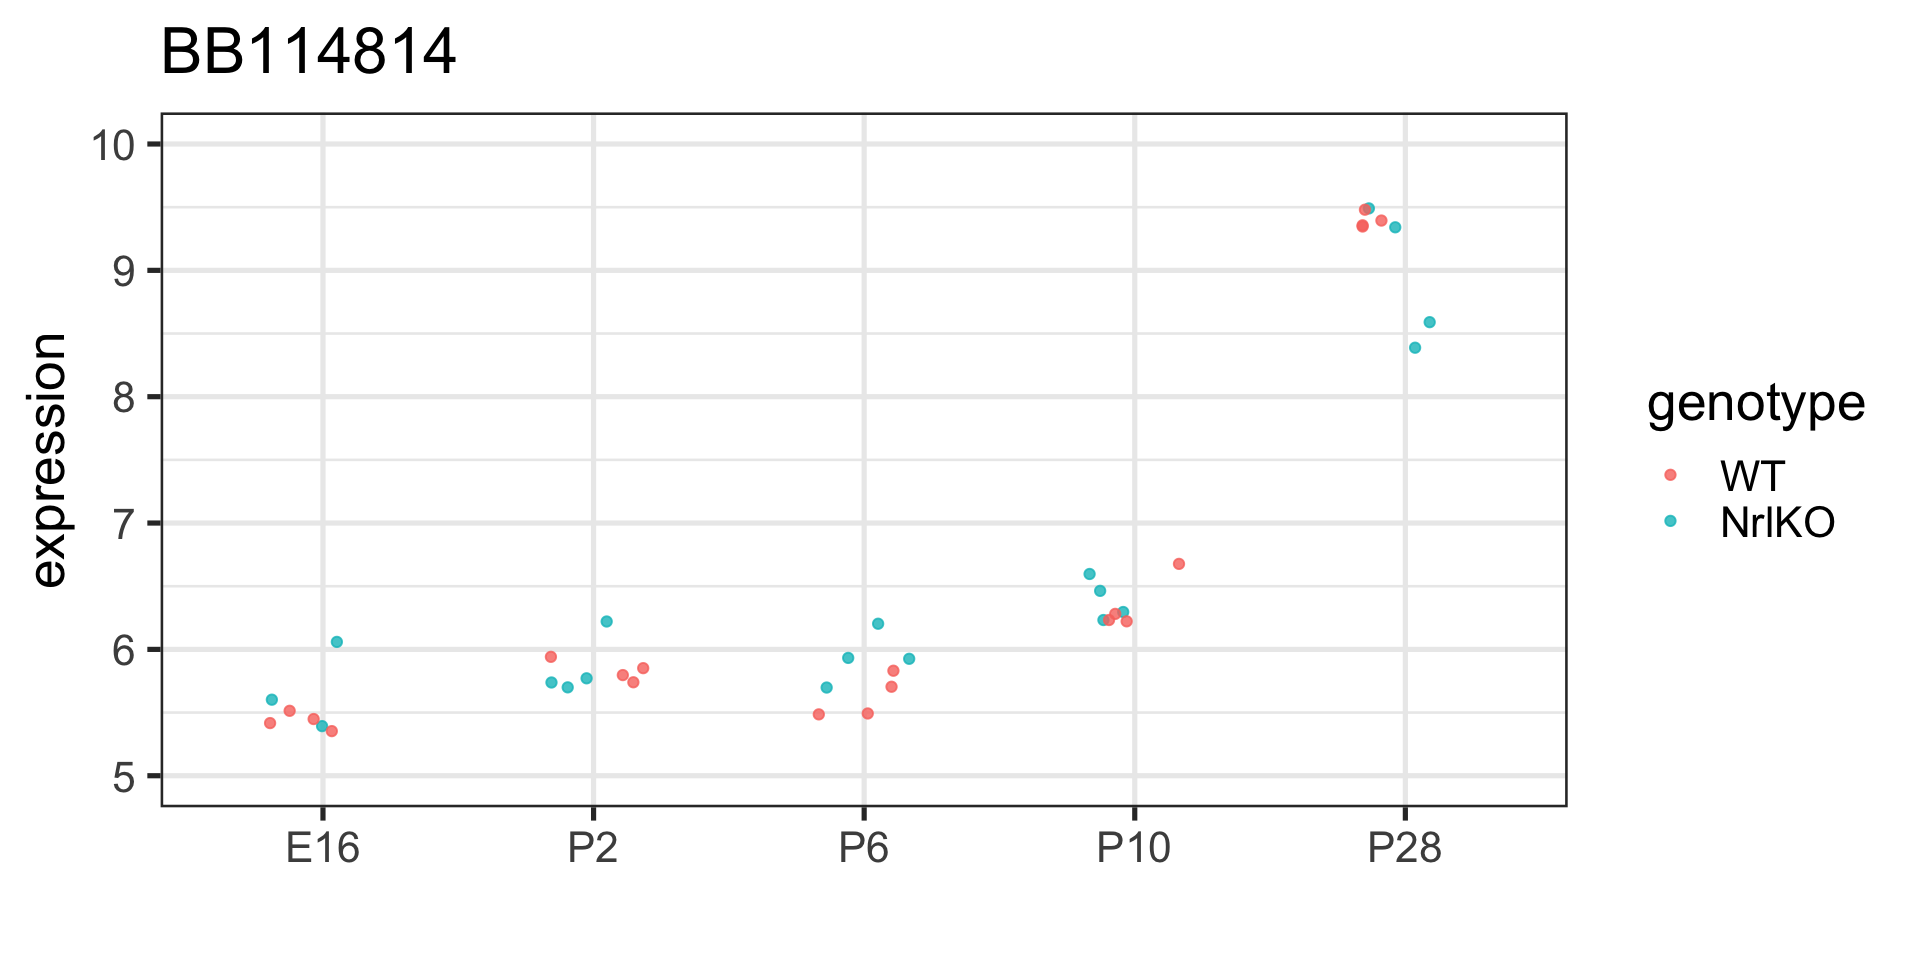
\includegraphics{Fig/unsupervised/unnamed-chunk-46-1} \end{center}


}

\normalsize

\scriptsize

\normalsize

\scriptsize

\only<2>{


\begin{center}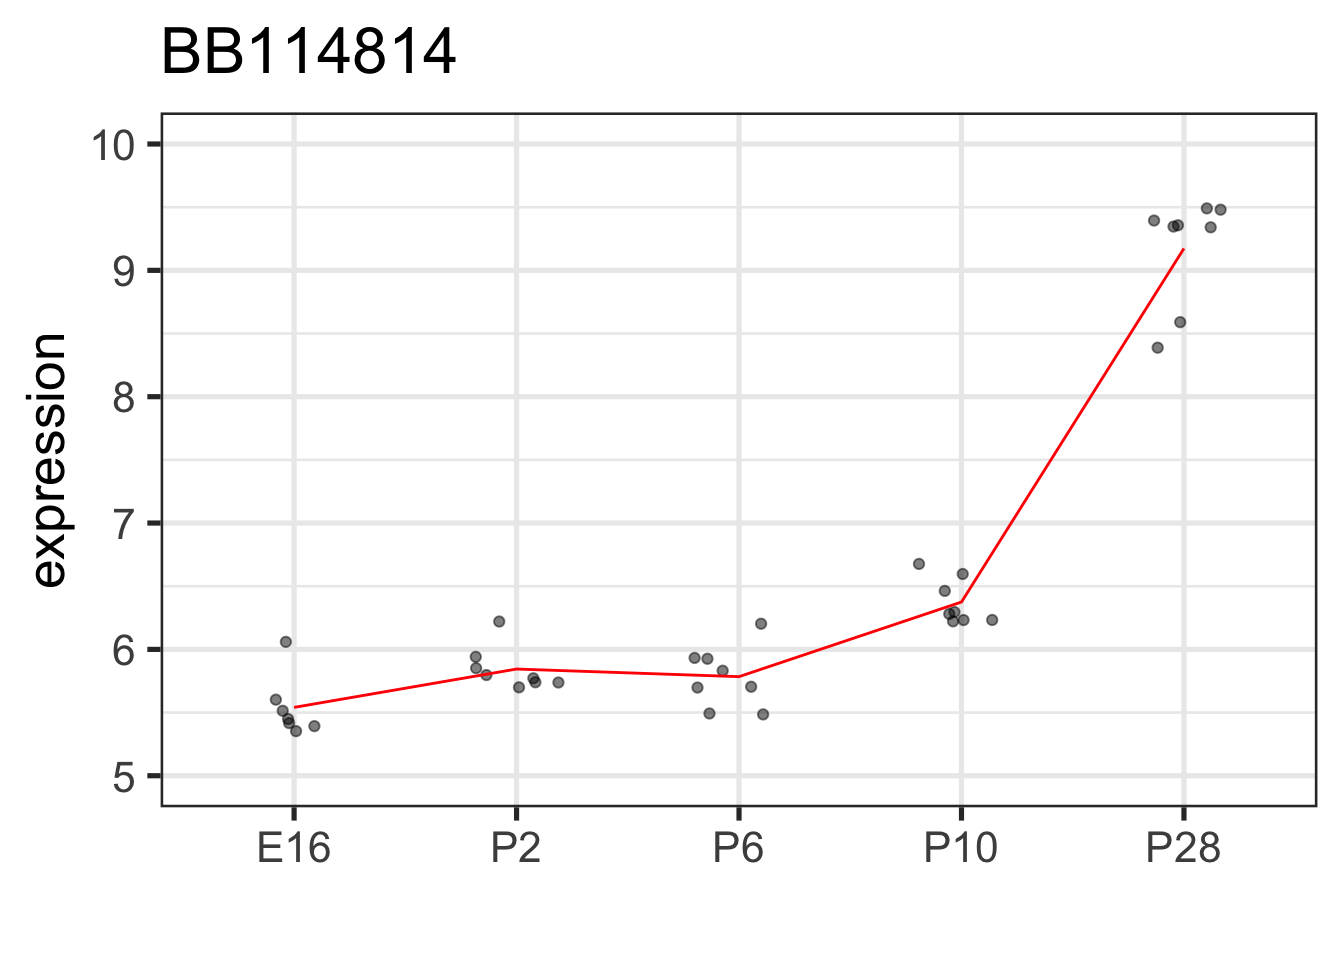
\includegraphics{Fig/unsupervised/unnamed-chunk-48-1} \end{center}


}

\normalsize

\scriptsize

\only<3>{


\begin{center}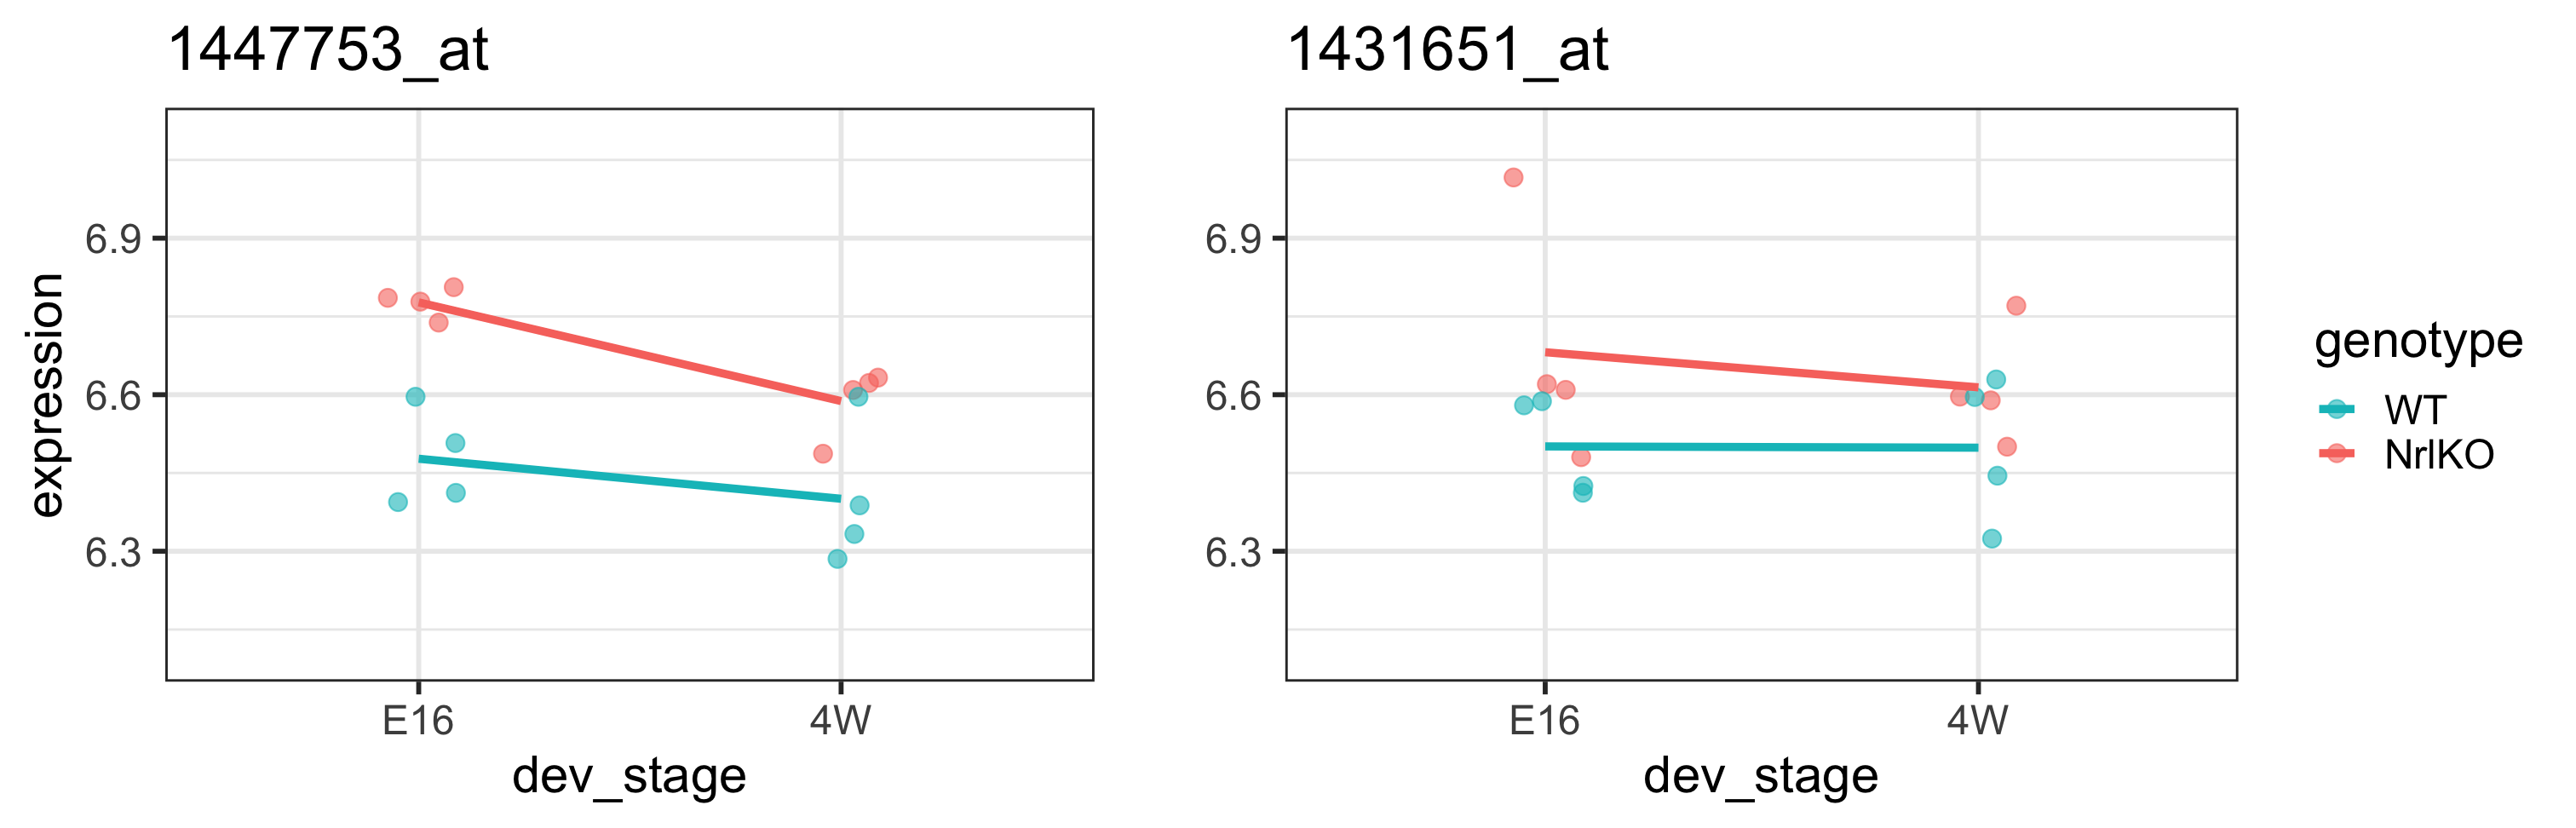
\includegraphics{Fig/unsupervised/unnamed-chunk-49-1} \end{center}


}

\normalsize
\end{column}

\begin{column}{.65\textwidth}
\scriptsize

\only<2>{


\begin{center}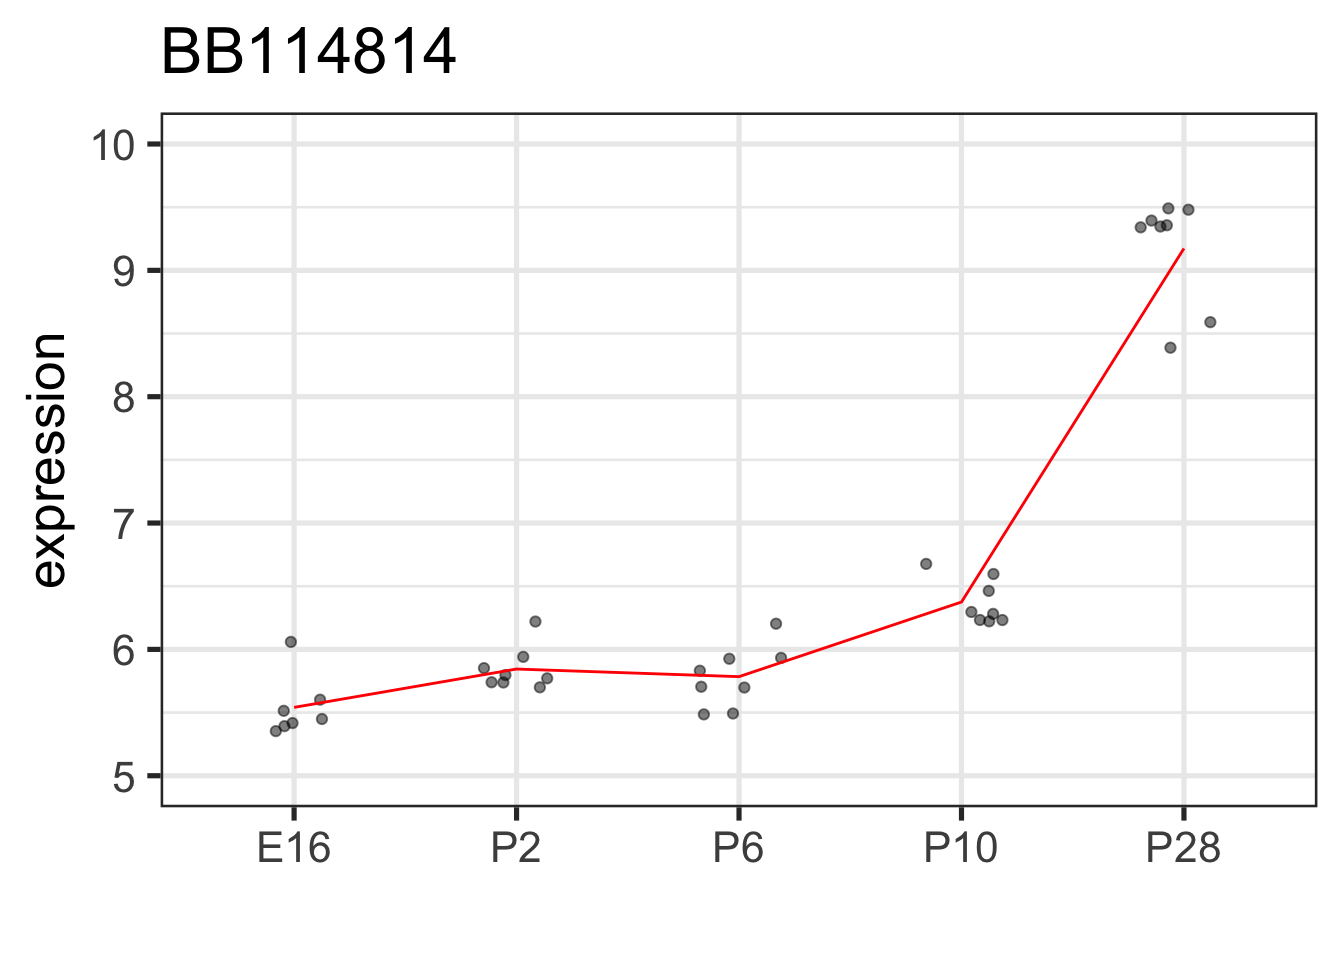
\includegraphics{Fig/unsupervised/unnamed-chunk-50-1} \end{center}


}

\normalsize

\scriptsize

\only<3>{


\begin{center}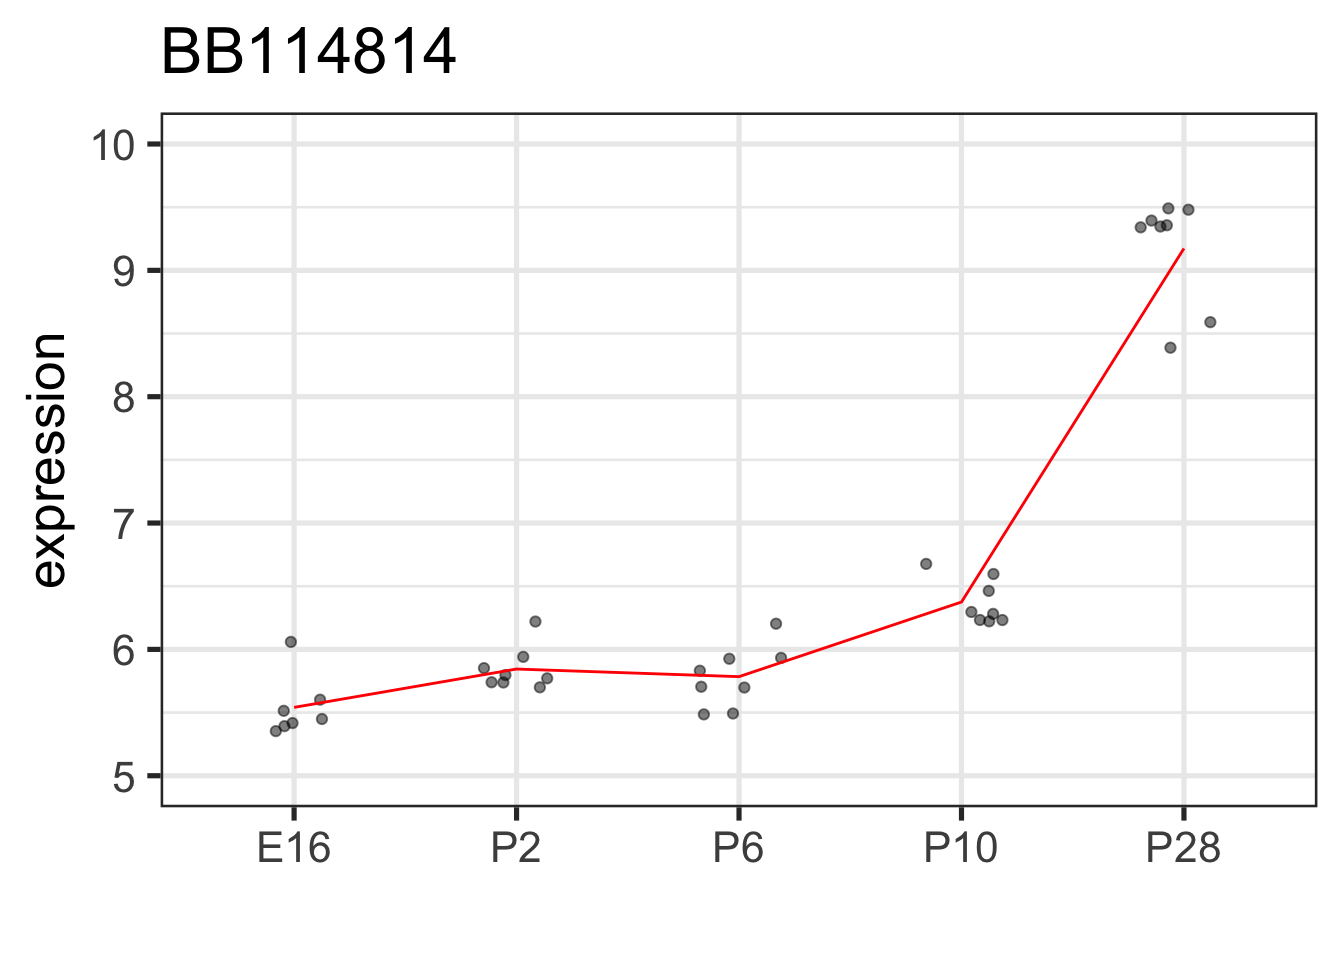
\includegraphics{Fig/unsupervised/unnamed-chunk-51-1} \end{center}


}

\normalsize
\end{column}
\end{columns}
\end{frame}

\begin{frame}{Top two eigen-vectors}
\protect\hypertarget{top-two-eigen-vectors}{}
\begin{columns}[T]
\begin{column}{.35\textwidth}
\scriptsize

\only<1>{


\begin{center}\includegraphics{Fig/unsupervised/unnamed-chunk-52-1} \end{center}


}

\normalsize

\scriptsize

\normalsize

\scriptsize

\only<2>{


\begin{center}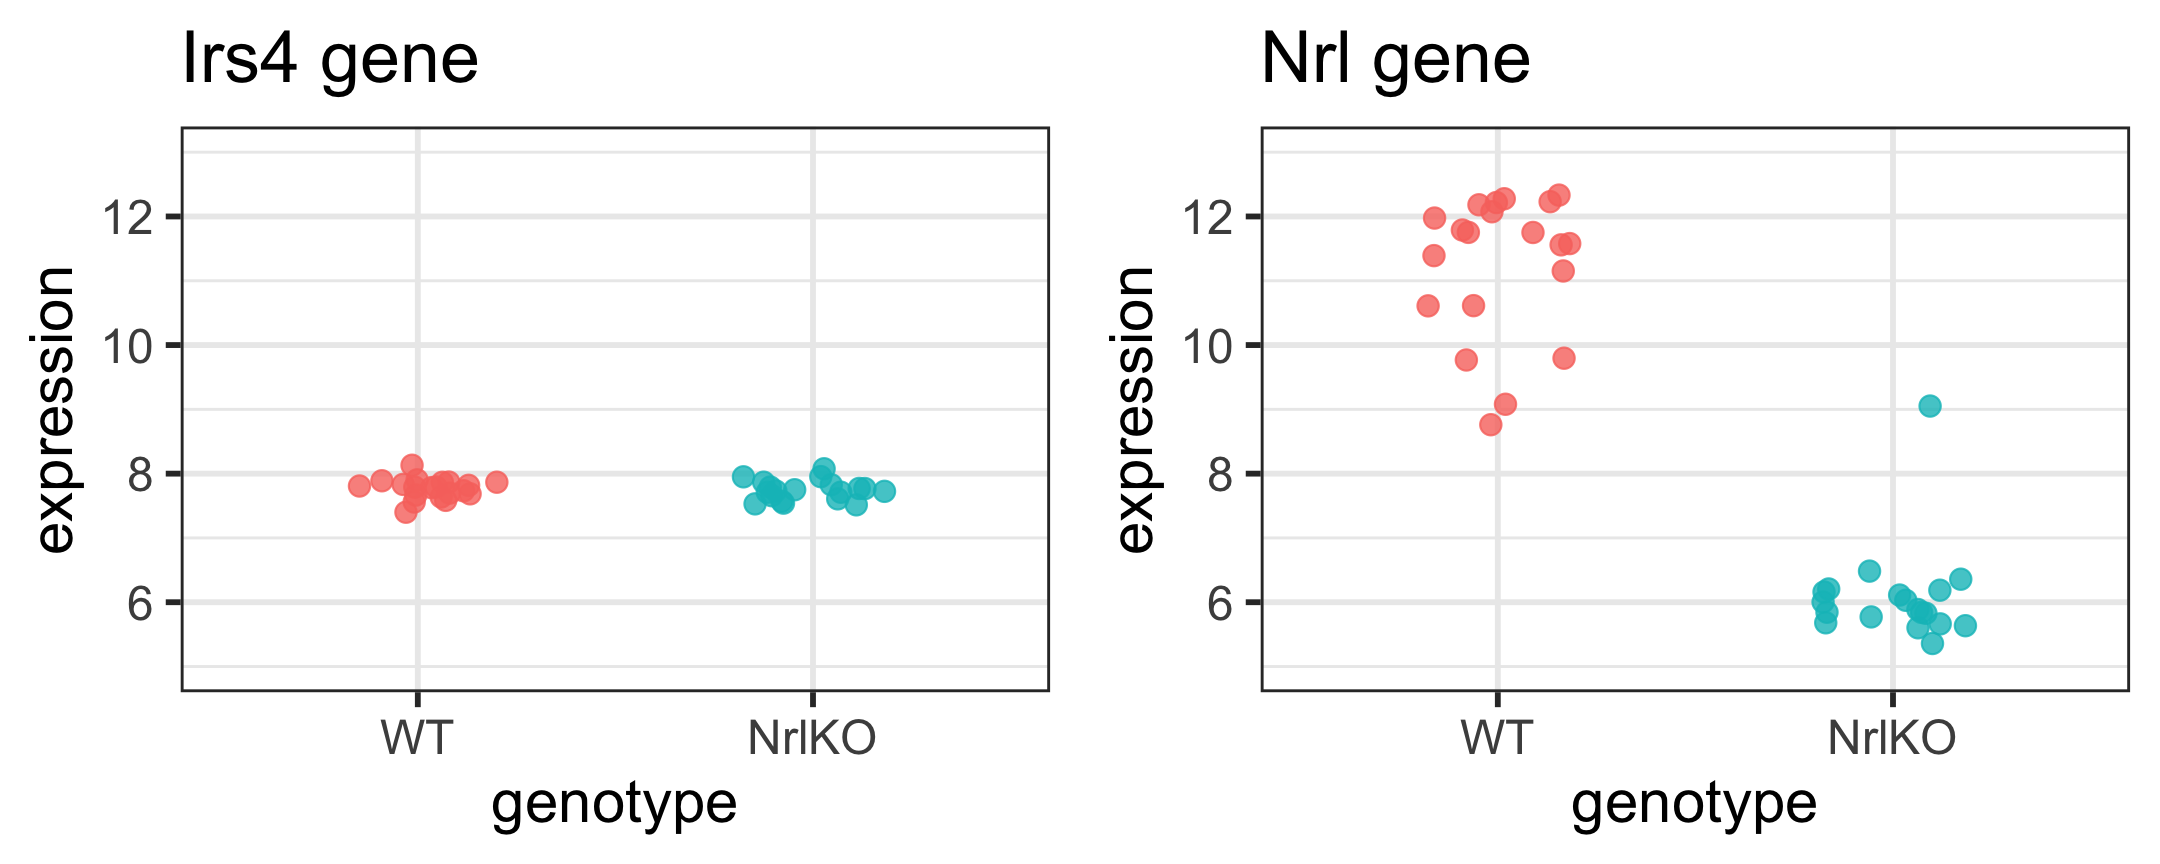
\includegraphics{Fig/unsupervised/unnamed-chunk-54-1} \end{center}


}

\normalsize

\scriptsize

\only<3>{


\begin{center}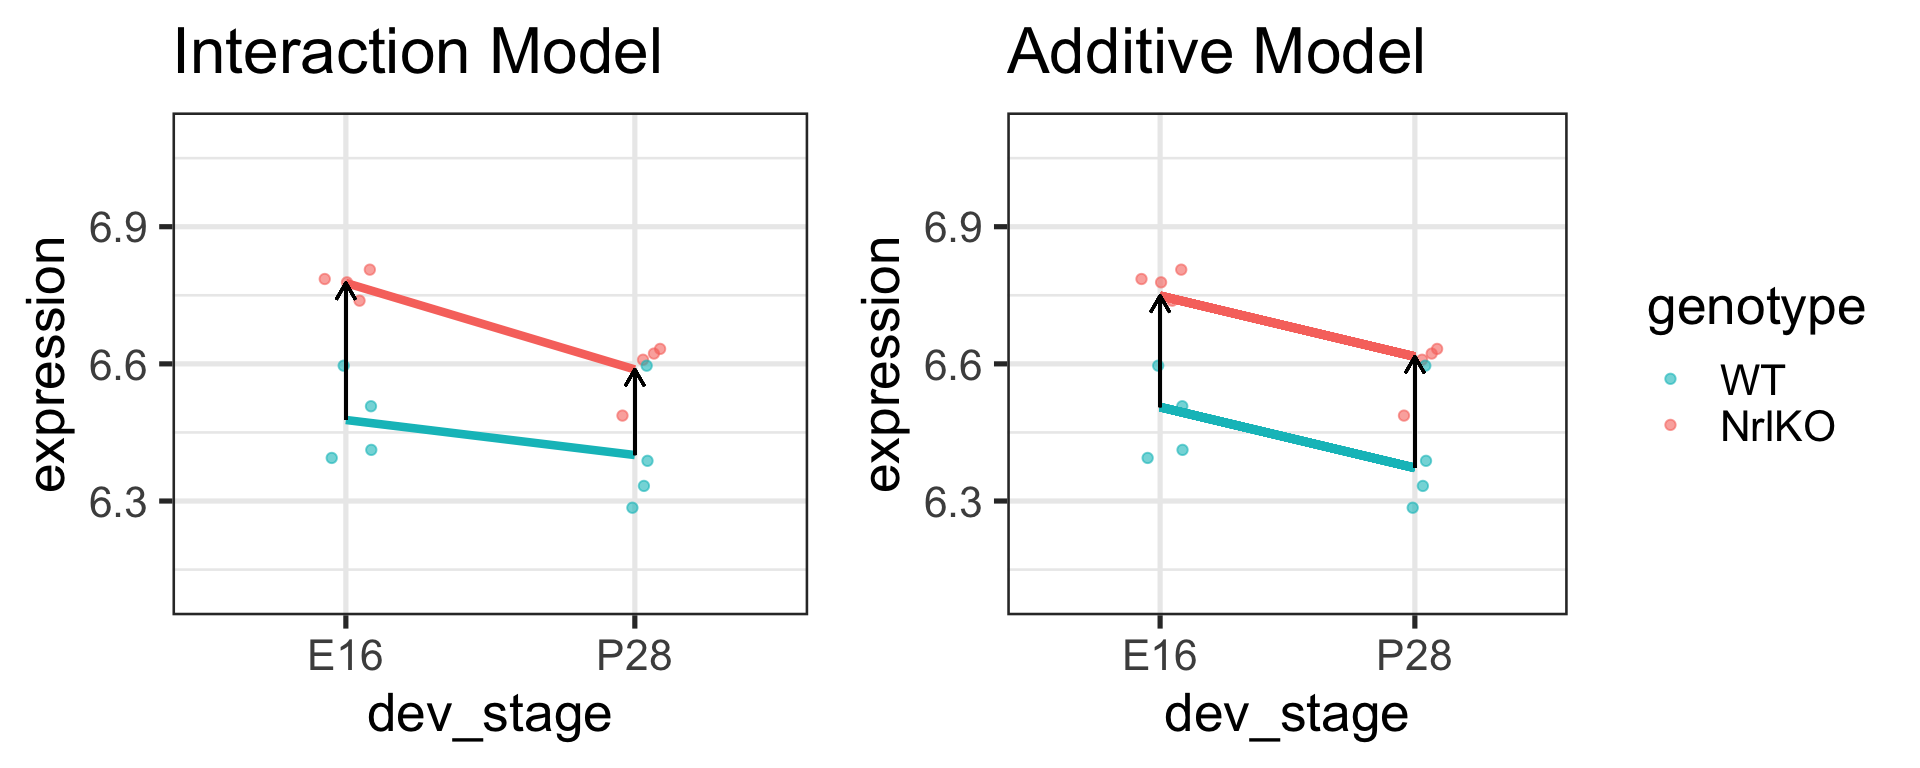
\includegraphics{Fig/unsupervised/unnamed-chunk-55-1} \end{center}


}

\normalsize
\end{column}

\begin{column}{.65\textwidth}
\scriptsize

\only<2>{


\begin{center}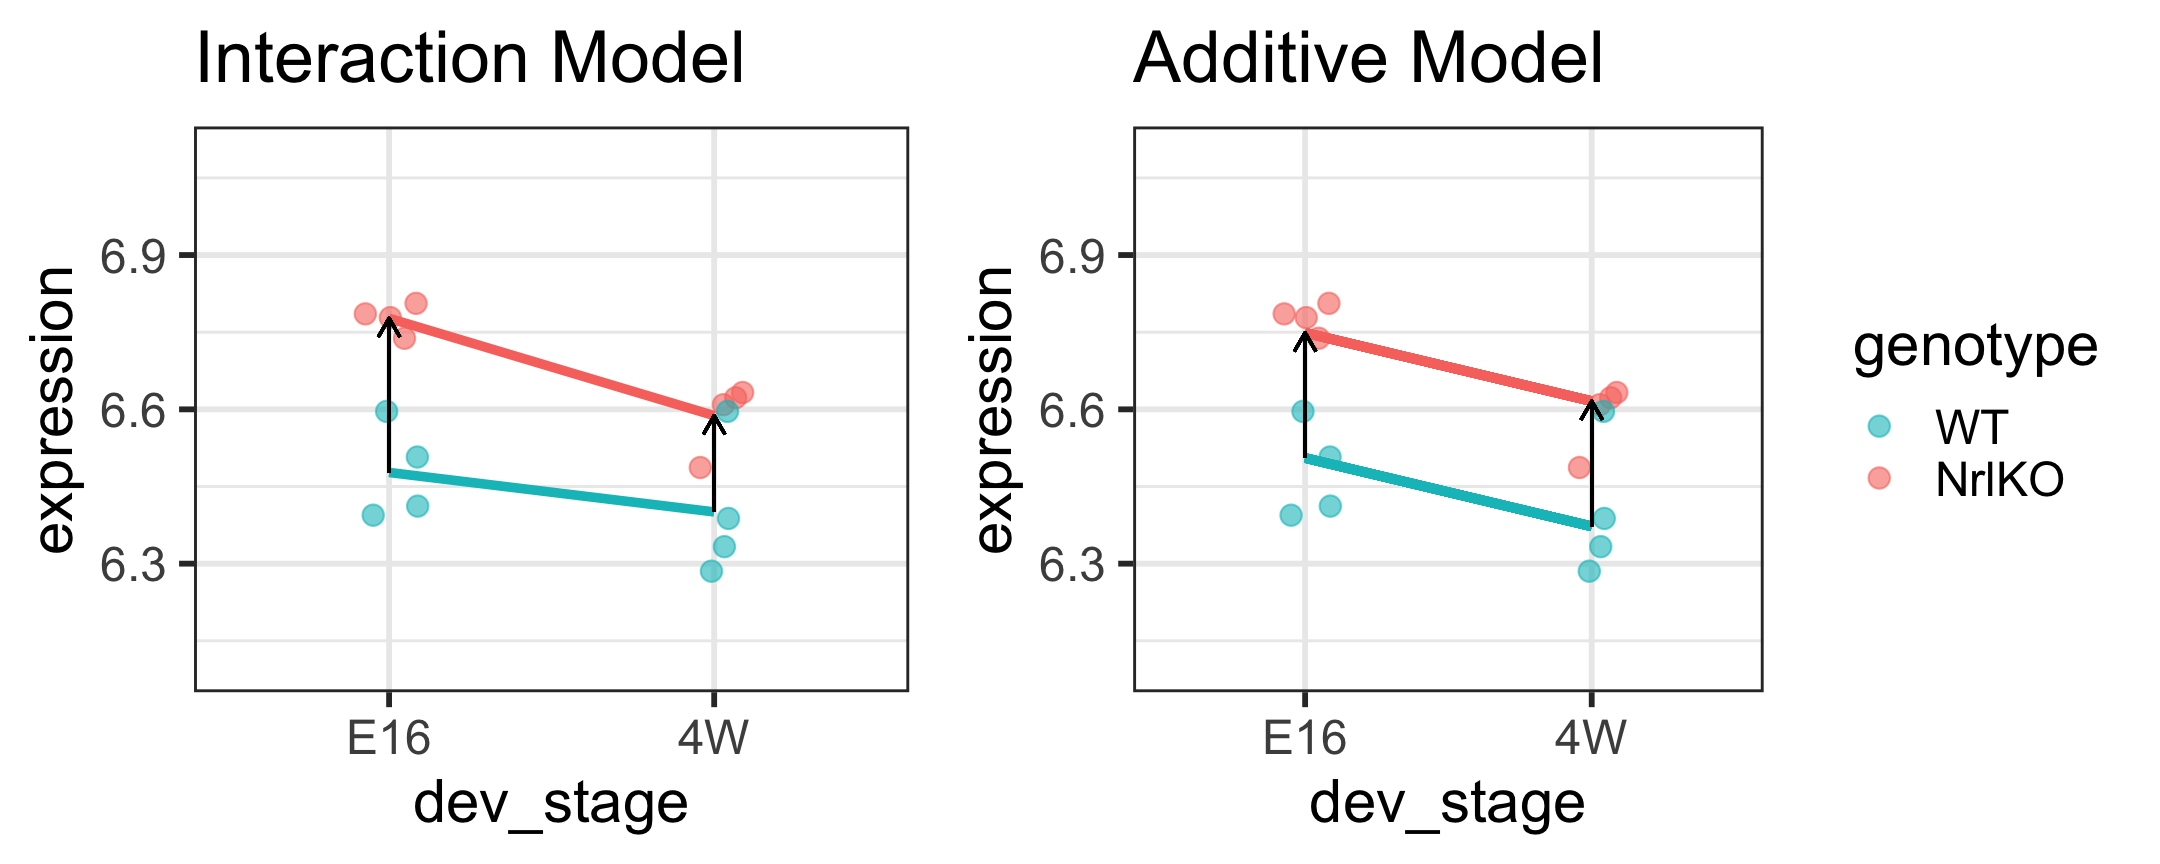
\includegraphics{Fig/unsupervised/unnamed-chunk-56-1} \end{center}


}

\normalsize

\scriptsize

\only<3>{


\begin{center}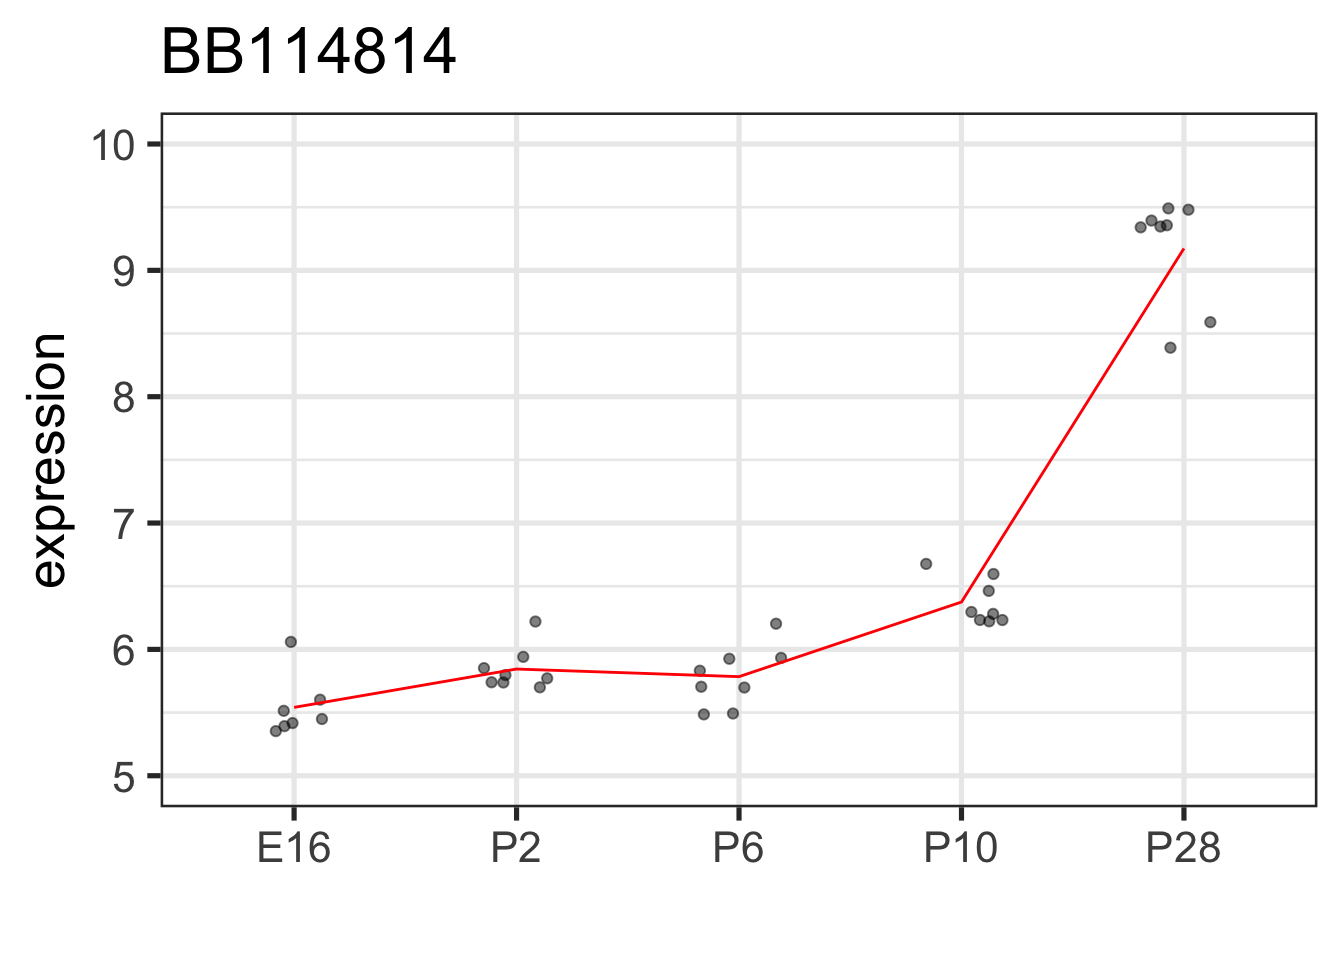
\includegraphics{Fig/unsupervised/unnamed-chunk-57-1} \end{center}


}

\normalsize
\end{column}
\end{columns}
\end{frame}

\begin{frame}{Top three eigen-vectors}
\protect\hypertarget{top-three-eigen-vectors}{}
\begin{columns}[T]
\begin{column}{.35\textwidth}
\scriptsize

\only<1>{


\begin{center}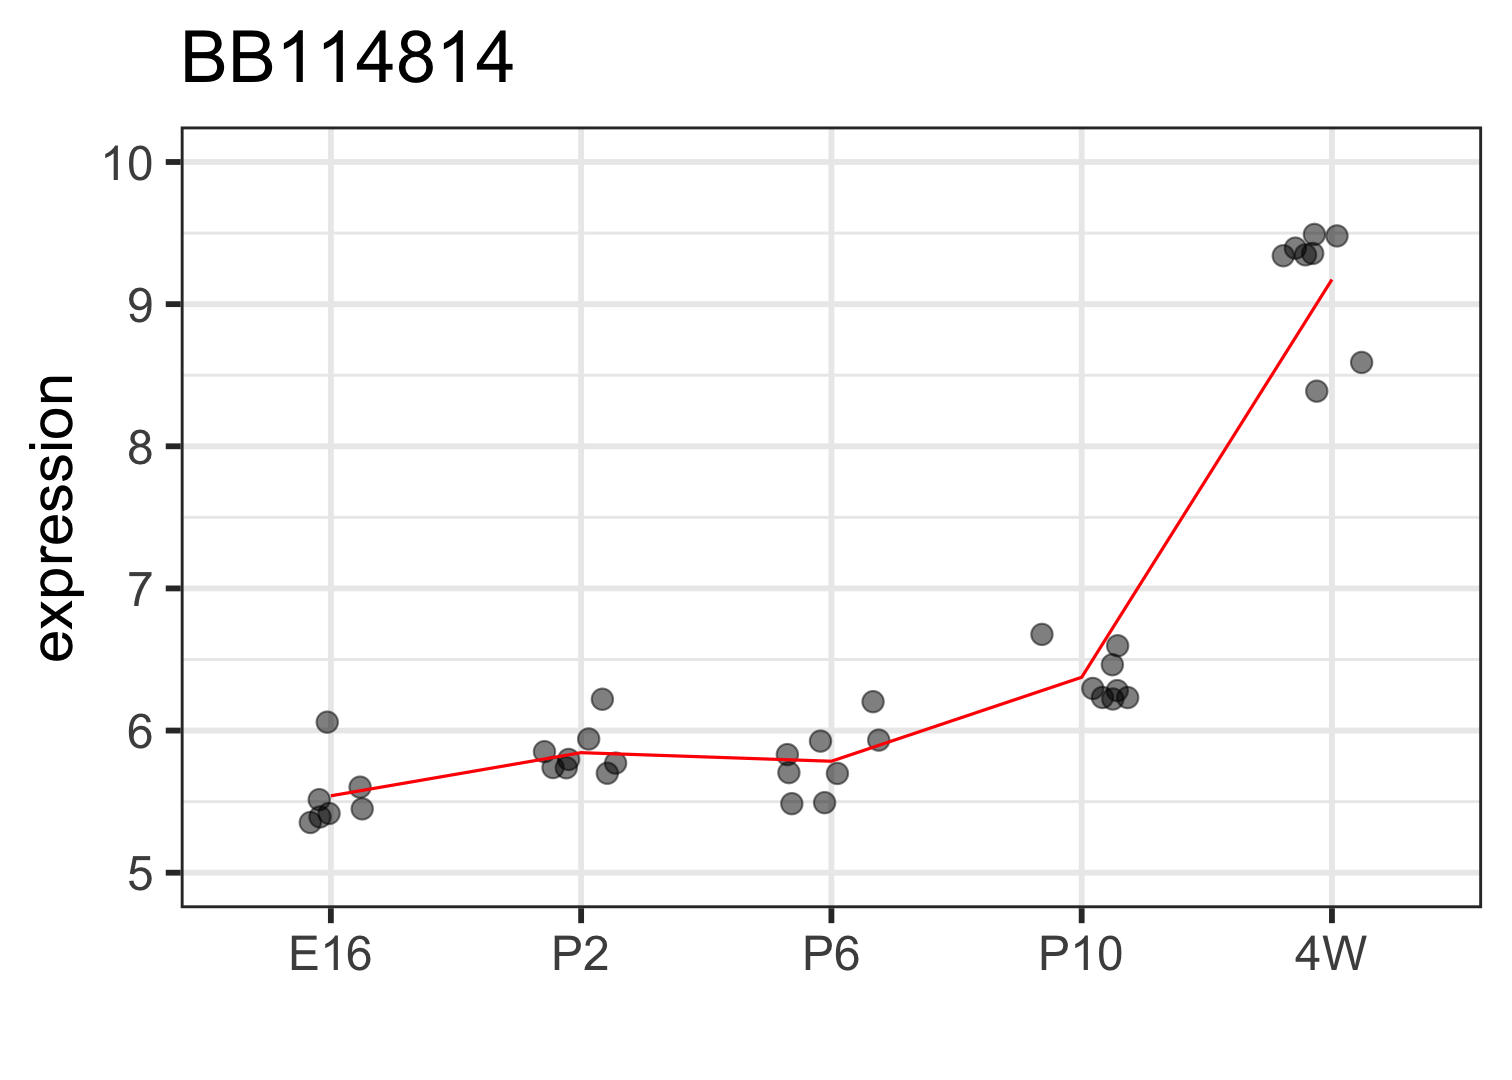
\includegraphics{Fig/unsupervised/unnamed-chunk-58-1} \end{center}


}

\normalsize

\scriptsize

\normalsize

\scriptsize

\only<2>{


\begin{center}\includegraphics{Fig/unsupervised/unnamed-chunk-60-1} \end{center}


}

\normalsize

\scriptsize

\only<3>{


\begin{center}\includegraphics{Fig/unsupervised/unnamed-chunk-61-1} \end{center}


}

\normalsize
\end{column}

\begin{column}{.65\textwidth}
\scriptsize

\only<2>{


\begin{center}\includegraphics{Fig/unsupervised/unnamed-chunk-62-1} \end{center}


}

\normalsize

\scriptsize

\only<3>{


\begin{center}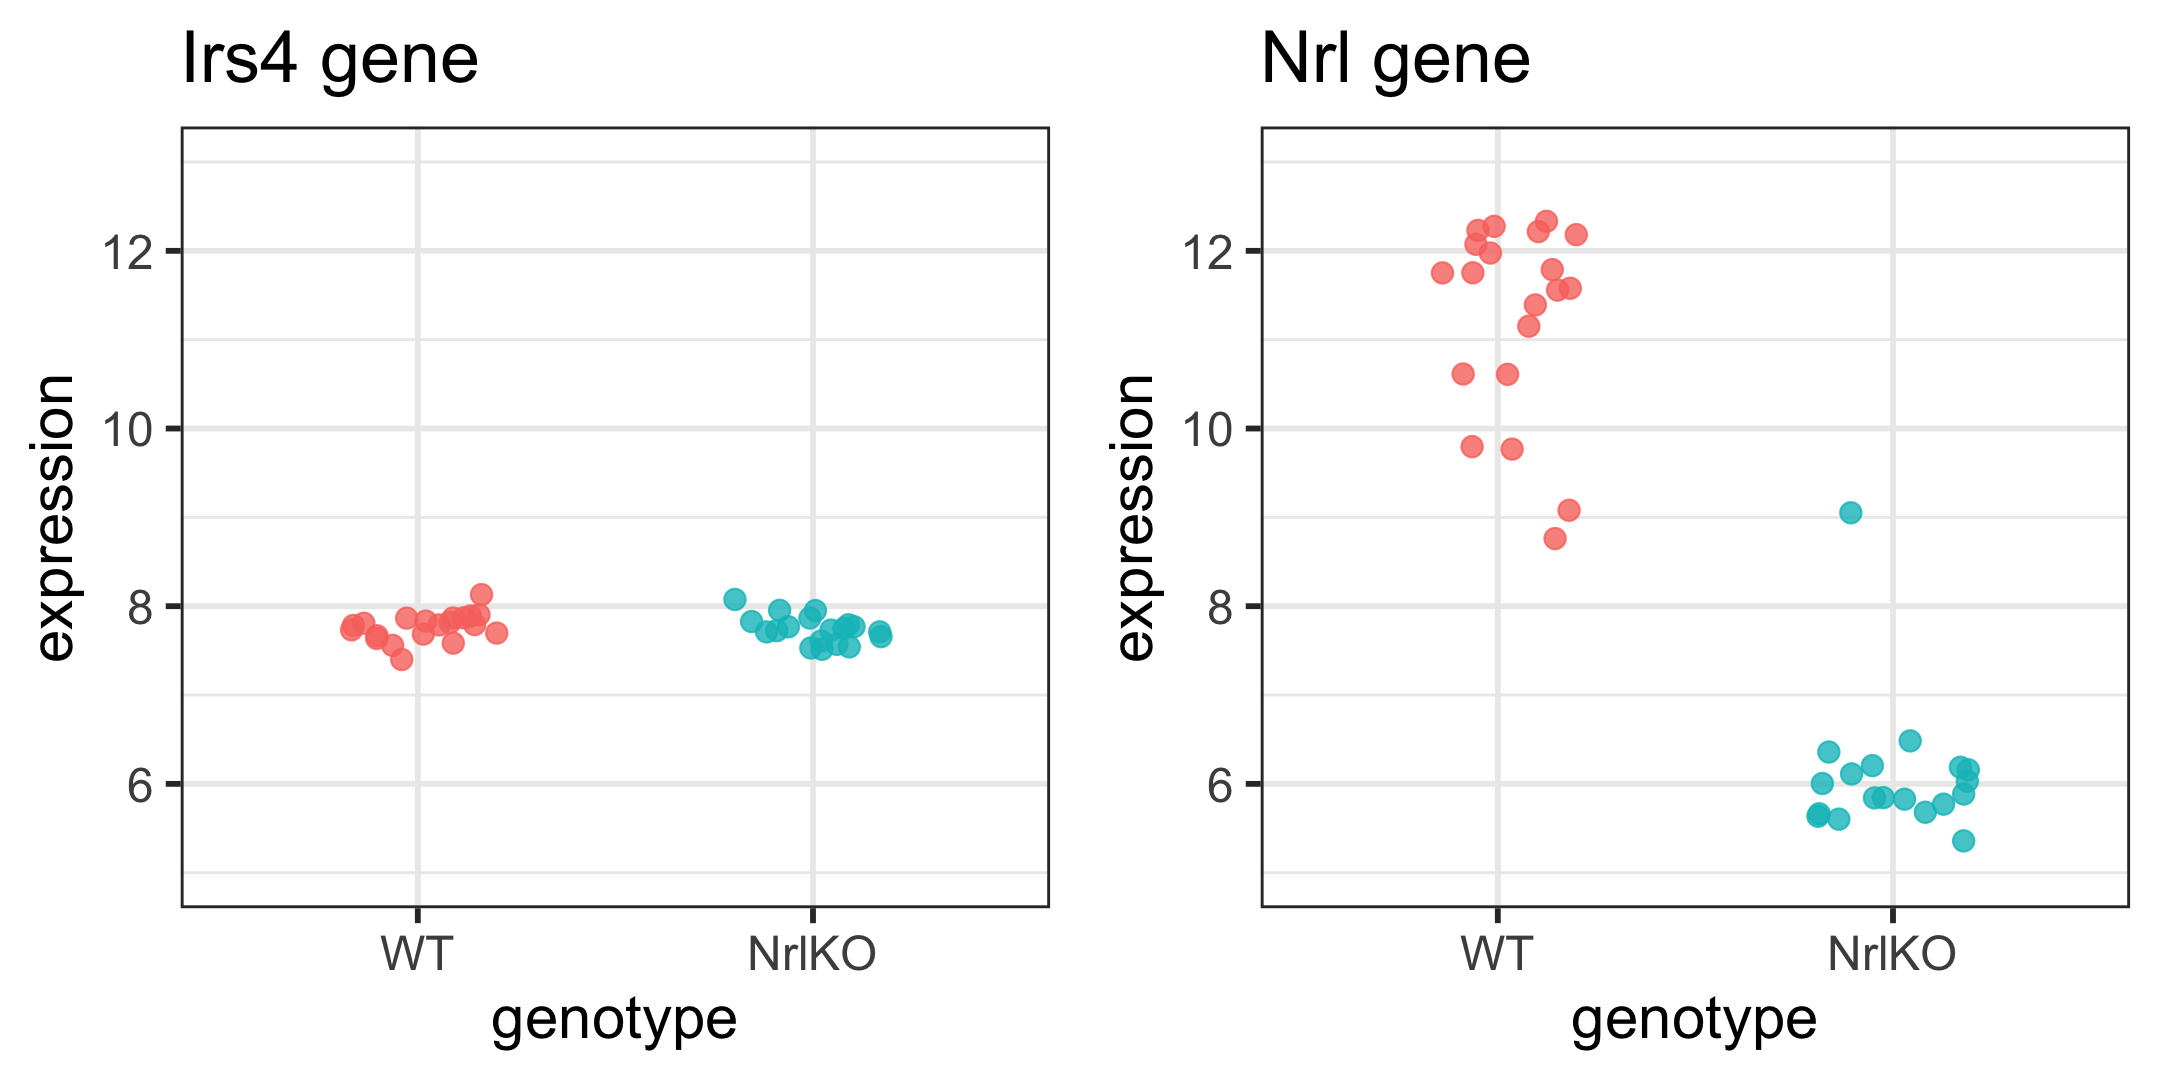
\includegraphics{Fig/unsupervised/unnamed-chunk-63-1} \end{center}


}

\normalsize
\end{column}
\end{columns}
\end{frame}

\begin{frame}{SVD: another equivalent method for PCA}
\protect\hypertarget{svd-another-equivalent-method-for-pca}{}
\begin{columns}[T]
\begin{column}{.45\textwidth}
\begin{block}{Singular Value Decomposition}
\protect\hypertarget{singular-value-decomposition}{}
SVD identifies three matrices of \(X\):

\[X = U D V^{\top}\]

where both \(U\) and \(V\) vectors are orthonormal, namely,

\begin{itemize}
\item
  \(U^{\top}U = I\), \(\mathbf{u}_{k}^{\top}\mathbf{u}_{k}=1\) for all
  \(k\),
\item
  \(V^{\top}V = I\), \(\mathbf{v}_{k}^{\top}\mathbf{v}_{k} = 1\) for all
  \(k\).
\end{itemize}
\end{block}
\end{column}

\begin{column}{.45\textwidth}
\begin{block}{Covariance by SVD}
\protect\hypertarget{covariance-by-svd}{}
Covariance across the columns (samples)

\[X^{\top}X/(m-1) = V D^{2} V^{\top}/(m-1)\]

Covariance across the rows (genes)

\[XX^{\top}/(n-1) = U D^{2} U^{\top}/(n-1)\]
\end{block}

\emph{Remark}: standardized matrix
\end{column}
\end{columns}
\end{frame}

\begin{frame}{SVD: another equivalent method for PCA}
\protect\hypertarget{svd-another-equivalent-method-for-pca-1}{}
We can confirm the equivalent relations by multiplying singular vectors
to the covariance matrix:

\begin{eqnarray*}
\onslide<1->{
    \underbrace{\left( \frac{1}{m-1} X^{\top}X \right)}_{\textsf{\color{blue} sample covariance}} \mathbf{v}_{1}
    &=& 
    \frac{1}{m-1} \left(\mathbf{v}_{1}, \mathbf{v}_{2},\ldots, \mathbf{v}_{k}\right)
      \left(
      \begin{array}{l l l l}
        D_{1}^{2} & 0 & \ldots & \ldots \\
        0 & D_{2}^{2} & 0 & \ldots \\
        0 & \ldots & \ddots & 0 \\
        0 & \ldots & 0 & D_{k}^{2} \\
      \end{array} \right)
  \left(
  \begin{array}{l}
    \mathbf{v}_{1}^{\top}\\
    \mathbf{v}_{2}^{\top}\\
    \vdots\\
    \mathbf{v}_{k}^{\top}
  \end{array}
  \right)
  \mathbf{v}_{1} \\
    }
    \onslide<2->{
  &=&
      \frac{1}{m-1} \left(\mathbf{v}_{1}, \mathbf{v}_{2},\ldots, \mathbf{v}_{k}\right)
      \left(
      \begin{array}{l l l l}
        D_{1}^{2} & 0 & \ldots & \ldots \\
        0 & D_{2}^{2} & 0 & \ldots \\
        0 & \ldots & \ddots & 0 \\
        0 & \ldots & 0 & D_{k}^{2} \\
      \end{array} \right)
  \left(
  \begin{array}{l}
    1 \\
    0 \\
    \vdots\\
    0
  \end{array}
  \right) \\
  }
\onslide<3->{
  &=&
      \frac{1}{m-1} \left(\mathbf{v}_{1}, \mathbf{v}_{2},\ldots, \mathbf{v}_{k}\right)
      \left(
      \begin{array}{l}
        D_{1}^{2} \\
        0 \\
        0 \\
        0 \\
      \end{array} \right)}
      \onslide<4>{
      =
  \underbrace{\frac{D_{1}^{2}}{m-1}}_{\textsf{\color{red}eigenvalue}}
  \underbrace{\mathbf{v}_{1}}_{\textsf{\color{red}eigenvector}}
  }
\end{eqnarray*}
\end{frame}

\begin{frame}[fragile]{Run SVD to find many principal components}
\protect\hypertarget{run-svd-to-find-many-principal-components}{}
\large

\begin{Shaded}
\begin{Highlighting}[]
\NormalTok{svd.out }\OtherTok{\textless{}{-}} \FunctionTok{svd}\NormalTok{(x.sub, }\AttributeTok{nu =} \DecValTok{5}\NormalTok{, }\AttributeTok{nv =} \DecValTok{5}\NormalTok{)}
\NormalTok{U }\OtherTok{\textless{}{-}}\NormalTok{ svd.out}\SpecialCharTok{$}\NormalTok{u; D }\OtherTok{\textless{}{-}} \FunctionTok{diag}\NormalTok{(svd.out}\SpecialCharTok{$}\NormalTok{d[}\DecValTok{1}\SpecialCharTok{:}\DecValTok{5}\NormalTok{]); V }\OtherTok{\textless{}{-}}\NormalTok{ svd.out}\SpecialCharTok{$}\NormalTok{v}
\end{Highlighting}
\end{Shaded}

\normalsize

\begin{columns}[T]
\begin{column}{.25\textwidth}
\scriptsize

\begin{center}\includegraphics{Fig/unsupervised/unnamed-chunk-65-1} \end{center}

\normalsize
\end{column}

\begin{column}{.65\textwidth}
\scriptsize

\begin{center}\includegraphics{Fig/unsupervised/unnamed-chunk-66-1} \end{center}

\normalsize
\end{column}
\end{columns}
\end{frame}

\begin{frame}{(Co-)Variance decomposition}
\protect\hypertarget{co-variance-decomposition}{}
\[\hat{\Sigma} = X^{\top}X/(m-1)\]

\scriptsize

\begin{center}\includegraphics{Fig/unsupervised/unnamed-chunk-67-1} \end{center}

\normalsize
\end{frame}

\begin{frame}{(Co-)Variance decomposition}
\protect\hypertarget{co-variance-decomposition-1}{}
\scriptsize

\normalsize

\[\hat{\Sigma} = \frac{X^{\top}X}{m-1} = V \frac{D^{2}}{m-1} V^{\top} = \sum_{k=1} \lambda_{k} \mathbf{v}_{k} \mathbf{v}_{k}^{\top},\quad \lambda_{k}=\frac{D_{k}^{2}}{m-1}\]

\begin{columns}[T]
\begin{column}{.28\textwidth}
\scriptsize

\begin{center}\includegraphics{Fig/unsupervised/unnamed-chunk-69-1} \end{center}

\normalsize
\end{column}

\begin{column}{.75\textwidth}
\scriptsize

\begin{center}\includegraphics{Fig/unsupervised/unnamed-chunk-70-1} \end{center}

\normalsize

\begin{itemize}
\tightlist
\item
  How much variance is explained by each component?
\end{itemize}
\end{column}
\end{columns}
\end{frame}

\begin{frame}{Eigenvectors decompose total covariance}
\protect\hypertarget{eigenvectors-decompose-total-covariance}{}
\scriptsize

\only<1>{


\begin{center}\includegraphics{Fig/unsupervised/unnamed-chunk-71-1} \end{center}


}

\normalsize

\scriptsize

\only<2>{


\begin{center}\includegraphics{Fig/unsupervised/unnamed-chunk-72-1} \end{center}


}

\normalsize
\end{frame}

\hypertarget{clustering-to-uncover-common-features-and-hidden-groups}{%
\section{Clustering to uncover common features and hidden
groups}\label{clustering-to-uncover-common-features-and-hidden-groups}}

\begin{frame}{Clustering to uncover common features and hidden groups}
\scriptsize

\normalsize
\end{frame}

\begin{frame}{The goal of this clustering section}
\protect\hypertarget{the-goal-of-this-clustering-section}{}
\begin{itemize}
\item
  Model-based unsupervised learning

  \begin{itemize}
  \tightlist
  \item
    Latent variable model
  \end{itemize}
\item
  Expectation Maximization
\item
  Hands-on experience with clustering algorithm
\end{itemize}

\scriptsize

\normalsize
\end{frame}

\begin{frame}{What clustering can do: Find common patterns across rows
and columns}
\protect\hypertarget{what-clustering-can-do-find-common-patterns-across-rows-and-columns}{}
\scriptsize

\only<1>{


\begin{center}\includegraphics{Fig/unsupervised/unnamed-chunk-75-1} \end{center}


}

\normalsize

\scriptsize

\only<2->{


\begin{center}\includegraphics{Fig/unsupervised/unnamed-chunk-76-1} \end{center}


}

\normalsize
\end{frame}

\begin{frame}{Model-based clustering (if you were a Bayesian
statistician\ldots)}
\protect\hypertarget{model-based-clustering-if-you-were-a-bayesian-statistician}{}
\begin{columns}[T]
\begin{column}{.45\textwidth}
\begin{block}{Simulation/data generation}
\protect\hypertarget{simulationdata-generation}{}
\emph{Given a data generating process, what are the properties of the
outcomes?}
\end{block}
\end{column}

\begin{column}{.45\textwidth}
\begin{block}{Model inference}
\protect\hypertarget{model-inference}{}
\emph{Given the outcomes, what can we say about the process that
generated the data?}
\end{block}
\end{column}
\end{columns}

\scriptsize

\begin{center}\includegraphics[width=.7\linewidth]{./Vis/unsupervised/model_based_inference} \end{center}

\normalsize

\tiny

Wassermann, \emph{All of Statistics} (2004)

\scriptsize

\normalsize
\end{frame}

\begin{frame}{What do we want to know from data?}
\protect\hypertarget{what-do-we-want-to-know-from-data}{}
\scriptsize

\begin{center}\includegraphics{Fig/unsupervised/unnamed-chunk-79-1} \end{center}

\normalsize

\textbf{Two goals}: recover (1) group membership and (2) the centroids
(red marks)
\end{frame}

\begin{frame}{A chicken-and-egg problem: guessing latent membership
vs.~parametric inference}
\protect\hypertarget{a-chicken-and-egg-problem-guessing-latent-membership-vs.-parametric-inference}{}
\begin{itemize}
\item
  If we knew the membership of all the points, we can simply estimate
  the centre (e.g., taking sample mean within each cluster)
\item
  If we knew the centre coordinates, we would be able to assign points
  to most probable groups easily based on distance from the centre
  points.
\item
  Statistical answer: Solve the underlying inference problem.
\item
  To a parameter estimator, the membership assignments are \emph{hidden}
  (latent).
\end{itemize}

\scriptsize

\normalsize

\scriptsize

\normalsize
\end{frame}

\begin{frame}{Let's think about the data-generating process to
``reverse'' it}
\protect\hypertarget{lets-think-about-the-data-generating-process-to-reverse-it}{}
\begin{columns}[T]
\begin{column}{.5\textwidth}
\scriptsize

\begin{center}\includegraphics{Fig/unsupervised/unnamed-chunk-82-1} \end{center}

\normalsize
\end{column}

\begin{column}{.45\textwidth}
\begin{block}{Latent Variable Model}
\protect\hypertarget{latent-variable-model}{}
What could have been done to generate observe data?

\begin{itemize}
\item
  Latent membership: \(Z_{ik}\)
\item
  Model parameters: \(\mu_{k}\) and \(\sigma_{k}\)
\end{itemize}
\end{block}
\end{column}
\end{columns}
\end{frame}

\begin{frame}{Gaussian Mixture Model (k-means)}
\protect\hypertarget{gaussian-mixture-model-k-means}{}
\begin{columns}[T]
\begin{column}{.4\textwidth}
\scriptsize

\begin{center}\includegraphics[width=.7\linewidth]{./Vis/unsupervised/GMM_graphical_model} \end{center}

\normalsize
\end{column}

\begin{column}{.5\textwidth}
\begin{block}{GMM data generating process}
\protect\hypertarget{gmm-data-generating-process}{}
\begin{enumerate}
\item
  Initialize \(\mu_{k}\) (the centre of each group) and \(\sigma_{k}\)
  (the spread within each group)
\item
  Randomly assign group membership, \(Z_{ik} = 1\) iff a point \(i\)
  belongs to a group \(k\).
\item
  Generate:
  \(\mathbf{x}_{i} | Z_{ik} = 1, \boldsymbol{\mu}_{k} \sim \mathcal{N}\!\left(\boldsymbol{\mu}_{k}, \sigma^{2}I\right)\)
\end{enumerate}
\end{block}
\end{column}
\end{columns}

How do we infer \(Z\) and \(\mu,\sigma\)?
\end{frame}

\begin{frame}{}
\protect\hypertarget{section}{}
\includegraphics{Vis/unsupervised/EM_paper.jpg}
\end{frame}

\begin{frame}{Expectation Maximization for GMM MLE}
\protect\hypertarget{expectation-maximization-for-gmm-mle}{}
\begin{eqnarray*}
\onslide<1->{
    J &\equiv& \log \prod_{i=1}^{n} p(\mathbf{x}_{i}|\mu,\sigma) \\
}
\onslide<2>{
    &=& \log \prod_{i=1}^{n} \sum_{Z} p(\mathbf{x}_{i}|Z,\mu,\sigma)p(Z)
}
\end{eqnarray*}

\onslide<2>{
* It might be difficult to enumerate all the $Z$'s... so let's introduce some other distributions that will help our "guessing" work, which we call it $q(Z)$
}
\end{frame}

\begin{frame}{EM algorithm: What is the best way to guess latent
variables?}
\protect\hypertarget{em-algorithm-what-is-the-best-way-to-guess-latent-variables}{}
\begin{eqnarray*}
\onslide<1->{
  \sum_{i} \log p(\mathbf{x}_{i}|\mu,\sigma)
  &=& \sum_{i=1}^{n} {\color{blue} \log} \sum_{Z_{i}} {\color{red} \frac{q(Z_{i})}{q(Z_{i})} } p(\mathbf{x}_{i}|Z_{i},\mu,\sigma)p(Z_{i}) \\
  }
\onslide<2->{
  &\underset{\textsf{\color{blue} Jensen}}{\ge}&
   \sum_{i=1}^{n} \sum_{Z_{i}} q(Z_{i}) {\color{blue}\log} \frac{p(\mathbf{x}_{i}|Z_{i},\mu,\sigma)p(Z_{i})}{q(Z_{i})} \\ }
\end{eqnarray*}

\onslide<3->{ What is the best $q(Z)$? }
\end{frame}

\begin{frame}{EM algorithm: optimal E-step is to take the posterior
probability}
\protect\hypertarget{em-algorithm-optimal-e-step-is-to-take-the-posterior-probability}{}
\onslide<1->{ If $q(Z)=p(Z|\mathbf{x}_{i},\mu,\sigma)$ (by Bayes rule),  }

\begin{eqnarray*}
\onslide<1->{
  &=&
      \sum_{i}^{n}\sum_{Z_{i}} p(Z_{i}|\mathbf{x}_{i},\mu,\sigma)
  \frac{p(\mathbf{x}_{i}|Z_{i},\mu,\sigma)p(Z_{i})}{p(Z_{i}|\mathbf{x}_{i}\mu,\sigma)}\\
}
\onslide<2->{
  &=&
\sum_{i}^{n}\sum_{Z_{i}} p(Z_{i}|\mathbf{x}_{i},\mu,\sigma)
\frac{p(\mathbf{x}_{i},Z_{i}|\mu,\sigma) p(\mathbf{x}_{i}|\mu,\sigma)}{p(\mathbf{x}_{i}, Z_{i}|\mu,\sigma)} \\
}
\onslide<3>{
&=&
    \sum_{i=1}^{n} \underbrace{\left[ \sum_{Z_{i}} p(Z_{i}|\mathbf{x}_{i},\mu,\sigma) \right]}_{\color{red} = 1} \log p(\mathbf{x}_{i}|\mu,\sigma) 
  \\
  }
  \onslide<3>{
  &=& \sum_{i} \log p(\mathbf{x}_{i}|\mu,\sigma)
      }
\end{eqnarray*}

\onslide<3>{The inequality becomes equality.}
\end{frame}

\begin{frame}{Expectation Maximization algorithm = expected MLE}
\protect\hypertarget{expectation-maximization-algorithm-expected-mle}{}
\textbf{The goal}:

\begin{eqnarray}
  \log p(X|\mu,\sigma) &=& \log \sum_{Z} p(X,Z|\mu,\sigma) \\
  &\underset{\textsf{\color{blue} Jensen}}{\ge}&
  \sum_{Z} \underbrace{p(Z|X,\mu,\sigma)}_{\color{red}\textsf{E-step}} \underbrace{\log p(X|Z,\mu,\sigma)}_{\color{red}\textsf{M-step}} \\  
 &=& \underbrace{\mathbb{E}_{p(Z|X,\mu,\sigma)}}_{\color{red}\textsf{E-step}} \left[ \underbrace{\log p(X|Z,\mu,\sigma)}_{\color{red}\textsf{M-step}} \right]
\end{eqnarray}

(\(Z\) is discrete, e.g., a membership indicator)

\textbf{Solution}: \textbf{Maximize} the lower bound by taking
\textbf{the expectation} over the posterior probability.
\end{frame}

\begin{frame}{EM algorithm of GMM: E-step}
\protect\hypertarget{em-algorithm-of-gmm-e-step}{}
Log-likelihood under some group (\(\mu_{k}\) and \(\sigma_{k}\)):

\(\log p(\mathbf{x}_{i}|\mu_{k}, \sigma_{k}) = \log \mathcal{N}\!\left(\mathbf{x}_{i}|\mu_{k},\sigma_{k}\right)\)

\scriptsize

\normalsize

How to estimate the posterior?

\[p(Z_{ik}| \mathbf{x}_{i}, \mu, \sigma)
= \frac{\exp\{\log p(\mathbf{x}_{i}|\mu_{k},\sigma_{k})\}}{\sum_{k'} \exp\{\log p(\mathbf{x}_{i}|\mu_{k'},\sigma_{k'})\}}\]

\scriptsize

\normalsize

\emph{Remark}: We can stochastically sample \(Z_{ik}=1\) with the
posterior probability.
\end{frame}

\begin{frame}[fragile]{EM algorithm of GMM: M-step}
\protect\hypertarget{em-algorithm-of-gmm-m-step}{}
Maximization step to optimize model parameters

Let this expected lower-bound (ELBO)

\[\mathcal{L}(\mathbf{x}_{i}; \{\mu_{k}\}, \{\sigma_{k}\})
=
\sum_{i=1}^{n}\sum_{k=1}^{K} Z_{ik} \log p(\mathbf{x}_{i}| Z_{ik}, \mu_{k}, \sigma_{k})\]

Given \(Z\), what are the unknown? We can take gradient steps (e.g.,
\texttt{torch})

\[\mu_{k}^{(t)} \gets \mu_{k}^{(t-1)} + \rho \nabla_{\mu_{k}} \sum_{i} \mathcal{L}(\mathbf{x}_{i})\]

\[\sigma_{k}^{(t)} \gets \sigma_{k}^{(t-1)} + \rho \nabla_{\sigma_{k}} \sum_{i} \mathcal{L}(\mathbf{x}_{i})\]

\scriptsize

\normalsize

\emph{Remark}: We have an analytical solution for \(\mu\) and \(\sigma\)
in this example.

\scriptsize

\normalsize
\end{frame}

\begin{frame}[fragile]{Alternate E- and M-step until convergence}
\protect\hypertarget{alternate-e--and-m-step-until-convergence}{}
\begin{columns}[T]
\begin{column}{.5\textwidth}
\large

\begin{Shaded}
\begin{Highlighting}[]
\ControlFlowTok{for}\NormalTok{(tt }\ControlFlowTok{in} \DecValTok{1}\SpecialCharTok{:}\DecValTok{100}\NormalTok{)\{}
\NormalTok{    rand.idx }\OtherTok{\textless{}{-}} \FunctionTok{take.estep}\NormalTok{()}
\NormalTok{    z }\OtherTok{\textless{}{-}} \FunctionTok{nnf\_one\_hot}\NormalTok{(rand.idx)}
\NormalTok{    llik }\OtherTok{\textless{}{-}} \FunctionTok{take.mstep}\NormalTok{(z)}
\NormalTok{\}}
\end{Highlighting}
\end{Shaded}

\normalsize

Find the details here:

\begin{verbatim}
https://github.com/STAT540-UBC/lectures
\end{verbatim}
\end{column}

\begin{column}{.5\textwidth}
\scriptsize

\begin{center}\includegraphics{Fig/unsupervised/unnamed-chunk-89-1} \end{center}

\normalsize
\end{column}
\end{columns}
\end{frame}

\begin{frame}{}
\protect\hypertarget{section-1}{}
\scriptsize

\normalsize

\scriptsize

\only<1>{


\begin{center}\includegraphics{Fig/unsupervised/unnamed-chunk-91-1} \end{center}


}

\normalsize

\scriptsize

\only<2>{


\begin{center}\includegraphics{Fig/unsupervised/unnamed-chunk-92-1} \end{center}


}

\normalsize

\scriptsize

\only<3>{


\begin{center}\includegraphics{Fig/unsupervised/unnamed-chunk-93-1} \end{center}


}

\normalsize

\scriptsize

\only<4>{


\begin{center}\includegraphics{Fig/unsupervised/unnamed-chunk-94-1} \end{center}


}

\normalsize

\scriptsize

\only<5>{


\begin{center}\includegraphics{Fig/unsupervised/unnamed-chunk-95-1} \end{center}


}

\normalsize

\scriptsize

\only<6>{


\begin{center}\includegraphics{Fig/unsupervised/unnamed-chunk-96-1} \end{center}


}

\normalsize

\scriptsize

\only<7>{


\begin{center}\includegraphics{Fig/unsupervised/unnamed-chunk-97-1} \end{center}


}

\normalsize

\scriptsize

\only<8>{


\begin{center}\includegraphics{Fig/unsupervised/unnamed-chunk-98-1} \end{center}


}

\normalsize

\scriptsize

\only<9>{


\begin{center}\includegraphics{Fig/unsupervised/unnamed-chunk-99-1} \end{center}


}

\normalsize

\scriptsize

\only<10>{


\begin{center}\includegraphics{Fig/unsupervised/unnamed-chunk-100-1} \end{center}


}

\normalsize

\scriptsize

\only<11>{


\begin{center}\includegraphics{Fig/unsupervised/unnamed-chunk-101-1} \end{center}


}

\normalsize

\begin{itemize}
\item
  Arrows: stochastic gradient \(\nabla \mu\)
\item
  Colour: latent membership
\end{itemize}
\end{frame}

\begin{frame}{Discussion on (stochastic) k-means clustering algorithm}
\protect\hypertarget{discussion-on-stochastic-k-means-clustering-algorithm}{}
\begin{itemize}
\item
  What if we initialize to ``poor'' centre points?
\item
  How do we know the number of clusters?
\item
  Random seeding the latent membership vs.~random centre coordinates?
\item
  What does the alternating EM algorithm guarantee?
\item
  Why numerical optimization, rather than setting the gradient zero?
\end{itemize}
\end{frame}

\hypertarget{advanced-model-based-clustering}{%
\section{Advanced model-based
clustering}\label{advanced-model-based-clustering}}

\begin{frame}{How many clusters? What is the distribution?}
\protect\hypertarget{how-many-clusters-what-is-the-distribution}{}
\scriptsize

\normalsize

\scriptsize

\normalsize

\scriptsize

\begin{center}\includegraphics{Fig/unsupervised/unnamed-chunk-104-1} \end{center}

\normalsize
\end{frame}

\begin{frame}{Modelling a mixture of regression models}
\protect\hypertarget{modelling-a-mixture-of-regression-models}{}
\scriptsize

\begin{center}\includegraphics{Fig/unsupervised/unnamed-chunk-105-1} \end{center}

\normalsize
\end{frame}

\begin{frame}{What is the data generation process?}
\protect\hypertarget{what-is-the-data-generation-process}{}
\begin{columns}[T]
\begin{column}{.4\textwidth}
\scriptsize

\begin{center}\includegraphics[width=.7\linewidth]{./Vis/unsupervised/MoR_graphical_model} \end{center}

\normalsize
\end{column}

\begin{column}{.5\textwidth}
\begin{block}{Mix. of Regression data generation}
\protect\hypertarget{mix.-of-regression-data-generation}{}
\begin{enumerate}
\item
  Initialize \(\beta_{k}\) (the slope of each model) and \(\sigma_{k}\)
  (the spread within each model)
\item
  Randomly assign group membership, \(Z_{ik} = 1\) iff a point \(i\)
  belongs to a group \(k\).
\item
  Generate:
  \(Y_{i} | X_{i}, Z_{ik} = 1, \boldsymbol{\mu}_{k} \sim \mathcal{N}\!\left(X_{i}\boldsymbol{\beta}_{k}, \sigma_{k}^{2}\right)\)
\end{enumerate}
\end{block}
\end{column}
\end{columns}
\end{frame}

\begin{frame}{What is the expected log-likelihood?}
\protect\hypertarget{what-is-the-expected-log-likelihood}{}
\scriptsize

\normalsize

Expected log-likelihood (to maximize):

\[\mathcal{L} = \sum_{i=1}^{n} \sum_{k=1}^{K} p(Z_{ik}|Y_{i}, X_{i}, \beta_{k}, \sigma_{k}) \log p(Y_{i}|X_{i}, \beta_{k}, \sigma_{k})\]

where

\[\log p(Y_{i}|X_{i}, \beta_{k}, \sigma_{k}) 
= \log \mathcal{N}\!\left(Y_{i}|X_{i}\beta_{k},\sigma_{k}^{2}\right)
= 
-\frac{1}{2\sigma_{k}^{2}}(Y_{i} - X_{i} \beta_{k})^{2}
-\frac{1}{2}\log \sigma_{k}^{2}\]

So, it's equivalent to finding weighted least square estimates (if
\(\sigma_{k}=1\)):

\[\min \sum_{k=1}^{K} \sum_{i=1}^{n} \underbrace{\mathbb{E}\!\left[Z_{ik}\right]}_{\textsf{\color{red} E-step}} \underbrace{(Y_{i} - X_{i} \beta_{k})^{2}}_{\textsf{\color{blue} M-step}}\]
\end{frame}

\begin{frame}{E-step: What is the posterior probability of assigning
each data point?}
\protect\hypertarget{e-step-what-is-the-posterior-probability-of-assigning-each-data-point}{}
\scriptsize

\normalsize

\scriptsize

\normalsize

Given \(\beta_{k}\) and \(\sigma_{k}\):

\[p(Z_{ik}|X_{i}, Y_{i}, \beta_{k}, \sigma_{k}) = 
\frac{
\exp\left( - \frac{1}{2\sigma_{k}^{2}} \left(Y_{i} - 
\only<1>{ \overbrace{X_{i} \beta_{k}}^{\textsf{\color{red} prediction}} } 
\only<2>{ X_{i} \beta_{k} }
\right)^{2} - \log \sigma_{k}\right)
}{
\sum_{k'} \exp\left( - \frac{1}{2\sigma_{k'}^{2}} \left(Y_{i} - 
\only<1>{ \underbrace{X_{i} \beta_{k'}}_{\textsf{\color{red} prediction}} } 
\only<2>{ X_{i} \beta_{k'} }
\right)^{2} - \log \sigma_{k'}\right)
}\]

\begin{itemize}
\item
  Intuition: For the observed \((X_{i}, Y_{i})\), we ask, ``how far is
  the predicted \(X_{i}\beta_{k}\) from the observed \(Y_{i}\)?''
\item
  Sample inversely proportional to the distance from different
  \(X_{i}\beta_{k}\)
\item
  More rigorously: We need to introduce a Lagrangian multiplier to
  enforce the ``sum to 1'' constraint, \(\sum_{k} Z_{ik} = 1\).
\end{itemize}
\end{frame}

\begin{frame}{M-step: Maximize regression model parameters}
\protect\hypertarget{m-step-maximize-regression-model-parameters}{}
\scriptsize

\normalsize

For each regression model \(k\), we can optimize the parameters
\(\beta_{k}\) and \(\sigma_{k}\).

For example,

\[\nabla_{\beta_{k}, \sigma_{k}} \mathcal{L} = 
\overbrace{\sum_{i=1}^{n}}^{\textsf{\color{blue} could be a minibatch}}
\underbrace{\mathbb{E}\!\left[Z_{ik}\right]}_{\textsf{from the E-step}} 
\underbrace{\nabla_{\beta_{k}, \sigma_{k}} \log p(Y_{i}|X_{i}, \beta_{k}, \sigma_{k})}_{\textsf{\color{red} local gradients}}\]

we can simply take stochastic gradient steps:

\[\beta_{k} \gets \beta_{k} + \rho \nabla_{\beta_{k}} \mathcal{L}\]

\[\sigma_{k} \gets \sigma_{k} + \rho \nabla_{\sigma_{k}} \mathcal{L}\]

\scriptsize

\normalsize
\end{frame}

\begin{frame}{EM algorithm for a mixture of regression models}
\protect\hypertarget{em-algorithm-for-a-mixture-of-regression-models}{}
\scriptsize

\begin{center}\includegraphics{Fig/unsupervised/unnamed-chunk-110-1} \end{center}

\normalsize
\end{frame}

\begin{frame}{EM algorithm for a mixture of regression models}
\protect\hypertarget{em-algorithm-for-a-mixture-of-regression-models-1}{}
\scriptsize

\normalsize

\scriptsize

\only<1>{


\begin{center}\includegraphics{Fig/unsupervised/unnamed-chunk-112-1} \end{center}


}

\normalsize

\scriptsize

\only<2>{


\begin{center}\includegraphics{Fig/unsupervised/unnamed-chunk-113-1} \end{center}


}

\normalsize

\scriptsize

\only<3>{


\begin{center}\includegraphics{Fig/unsupervised/unnamed-chunk-114-1} \end{center}


}

\normalsize

\scriptsize

\only<4>{


\begin{center}\includegraphics{Fig/unsupervised/unnamed-chunk-115-1} \end{center}


}

\normalsize

\scriptsize

\only<5>{


\begin{center}\includegraphics{Fig/unsupervised/unnamed-chunk-116-1} \end{center}


}

\normalsize

\scriptsize

\only<6>{


\begin{center}\includegraphics{Fig/unsupervised/unnamed-chunk-117-1} \end{center}


}

\normalsize
\end{frame}

\begin{frame}{Discussions: a Mixture of Regression models}
\protect\hypertarget{discussions-a-mixture-of-regression-models}{}
\begin{itemize}
\item
  What will be a potential application of this approach?
\item
  Can we apply the same inference algorithm for non-linear regression
  models?
\item
  What is the benefit of modelling a mixture of regressions models, as
  opposed to modelling a mixture of densities?
\end{itemize}
\end{frame}

\hypertarget{advanced-latent-variable-modelling}{%
\section{Advanced latent variable
modelling}\label{advanced-latent-variable-modelling}}

\begin{frame}{Representation learning: How do we take advantage of both
aspects?}
\protect\hypertarget{representation-learning-how-do-we-take-advantage-of-both-aspects}{}
\begin{columns}[T]
\begin{column}{.45\textwidth}
\begin{block}{Feature engineering}
\protect\hypertarget{feature-engineering-3}{}
\begin{itemize}
\item
  Combine samples based on similarity to learn common features
\item
  Combine features/genes/proteins to create a new factor
\item
  Matrix factorization to capture factors that explain large variation
\end{itemize}
\end{block}
\end{column}

\begin{column}{.45\textwidth}
\begin{block}{Manifold learning}
\protect\hypertarget{manifold-learning-2}{}
\begin{itemize}
\item
  Change the coordinate system
\item
  What's not separable in one space can be spread out in another one
\item
  Apply non-linear functions to a set of features
\end{itemize}
\end{block}
\end{column}
\end{columns}
\end{frame}

\begin{frame}{Variational Autoencoder}
\protect\hypertarget{variational-autoencoder}{}
\begin{columns}[T]
\begin{column}{.45\textwidth}
VAE

\scriptsize

\begin{center}\includegraphics[width=.5\linewidth]{./Vis/unsupervised/VAE_graphical_model} \end{center}

\normalsize
\end{column}

\begin{column}{.45\textwidth}
GMM

\scriptsize

\begin{center}\includegraphics[width=.45\linewidth]{./Vis/unsupervised/GMM_graphical_model} \end{center}

\normalsize

\begin{itemize}
\tightlist
\item
  Unlike traditional latent variable models, variational autoencoder
  models have the encoding layers to facilitate the latent variable
  inference.
\end{itemize}
\end{column}
\end{columns}
\end{frame}

\begin{frame}{Variational Autoencoder Model}
\protect\hypertarget{variational-autoencoder-model}{}
Non-linear matrix factorization:

\[\mathbb{E}\!\left[\mathbf{x}_{i} | \mathbf{z}_{i}, \Theta\right] = \overset{\textsf{non-linear function}}{f}
\left(\overset{\textsf{\color{blue} latent variable}}{\mathbf{z}_{i}} 
\underset{\textsf{\color{red} model parameter}}{\Theta} + \epsilon
\right)\] where \(\mathbf{x}_{i} \in \mathbb{R}^{V}\) and
\(\mathbf{z}_{i} \in \mathbb{R}^{K}\)

We can solve the maximum likelihood:

\[\log \sum_{i} \int p(\mathbf{x} | \mathbf{z}) p(\mathbf{z}) d \mathbf{z} 
\ge \sum_{i} \mathbb{E}\!\left[\mathbf{z}_{i}|\cdot\right] \log p(\mathbf{x}_{i}| \Theta)\]

by Expectation Maximization updates

\begin{itemize}
\item
  E-step: sample or approximate
  \(p(\mathbf{z}_{i}|\mathbf{x}_{i},\Theta)\) \textbf{Usually, very
  hard}
\item
  M-step:
  \(\underset{\Theta}{\arg\max} \sum_{i} \mathbb{E}\!\left[\mathbf{z}_{i}\right] p(\mathbf{x}_{i}| \mathbf{z}_{i}, \Theta)\)
\end{itemize}
\end{frame}

\begin{frame}{Learning latent structures from non-negative counting
data}
\protect\hypertarget{learning-latent-structures-from-non-negative-counting-data}{}
Non-linear counting data:

\[X_{ij} \gets f\left( \sum_{k=1}^{3} Z_{ik} W_{kj} \right)\]

where \(f(x) = \lceil \max\{x, 0\} \rceil\), and
\(Z_{ik},W_{kj} \sim \mathcal{N}\!\left(0,1\right)\).

\scriptsize

\normalsize

\scriptsize

\begin{center}\includegraphics{Fig/unsupervised/unnamed-chunk-121-1} \end{center}

\normalsize
\end{frame}

\begin{frame}{(a side note) How do we generate random numbers from a
certain distribution?}
\protect\hypertarget{a-side-note-how-do-we-generate-random-numbers-from-a-certain-distribution}{}
\begin{columns}[T]
\begin{column}{.5\textwidth}
\begin{block}{Using CDF}
\protect\hypertarget{using-cdf}{}
\begin{itemize}
\item
  Cumulative Density Function: \(F(z; \theta)\)
\item
  \(\epsilon \sim U(0, 1)\)
\item
  \(F^{-1}: \epsilon \to z\)
\end{itemize}
\end{block}
\end{column}

\begin{column}{.5\textwidth}
\begin{block}{One-liner functions}
\protect\hypertarget{one-liner-functions}{}
\begin{itemize}
\item
  Exponential \(z \sim \mathsf{Exp}(z|\lambda)\):
  \(\epsilon \sim U(0, 1)\) \(z = - \ln (\epsilon) / \lambda\)
\item
  Univariate Gaussian \(\mathcal{N}\!\left(z|\mu,\sigma^{2}\right)\):
  \(\epsilon \sim \mathcal{N}\!\left(0,1\right)\),
  \(z = \mu + \sigma \epsilon\)
\item
  Multivariate Gaussian
  \(\mathcal{N}\!\left(\mathbf{z}|\boldsymbol{\mu}, RR^{\top}\right)\):
  \(\boldsymbol{\epsilon} \sim \mathcal{N}\!\left(0, I\right)\),
  \(\mathbf{z} = \boldsymbol{\mu} + R \boldsymbol{\epsilon}\)
\end{itemize}
\end{block}
\end{column}
\end{columns}

\scriptsize

\normalsize
\end{frame}

\begin{frame}{Encoder (E-step): How do we approximate the posterior
prob. of latent variables?}
\protect\hypertarget{encoder-e-step-how-do-we-approximate-the-posterior-prob.-of-latent-variables}{}
Let's directly model
\(p(\mathbf{z}_{i}|\mathbf{x}_{i}) \approx q(\mathbf{z}_{i}|\mathbf{x}_{i})\)
\textbf{a neural network} model!

For each latent variable \(k\):

\[q(z_{ik}|\mathbf{x}) \sim \mathcal{N}\!\left(\mu_{ik}(\mathbf{x}_{i}), \exp(\ln\sigma_{ik}^{2}(\mathbf{x}_{i})) \right)\]
where \[\mu_{ik}(\mathbf{x}_{i}) \gets g_{\mu}(\mathbf{x}_{i})\]
\[\ln\sigma^{2}_{ik}(\mathbf{x}_{i}) \gets g_{\sigma}(\mathbf{x}_{i})\]

\scriptsize

\normalsize
\end{frame}

\begin{frame}{Initially the encoder model will generate something
random}
\protect\hypertarget{initially-the-encoder-model-will-generate-something-random}{}
\scriptsize

\begin{center}\includegraphics{Fig/unsupervised/unnamed-chunk-124-1} \end{center}

\normalsize
\end{frame}

\begin{frame}{Decoder (M-step): Modeling data-generating process}
\protect\hypertarget{decoder-m-step-modeling-data-generating-process}{}
\scriptsize

\normalsize

\begin{columns}[T]
\begin{column}{.5\textwidth}
Model \(X\) as Poisson with the mean parameter:

\(\mathbb{E}\!\left[X_{ij} | \mathbf{z}_{i} \right] = \ln\left( 1 + \exp\left( \sum_{k} Z_{ik} W_{kj} \right) \right)\)
\end{column}

\begin{column}{.25\textwidth}
Given latent state: \(Z\)=
\end{column}

\begin{column}{.25\textwidth}
\scriptsize

\begin{center}\includegraphics{Fig/unsupervised/unnamed-chunk-126-1} \end{center}

\normalsize
\end{column}
\end{columns}

Estimate mean
\(\lambda_{ij} \equiv \mathbb{E}\!\left[X_{ij}|Z_{i}\right]\)

\scriptsize

\begin{center}\includegraphics{Fig/unsupervised/unnamed-chunk-127-1} \end{center}

\normalsize Observed data \(X\)

\scriptsize

\begin{center}\includegraphics{Fig/unsupervised/unnamed-chunk-128-1} \end{center}

\normalsize
\end{frame}

\begin{frame}[fragile]{Variational Autoencoder}
\protect\hypertarget{variational-autoencoder-1}{}
\begin{columns}[T]
\begin{column}{.45\textwidth}
VAE

\scriptsize

\begin{center}\includegraphics[width=.5\linewidth]{./Vis/unsupervised/VAE_graphical_model} \end{center}

\normalsize
\end{column}

\begin{column}{.45\textwidth}
In practice:

\begin{itemize}
\item
  Define relationships between variables (auto generative process)
\item
  Usually, the decoder side captures our scientific hypothesis
\item
  We can use an ``auto-diff'' algorithm (e.g., Facebook \texttt{torch}
  or Google \texttt{tensorflow}) to calculate gradients for the model
  parameters to optimize.
\end{itemize}
\end{column}
\end{columns}

\scriptsize

\normalsize

\scriptsize

\normalsize

\scriptsize

\normalsize

\scriptsize

\normalsize

\scriptsize

\normalsize
\end{frame}

\begin{frame}{From the VAE parameters, we can extract a ``dictionary''
matrix and latent group structure}
\protect\hypertarget{from-the-vae-parameters-we-can-extract-a-dictionary-matrix-and-latent-group-structure}{}
\begin{columns}[T]
\begin{column}{.8\textwidth}
\scriptsize

\onslide<2->{


\begin{center}\includegraphics{Fig/unsupervised/unnamed-chunk-135-1} \end{center}


}

\normalsize
\end{column}

\begin{column}{.15\textwidth}
\end{column}
\end{columns}

\begin{columns}[T]
\begin{column}{.8\textwidth}
\scriptsize

\onslide<1->{


\begin{center}\includegraphics{Fig/unsupervised/unnamed-chunk-136-1} \end{center}


}

\normalsize
\end{column}

\begin{column}{.15\textwidth}
\scriptsize

\onslide<3>{


\begin{center}\includegraphics{Fig/unsupervised/unnamed-chunk-137-1} \end{center}


}

\normalsize
\end{column}
\end{columns}
\end{frame}

\begin{frame}{Other latent variable models that we did not cover}
\protect\hypertarget{other-latent-variable-models-that-we-did-not-cover}{}
(We will cover some of them in the genetics and single-cell lectures)

\begin{columns}[T]
\begin{column}{.45\textwidth}
\begin{block}{Specialized latent variable models}
\protect\hypertarget{specialized-latent-variable-models}{}
\begin{itemize}
\item
  Hidden Markov Model / linear dynamic system
\item
  Spatially-constrained linear models / fused lasso
\item
  Admixture models (genetics) / document model
\item
  Embedded Topic Models (single cell)
\end{itemize}
\end{block}
\end{column}

\begin{column}{.45\textwidth}
\begin{block}{Distance-based learning/embedding}
\protect\hypertarget{distance-based-learningembedding}{}
\begin{itemize}
\item
  t-Stochastic Neighbourhood Embedding (aka tSNE)
\item
  Uniform Manifold Approximation \& Projection (aka UMAP)
\item
  Hierarchical agglomerative clustering
\end{itemize}
\end{block}
\end{column}
\end{columns}
\end{frame}

\hypertarget{summary}{%
\section{Summary}\label{summary}}

\begin{frame}{Discussions}
\protect\hypertarget{discussions}{}
\end{frame}

\begin{frame}{}
\protect\hypertarget{section-2}{}
\includegraphics{Vis/unsupervised/why_unsupervised_learning.pdf}
\end{frame}

\end{document}
